% !TEX root = ../thesis.tex
% ==============================================================================
%  CHAPTER 5: EXPERIMENTS & RESULTS (فصل پنجم: آزمایش‌ها و نتایج تجربی) (chapters/chapter5_experiments.tex)
% ==============================================================================
%  This chapter presents empirical validation, benchmark evaluations,
%  interventional ablation studies, efficiency metrics, and more.
% ==============================================================================

\chapter{آزمایش‌ها و ارزیابی نتایج}\label{chap:chapter5_experiments}

این فصل به تحلیل جامع و نظام‌مند تجربی چارچوب مفسر جانشین مبتنی بر انرژی (\lr{ESCI}) اختصاص دارد. آزمایش‌ها به‌گونه‌ای طراحی شده‌اند که عملکرد این روش را در رویارویی با معماری‌های متنوع زبانی، در دو محیط استنتاجی متفاوت و در مقایسه با طیفی از روش‌های جعبه‌سیاه، جعبه‌خاکستری و جعبه‌سفید مورد ارزیابی قرار دهند. در این راستا، ابتدا مدل‌های هدف، مجموعه‌داده‌ها و خطوط پایه‌ی مقایسه‌ای معرفی می‌شوند؛ سپس ویژگی‌های هندسی چشم‌انداز انرژی و پویایی آموزش مفسر کالبدشکافی شده و در نهایت، میزان معقولیت و وفاداری تجربی مفسر در ارزیابی وابستگی‌های گزاره‌ای و کارایی محاسباتی آن سنجیده می‌شود.


\section{مدل‌ها، مجموعه‌داده‌ها و تنظیمات اجرایی}\label{sec:5-1}

برای تضمین جامعیت و تکرارپذیری آزمایش‌ها، انتخاب مدل‌های هدف، دادگان و خطوط پایه با در نظر گرفتن تنوع ساختاری و محدودیت‌های عملیاتی دنیای واقعی صورت گرفته است. در این بخش، جزئیات هر یک از این مؤلفه‌ها تشریح می‌گردد.


\subsection{مدل‌های هدف}\label{sec:5-1-1}

انتخاب مدل‌های زبانی هدف در این پژوهش با رویکردی راهبردی انجام شده است تا پوشش مناسبی بر روی تنوع معماری‌های مدرن و سطوح مختلف دسترسی فراهم آید. با توجه به صورت‌مسئله‌ی اصلی این پایان‌نامه مبنی بر ارزیابی مستقل از مدل و ممیزی سیستم‌های مسدود، ما در تمامی آزمایش‌ها با هر سه مدل با فرض عدم‌دسترسی به معماری و وزن‌های داخلی مدل پیش می‌رویم. با این حال، به‌دلیل محدودیت‌های منابع محاسباتی و هزینه‌های بالای فراخوانی \lr{API}ها، بخش عمده‌ی آزمایش‌های اعتبارسنجی بر روی دو مدل متن‌باز انجام گرفته است و مدل تجاری تنها در بخش‌های منتخبی برای سنجش کارایی چارچوب در سناریوی مسدود مورد استفاده قرار می‌گیرد. شایان ذکر است که تمامی مدل‌های انتخاب‌شده، نسخه‌های هم‌ترازشده و مبتنی بر دستورالعمل هستند تا ارزیابی‌ها در یک بستر تعاملی واقعی انجام گیرد؛ با این وجود، ارزیابی مفسر بر روی این سه مدل با معماری‌های زیربنایی کاملاً متفاوت، نشان می‌دهد که چارچوب پیشنهادی به جزئیات پیاده‌سازی یا گراف محاسباتی یک خانواده‌ی خاص از مدل‌ها وابسته نیست.

\paragraph{مدل \lr{Llama–3.1–8B–Instruct}:} این مدل که توسط شرکت متا توسعه یافته است~\cite{grattafiori2024llama3}، در حال حاضر به‌عنوان یکی از خطوط پایه‌ی استاندارد مدل‌های متراکم و متن‌باز در ابعاد کوچک تا متوسط شناخته می‌شود. همان‌طور که از پسوند \lr{–Instruct} پیداست، نسخه‌ی حاضر تحت فرایند تنظیم مبتنی بر دستورالعمل قرار گرفته است؛ رویکردی که تمرکز شبکه را از تکمیل ساده‌ی متن، به سوی درک و پاسخ‌گویی دقیق به دستورات کاربر تغییر می‌دهد. از منظر معماری، این مدل بر پایه‌ی مکانیسم توجه پرسمان گروهی\enfootnote{grouped-query attention} (\lr{GQA})~\cite{ainslie2023gqa} استوار است. در این مکانیسم، برخلاف توجه چندسره‌ی استاندارد که هر پرسمان، کلید و ارزش اختصاصی خود را دارد، پرسمان‌ها دسته‌بندی شده و هر گروه از یک جفت کلید و ارزش مشترک استفاده می‌کنند. این امر اگرچه کارایی محاسباتی و سرعت استنتاج را به‌طور چشمگیری ارتقا می‌دهد، اما مسیرهای توزیع اطلاعات و جریان وابستگی‌های لایه‌ای را نسبت به ترنسفورمرهای اولیه دگرگون می‌سازد.

\paragraph{مدل \lr{Gemma–2–9B–It}:} پسوند \lr{–It} در این مدل متن‌باز از شرکت گوگل~\cite{gemmateam2024gemma2} نیز نشان‌دهنده‌ی تنظیم آن مبتنی بر دستورالعمل‌هاست. این مدل که بر پایه‌ی پژوهش‌های بنیادین به‌کاررفته در توسعه‌ی مدل‌های خانواده‌ی \lr{Gemini}~\cite{comanici2025gemini25} ساخته شده است، دارای ساختار متفاوتی نسبت به خانواده‌ی \lr{Llama} است. مدل \lr{Gemma-2} از مکانیسم‌های نوین توجه متناوب محلی و سراسری\enfootnote{alternating local-global attention} بهره می‌برد؛ به این معنا که لایه‌های شبکه به‌صورت یک‌درمیان، به‌جای پردازش کل توالی (سراسری)، تنها به یک پنجره‌ی لغزان از کلمات مجاور (محلی) توجه می‌کنند. این ساختار پله‌ای، شعاع درک بافتار را به بخش‌های مجزا تقسیم کرده و ردیابی وابستگی‌های طولانی‌مدت را تغییر می‌دهد. افزون بر این، جایگزینی توابع فعال‌ساز استاندارد با \lr{GeGLU}~\cite{shazeer2020glu} (که با افزودن یک دروازه‌ی ضربی، تبدیلات غیرخطی پیچیده‌تری در لایه‌های پیش‌خور ایجاد می‌کند) و استفاده از تکنیک کنترل نرم لوجیت‌ها\enfootnote{logit soft-capping} برای محدود کردن رشد مقادیر فعال‌سازی پیش از لایه‌ی سافت‌مکس، توزیع احتمالات خروجی را تحت تأثیر قرار می‌دهد.

\paragraph{مدل \lr{GPT–4o–Mini}:} این مدل نماینده‌ی سیستم‌های تجاری، اختصاصی و مسدود در اکوسیستم فعلی هوش مصنوعی است~\cite{openai2023gpt4}. در مرحله‌ی هم‌ترازی با دستورالعمل‌های کاربر، خروجی‌های این مدل تحت تأثیر یادگیری تقویتی با بازخورد انسانی\enfootnote{RL from human feedback} (\lr{RLHF})~\cite{ouyang2022training} قرار گرفته‌اند. این فرایند، پیش‌فرض‌های رفتاری خاصی (مانند تکیه‌کلام‌های محاوره‌ای، لحن مؤدبانه و الگوهای امتناع از پاسخ) را به مدل اضافه می‌کند که غالباً در مسیر انتساب گزاره‌ای به‌صورت نویز ظاهر می‌شوند. افزون بر این، بر مبنای تحلیل‌ها و گزارش‌های فنی در جامعه‌ی پژوهشی، این گمانه‌زنی مطرح است که زیرساخت محاسباتی این سیستم‌ها از معماری ترکیب خلوت خبرگان\enfootnote{sparse mixture of experts} (\lr{MoE})~\cite{fedus2022switch} بهره می‌برد. در این معماری، به‌جای فعال‌سازی تمامی پارامترها برای هر توکن، یک شبکه‌ی مسیریاب در هر لایه تنها زیرمجموعه‌ای از متخصص‌ها را فعال می‌کند. این طراحی منجر به شکل‌گیری یک مسیر محاسباتی پویا و ناپیوسته می‌گردد که تقریب رفتار خارجی آن را در سطح جمله، به سناریویی چالش‌برانگیز برای مفسرهای مستقل از مدل تبدیل می‌نماید.


\subsection{مجموعه‌داده‌ها}\label{sec:5-1-2}

ارزیابی روش‌های تفسیرپذیری در وظایف تولید متن آزاد با چالش اساسی فقدان مجموعه‌داده‌های استاندارد با حقیقت پایه‌ی قطعی برای انتساب در سطح جمله روبه‌روست. ریشه‌ی این موضوع در تفاوت ماهویِ وظیفه‌ی تفسیر تولید آزاد با وظایف دسته‌بندی بسته نهفته است. در تولید یک پاراگراف آزاد توسط مدل‌های زبانی بزرگ، فرایند انتساب باید مشخص سازد که مدل در تولید هر گزاره، بر کدام جملات پرامپت تکیه کرده است. از آنجا که فرایند پردازش در سامانه‌های مسدود در قالب یک جعبه‌سیاه پنهان است، حقیقت پایه‌ی طلایی جهان‌شمولی برای آن وجود ندارد؛ لذا ارزیابی مفسر در این شرایط، متکی بر بررسی تغییرات رفتاری مدل از طریق اعمال مداخلات کنترل‌شده در ورودی خواهد بود.

با این وجود، در ادبیات پژوهش، گاهاً برای ایجاد یک معیار ارزیابی اولیه، تلاش می‌شود تا عملکرد مفسرها با انتساب و قضاوت انسانی مقایسه گردد؛ بدین‌معنا که بررسی شود آیا جملات انتخاب‌شده توسط مفسر، با جملاتی که ناظر انسانی آن‌ها را برای تولید پاسخ ضروری می‌داند، هم‌خوانی دارند یا خیر. اما حتی در چنین ارزیابی‌هایی، استفاده از مجموعه‌داده‌های موجود برای ارزیابی متدولوژی حاضر (که در سطح جمله و برای تولید متن آزاد طراحی شده است) با محدودیت‌هایی مواجه است. چالش اصلی آن است که در مجموعه‌داده‌های دارای برچسب انتساب، یک پاسخ نمونه‌ی ثابت به بخش خاصی از ورودی نسبت داده شده است. هنگامی که مدل زبانی با دریافت همان پرامپت، یک پاسخ جدید و پویا تولید می‌کند (که غالباً با متن مرجع مجموعه‌داده متفاوت است)، برچسب‌های انتساب ازپیش‌تعیین‌شده، اعتبار مستقیم خود را برای ارزیابی انتساب در قبال این پاسخ جدید از دست می‌دهند.

بررسی مجموعه‌داده‌های پرکاربرد در پردازش زبان طبیعی، این محدودیت‌ها را نشان می‌دهد. برای نمونه، مجموعه‌داده‌ی \href{https://huggingface.co/datasets/stanfordnlp/coqa/}{\lr{CoQA}}~\cite{reddy2019coqa} با وجود کاربرد گسترده، خروجی‌هایی در حد یک کلمه یا یک جمله‌ی بسیار کوتاه دارد و فاقد ساختار لازم برای ارزیابی متون چندجمله‌ای است. مجموعه‌داده‌ی \href{https://huggingface.co/datasets/hotpotqa/hotpot_qa}{\lr{HotpotQA}}~\cite{yang2018hotpotqa} اگرچه دارای حقایق پشتیبان مشخصی در متن است، اما پاسخ‌های آن صرفاً محدود به یک یا دو کلمه‌اند که با صورت‌مسئله‌ی ما (ارزیابی تولید متون طولانی) هم‌خوانی ندارد. از سوی دیگر، مجموعه‌داده‌ی \href{https://huggingface.co/datasets/StonyBrookNLP/tellmewhy}{\lr{TellMeWhy}}~\cite{lal2021tellmewhy} شامل حاشیه‌نویسی‌های انسانی برای پشتیبانی از استدلال‌هاست، اما علاوه بر کوتاه بودن خروجی‌ها، با چالش تفاوت پاسخ‌های تولیدی روبه‌روست. در نهایت، مجموعه‌داده‌های تولید متن بدون قید نظیر \href{https://huggingface.co/datasets/Salesforce/wikitext}{\lr{WikiText}}~\cite{merity2017pointer} نیز اگرچه برای تولید آزاد کاربرد دارند، اما به‌دلیل ماهیت ادامه‌نویسی (که در آن مدل غالباً به دانش پارامتریک و درونی خود برای ادامه‌ی متن تکیه می‌کند)، پیوند دادن خروجی به جملات محدود پرامپت را دشوار و فاقد لنگرگاه موضوعی مشخص می‌سازند.

برای رفع این محدودیت‌ها، ما به بسترهایی نیاز داریم که در آن‌ها، علی‌رغم آزاد بودن متن تولیدی، یک لنگرگاه معنایی میان پرامپت و پاسخ وجود داشته باشد تا بتوان رفتار مدل را ردیابی کرد. بر این اساس، آزمایش‌های ما بر روی دو مجموعه‌داده‌ی منتخب انجام می‌پذیرد که هر یک جنبه‌ای متفاوت از توانمندی مفسر را به چالش می‌کشند.

\subsubsection{مجموعه‌داده‌ی \lr{HC3}}\label{sec:5-1-2-1}

برای ارزیابی مفسر در محیط مکالمات روزمره، پرسش و پاسخ آزاد و تولید متن بدون محدودیت ساختاری، از پیکره‌ی مقایسه‌ای انسان و چت‌جی‌پی‌تی\enfootnote{Human ChatGPT Comparison Corpus} که به اختصار \href{https://huggingface.co/datasets/Hello-SimpleAI/HC3/}{\lr{HC3}}~\cite{guo2023closechatgpthumanexperts} نامیده می‌شود، بهره بردیم. این مجموعه‌داده‌ی چنددامنه‌ای شامل ده‌ها هزار پرسش استخراج‌شده از منابع متنوعی نظیر حوزه‌های مالی، پزشکی، حقوقی و پرسش‌های عمومی از انجمن‌های \lr{Reddit} (مانند \lr{ExplainLikeImFive} یا \lr{ELI5}) می‌باشد. 

دلیل اصلی انتخاب \lr{HC3} این است که برخلاف وظایف ادامه‌نویسی محض (نظیر \lr{WikiText})، ساختار پرسش و پاسخ در آن یک لنگرگاه موضوعی و گزاره‌ای شفاف ایجاد می‌کند. در این ساختار، هرچند مدل برای تولید یک پاراگراف طولانی آزاد است، اما پاسخ تولیدشده مستقیماً ملزم به پاسخ‌گویی به مفاهیم مطرح‌شده در پرسش کاربر است. در نتیجه، اگرچه برچسب انتساب قطعی انسانی در مجموعه‌داده وجود ندارد، اما الزام مدل به پاسخ‌گویی به صورت‌مسئله، مبنایی معقول فراهم می‌سازد تا بتوان گزاره‌های خروجی را به بخش‌های متناظر در پرامپت ارجاع داد.

در خط‌لوله‌ی اجرایی ما، ستون پرسش (\lr{Question}) از مجموعه‌داده به‌عنوان پرامپت ورودی در نظر گرفته می‌شود و سپس به مدل هدف (به‌عنوان مثال \lr{GPT-4o-Mini}) داده می‌شود تا پاسخ آزاد خود را تولید کند. همچنین، از پاسخ انسانی (\lr{Human Answer}) که در مجموعه‌داده موجود است، به‌عنوان نمونه‌ی منفی در آموزش تقابلی شبکه‌ی انرژی استفاده می‌شود. جدول~\ref{tab:chap5_hc3_sample} یک نمونه‌ی واقعی از پرسش، پاسخ مدل و پاسخ انسانی را در این مجموعه‌داده نشان می‌دهد.

\begin{table}[!ht]
    \centering
    \footnotesize
    \caption{نمونه‌ای از داده‌های استخراج‌شده از مجموعه‌داده‌ی \lr{HC3}}\label{tab:chap5_hc3_sample}
    \linespread{1.15}\selectfont
    \renewcommand{\arraystretch}{1.5}
    \setlength{\aboverulesep}{0pt}
    \setlength{\belowrulesep}{0pt}
    
    \begin{tabularx}{\textwidth}{@{} 
        >{\columncolor{white}[\tabcolsep][0pt]\hsize=0.4\hsize}X 
        >{\columncolor{white}[2.65pt][\tabcolsep]\setLTR\hsize=1.6\hsize}X 
        @{}}
        \toprule

        \rowcolor{gray!15} \centering\arraybackslash\raisebox{0.05cm}[0pt][0pt]{\textbf{بخش}} & \centering\arraybackslash\raisebox{0.05cm}[0pt][0pt]{\textbf{\rl{متن (ترجمه‌نشده به‌دلیل پردازش بومی مدل)}}} \vspace{0.05cm} \\
        \midrule
        \centering\textbf{\lr{Question}} & 
        \vspace{0.1cm} \lr{Why we experience the sensation of falling in our dreams / when we wake up. Title basically says it all. What causes this sensation? Why is it so seemingly universal and why is it so vivid relative to other physical sensations we experience in our dreams? Please explain like I'm five.} \vspace{0.1cm} \\ 
        \midrule
        \centering\textbf{\lr{GPT-4o-Mini Answer}} & 
        \vspace{0.1cm} \lr{Okay! Imagine your brain is like a big movie theater that shows dreams while you sleep. Sometimes, when you're dreaming, your body might feel like it's falling. This can happen because when you're asleep, your brain is still working hard, and it can get mixed up about what's real and what's not.} \par\vspace{-0.1cm}
        \lr{When you dream about falling, it's like your brain is playing a trick on you! It might be because your body is relaxing and your muscles are letting go, and your brain thinks, ``Whoa, I'm falling!'' This feeling can be really strong and surprising, just like a roller coaster ride!} \par\vspace{-0.1cm} % chktex 38
        \lr{A lot of people feel this way in their dreams because everyone's brain works in similar ways when they sleep. It's like a common movie that lots of people watch in their sleep!} \vspace{0.1cm} \\
        \midrule
        \centering\textbf{\lr{Human Answer}} & 
        \vspace{0.1cm} \lr{When you're in between deep sleep and the lighter sleep where it's easy to wake up, the sleep paralysis that stops you from acting out your dreams can do strange shit. Sometimes you'll be surfacing to wakefulness again when your brain accidently throws the sleep paralysis switch again. The sudden tension in the body can feel like falling to a sleep-frazzled mind, and it galvanizes you strongly it can even create the sensation you'd dropped onto the bed and bounced. You didn't. Your body just got switched into safe mode by accident.} \vspace{0.1cm} \\
        \bottomrule
    \end{tabularx}
\end{table}

\subsubsection{مجموعه‌داده‌ی \lr{WikiBio}}\label{sec:5-1-2-2}

در حالی که مجموعه‌داده‌ی \lr{HC3} بستر مناسبی برای ارزیابی در شرایط تولید متن آزاد فراهم می‌آورد، فقدان انتساب قطعی در مکالمات روزمره، ارزیابی کمی معقولیت انتساب را با دشواری روبه‌رو می‌کند. برای ایجاد یک لنگرگاه مشخص به‌عنوان شبه‌حقیقت پایه، ما از پارادایم تولید متن از روی داده‌های ساختاریافته\enfootnote{data-to-text generation} بهره گرفتیم. بدین‌منظور، از مجموعه‌داده‌ی \href{https://huggingface.co/datasets/michaelauli/wiki_bio}{\lr{WikiBio}}~\cite{lebret2016neural} استفاده شده است. این مجموعه‌داده شامل جداول اطلاعاتی ویکی‌پدیا (جعبه‌های اطلاعات) و پاراگراف‌های بیوگرافی متناظر با آن‌هاست. نقطه‌ی قوت \lr{WikiBio} در این است که اگرچه خروجی آن یک پاراگراف متنی پیوسته و آزاد است، اما محتوای این خروجی به حقایق مستقل موجود در یک جدول مشخص مقید شده است؛ به بیانی دیگر، این مجموعه‌داده استدلال مقید مبتنی بر داده را نشان می‌دهد. لذا ما با بهره‌گیری از این ویژگی، خط‌لوله‌ای طراحی کردیم تا این مجموعه‌داده را برای وظیفه‌ی انتساب در سطح جمله تطبیق دهیم. 

در گام نخست، ساختار جدولی ورودی (شامل کلید و مقدار) شکسته شده و هر حقیقت ایزوله به یک جمله‌ی مستقل زبان طبیعی (مانند «تاریخ تولد ۲۸ مارس ۱۹۶۹ است.») تبدیل می‌گردد. سپس، این جملات مستقل در قالب یک پرامپت صریح و با دستور عدم‌استفاده از دانش خارجی یا اضافات محاوره‌ای به مدل زبانی تغذیه می‌شوند تا مدل تلاش کرده و تا حد امکان، بیوگرافی نهایی را منحصراً از روی این پیش‌نیازهای اطلاعاتی تولید کند.

مزیت این پیکربندی در فاز ارزیابی نمایان می‌شود. از آنجا که هر جمله‌ی پرامپت، حامل یک یا چند حقیقت مشخص (مانند تاریخ، نام، یا آمار) است، ما می‌توانیم با ردیابی این موجودیت‌ها در متن تولیدشده توسط مدل، یک شبه‌حقیقت پایه‌ی ساختاریافته استخراج کنیم و مشخص سازیم که مدل برای نگارش هر جمله‌ی بیوگرافی، احتمالاً به کدام جملات پرامپت اتکا داشته است.

برای استخراج این نگاشت بدون نیاز به حاشیه‌نویسی پرهزینه‌ی انسانی، برنامه‌ی تطبیق معنایی و لغوی توسعه داده شد. در این الگوریتم، ابتدا جملات پرامپت (مبدأ) و پاسخ تولیدشده (مقصد) با استفاده از کتابخانه‌ی پردازش زبان \lr{spaCy}~\cite{honnibal2017spacy} توکن‌سازی و ریشه‌یابی می‌شوند. پس از حذف ایست‌واژه‌ها و علائم نگارشی، توکن‌های محتوایی کلیدی (شامل اسامی خاص، اعداد، صفت‌ها و افعال) استخراج می‌گردند. سپس، الگوریتم برای نگاشت هر جمله‌ی خروجی به پیش‌آیندهای اطلاعاتی متناظر در پرامپت، از یک رویکرد دومرحله‌ای استفاده می‌کند: ابتدا از اشتراک قطعی توکن‌ها بهره می‌برد و در صورت عدم‌تطابق (به‌دلیل تغییرات ساختار صرفی یا تغییرات جزئی واژگان)، از مکانیزم تطبیق فازی\enfootnote{fuzzy string matching} (با آستانه‌ی شباهت حداقل $0.75$) استفاده می‌کند. این خط‌لوله‌ی مکاشفه‌ای، مبنای ساخت خط‌پایه‌ی تطبیق رشته‌ای (\lr{StringMatching}) را تشکیل می‌دهد که به‌عنوان یک شبه‌حقیقت‌پایه برای اعتبارسنجی اولیه به‌کار می‌رود. این روند ثبت نگاشت میان گزاره‌های ورودی و گزاره‌های خروجی را تسهیل کرده و امکان سنجش عملکرد مفسر از بُعد معقولیت انتساب را در یک محیط عینی فراهم می‌سازد.

جدول~\ref{tab:chap5_wikibio_sample} نمونه‌ای از تبدیل داده‌های خام \lr{WikiBio} به فرمت پرامپت مورد استفاده در آزمایش‌ها، به‌همراه بیوگرافی تولیدشده توسط مدل \lr{Llama–3.1–8B–Instruct} و پاسخ انسانی مرجع را نشان می‌دهد.

\begin{table}[!ht]
    \centering
    \footnotesize
    \caption{نمونه‌ای از داده‌های استخراج‌شده از مجموعه‌داده‌ی \lr{WikiBio}}\label{tab:chap5_wikibio_sample}
    \linespread{1.15}\selectfont
    \renewcommand{\arraystretch}{1.5}
    \setlength{\aboverulesep}{0pt}
    \setlength{\belowrulesep}{0pt}

    \begin{tabularx}{\textwidth}{@{} 
        >{\columncolor{white}[\tabcolsep][0pt]\hsize=0.3\hsize}X 
        >{\columncolor{white}[2.65pt][\tabcolsep]\setLTR\hsize=1.7\hsize}X 
        @{}}
        \toprule

        \rowcolor{gray!15} \centering\arraybackslash\raisebox{0.05cm}[0pt][0pt]{\textbf{بخش}} & \centering\arraybackslash\raisebox{0.05cm}[0pt][0pt]{\textbf{\rl{متن (ترجمه‌نشده به‌دلیل پردازش بومی مدل)}}} \vspace{0.05cm} \\
        \midrule
        \centering\textbf{\lr{Synthesized Prompt}} & 
        \vspace{0.1cm} \lr{Without including any conversational preamble, external knowledge, or data corrections, immediately synthesize a biographical paragraph about Craig Paquette using exclusively the provided information.} \par
        \lr{Information:} \par
        \lr{The finalyear is 2003.} \par\vspace{-0.15cm}
        \lr{The bats is right.} \par\vspace{-0.15cm}
        \lr{The birth place is long beach, california.} \par\vspace{-0.15cm}
        \lr{The debutyear is 1993.} \par\vspace{-0.15cm}
        \lr{The finaldate is april 24.} \par\vspace{-0.15cm}
        \lr{The statvalue is .239 99 377.} \par\vspace{-0.15cm}
        \lr{The position is third baseman / outfielder.} \par\vspace{-0.15cm}
        \lr{The finalteam is kansas city royals.} \par\vspace{-0.15cm}
        \lr{The statlabel is batting average home runs runs batted in.} \par\vspace{-0.15cm}
        \lr{The debutdate is june 1.} \par\vspace{-0.15cm}
        \lr{The birth date is 28 march 1969.} \par\vspace{-0.15cm}
        \lr{The article title is craig paquette.} \par\vspace{-0.15cm}
        \lr{The debutteam is oakland athletics.} \par\vspace{-0.15cm}
        \lr{The name is craig paquette.} \par\vspace{-0.15cm}
        \lr{The throws is right.} \par
        \lr{Biography:} \vspace{0.15cm} \\
        \midrule
        \centering\textbf{\lr{Llama–3.1–8B Answer}} & 
        \vspace{0.1cm} \lr{Craig Paquette was born on March 28, 1968. He made his professional baseball debut with the Oakland Athletics on June 1, 1992 as a third baseman/outfielder and threw right-handed. Over the course of his career, which spanned from 1994 to 2005, he played for several teams before joining the Kansas City Royals, where he concluded his playing days on April 24, 2006. During his time at bat, Paquette achieved notable statistics, boasting a batting average of .249, hitting 379 home runs, and accumulating 999 runs bated-in.} \vspace{0.15cm} \\
        \midrule
        \centering\textbf{\lr{Human Answer}} & 
        \vspace{0.1cm} \lr{Craig Harold Paquette (born march 28, 1969), is a former professional baseball player who played third base in the major leagues from 1993–2003. He last played in for the camden riversharks. He attended rancho alamitos high school and then went on to play college baseball for golden west college.} \vspace{0.15cm} \\
        \bottomrule
    \end{tabularx}
\end{table}


\subsection{خط‌لوله‌ی روش‌های پایه و دسته‌بندی سطوح دسترسی}\label{sec:5-1-3}

برای سنجش کارایی چارچوب پیشنهادی \lr{ESCI}، عملکرد آن در برابر مجموعه‌ای از روش‌های تفسیرپذیری و خطوط پایه‌ی تثبیت‌شده مورد ارزیابی تطبیقی قرار می‌گیرد. در این پژوهش با در نظر گرفتن پیش‌فرض‌های عملیاتی و میزان دسترسی به سازوکارهای داخلی مدل، روش‌های مورد مقایسه در سه دسته‌ی بنیادین ساختاردهی شده‌اند:
\begin{enumerate}
    \item \textbf{خطوط پایه‌ی مرجع:} روش‌های غیرپارامتریک و سنجه‌های کنترلی اولیه‌ای که به‌عنوان کران‌های پایین یا لنگرگاه‌های مکاشفه‌ای عمل می‌کنند.
    \item \textbf{روش‌های جعبه‌سفید و جعبه‌خاکستری:} روش‌هایی که بر پایه‌ی دسترسی ممتاز\enfootnote{privileged access} بنا شده‌اند و نیازمند وارسی مستقیم فعال‌سازی‌های پنهان، گرادیان‌ها، تانسورهای توجه، و یا دست‌کم احتمالات خروجی (لوجیت‌ها) هستند.
    \item \textbf{روش‌های جعبه‌سیاه:} روش‌هایی که منطبق بر صورت‌مسئله‌ی اصلی این پژوهش و مشابه با مفسر \lr{ESCI} در فاز استنتاج، ممیزی را صرفاً بر مبنای جفت‌های ورودی--خروجی و بدون نیاز به دسترسی به احتمالات درونی یا محاسبات داخلی انجام می‌دهند.
\end{enumerate}

اگرچه روش‌های جعبه‌سفید به‌دلیل ماهیت صلب و وابستگی محاسباتی به معماری و وزن‌ها، در سناریوهای ممیزی سیستم‌های تجاریِ مسدود قابل‌استفاده نیستند، اما گنجاندن آن‌ها در آزمایش‌ها بر روی مدل‌های متن‌باز، بستری فراهم می‌سازد تا دریابیم یک مفسر جعبه‌سیاه در سطح جمله (\lr{ESCI}) تا چه حد می‌تواند بدون دسترسی به بازنمایی‌های درونی، رفتاری رقابت‌پذیر با این روش‌ها ارائه دهد. به‌منظور ارائه‌ی یک مقایسه‌ی شفاف و ساختاریافته، در ادامه‌ی این فصل و در جداول تجربی، روش‌های دارای دسترسی ممتاز (جعبه‌خاکستری و جعبه‌سفید) به‌صورت یکپارچه و در تقابل با روش‌های جعبه‌سیاه گزارش می‌شوند.


\subsubsection{خطوط پایه‌ی مرجع}\label{sec:5-1-3-1}

این دسته شامل دو خط‌پایه‌ی غیرپارامتریک و ساده است که به‌عنوان سنجه‌های کنترل و سنجش اعتبار تجربی عمل می‌کنند:

\paragraph{تطبیق رشته‌ای (\lr{StringMatching}).}\label{par:chap5_stringmatching_baseline}
همان‌طور که در بخش~\ref{sec:5-1-2-2} شرح داده شد، در وظایف استدلال مقید بر روی مجموعه‌داده‌ی \lr{WikiBio}، یک خط‌پایه‌ی مکاشفه‌ای تحت عنوان تطبیق رشته‌ای (\lr{StringMatching}) برای ایجاد یک شبه‌حقیقت‌پایه تعریف می‌شود. در این رویکرد، جملات پرامپت و گزاره‌های خروجی با بهره‌گیری از کتابخانه‌ی \lr{spaCy}~\cite{honnibal2017spacy} توکن‌سازی، ریشه‌یابی و از ایست‌واژه‌ها پاک‌سازی می‌شوند. سپس، نگاشت میان خروجی و پرامپت ابتدا بر مبنای اشتراک قطعی توکن‌های محتوایی و در صورت عدم‌انطباق، از طریق تطبیق رشته‌ای فازی (با آستانه‌ی شباهت $0.75$) تعیین می‌گردد. لازم به ذکر است که این روش صرفاً یک خط‌پایه‌ی واژگانی است که هم‌پوشانی لغوی را بازتاب می‌دهد و به معنای کشف تمامی انتساب‌ها و روابط درست نیست؛ با این وجود، به‌عنوان یک مبنای عینی برای ارزیابی اولیه‌ی معقولیت و هم‌پوشانی به‌کار گرفته می‌شود.

\paragraph{مدل تصادفی خلوت (توزیع دیریکله).}\label{par:chap5_random_baseline}
حضور یک خط‌پایه‌ی تصادفی برای سنجش وفاداری تجربی و اطمینان از معنادار بودن انتخاب‌های مفسر، الزامی است. با این حال، استفاده از یک انتساب تصادفی یکنواخت (مانند تخصیص وزن $1/N$ به تمام $N$ جمله‌ی پرامپت)، ارزیابی را دچار سوگیری می‌کند؛ زیرا چنین توزیع مسطحی در فاز فیلترسازی و آستانه‌گذاری به‌سادگی حذف می‌شود. یک مفسر کاربردی (و از جمله \lr{ESCI}) خروجی‌های خلوتی تولید می‌کند که در آن‌ها تنها چند جمله وزن بالایی می‌گیرند.

برای اینکه خط‌پایه‌ی تصادفی، رقیبی ساختاریافته و دارای مشخصات آماری مشابه باشد، توزیع اهمیت را نه از طریق توزیع یکنواخت، بلکه از یک توزیع دیریکله‌ی متقارن\enfootnote{symmetric Dirichlet distribution} استخراج می‌کنیم. در این متدولوژی، بردار اهمیت $\mathbf{s}$ برای جملات پرامپت به‌صورت زیر نمونه‌برداری می‌شود:
\begin{equation}\label{eq:chap5_dirichlet_random}
    \mathbf{s} \sim \text{\lr{Dir}}(\boldsymbol{\alpha}), \quad \text{حيث} \quad \alpha_i = 0.05 \quad \forall i \in \{1, \dots, N\}
\end{equation}
انتخاب مقدار کوچک برای ابرپارامتر تمرکز ($\alpha_i = 0.05$) تضمین می‌کند که توزیع تولیدشده خلوت باشد؛ به‌گونه‌ای که چند جمله‌ی محدود به‌طور تصادفی بخش عمده‌ی وزن را به خود اختصاص داده و سایر جملات مقادیر نزدیک به صفر دریافت کنند. مقایسه با این خط‌پایه در آزمایش‌های مداخله‌ای نشان خواهد داد که موفقیت مفسر در بازتولید خروجی، صرفاً ناشی از خلوت بودن ماسک نیست، بلکه ناشی از انتخاب هدفمند جملات حامل بار اطلاعاتی است.


\subsubsection{روش‌های جعبه‌سفید و جعبه‌خاکستری}\label{sec:5-1-3-2}

این دسته از روش‌ها بر پایه‌ی دسترسی به سازوکارهای محاسباتی درونی مدل (نظیر لوجیت‌ها، وزن‌های توجه و گرادیان‌ها) عمل می‌کنند. گرچه این سطح از دسترسی در مدل‌های تجاری و مسدود فراهم نیست، اما مقایسه‌ی مفسر جعبه‌سیاه \lr{ESCI} با آن‌ها بر روی مدل‌های متن‌باز، امکان سنجش عملکرد روش پیشنهادی را در قیاس با روش‌های آگاه از ساختار درونی مهیا می‌سازد.

\paragraph{هم‌ترازسازی رسمی روش‌های توکن‌محور با سطح جمله.}
عمده‌ی روش‌های کلاسیک جعبه‌سفید و جعبه‌خاکستری، نمرات انتساب و برجستگی را در سطح توکن‌های ورودی ($a_k$) محاسبه می‌کنند. برای هم‌ترازسازی نظام‌مند این روش‌ها با مسئله‌ی این پژوهش و انطباق با تعاریف ارائه‌شده در فصل~\ref{chap:chapter1_introduction} (بخش~\ref{sec:1-1-1}، تعریف~\ref{def:chap1_proposition_space} و معادله‌ی~\ref{eq:chap1_prompt_decomp})، یک فرمول‌بندی تجمیعی رسمی برای نگاشت امتیازات توکن‌ها به سطح جمله تعریف می‌شود. فرض کنید پرامپت ورودی شامل توالی توکن‌های $\mathbf{x} = (u_1, \ldots, u_{T_{\text{\lr{in}}}}) \in \mathcal{V}^{T_{\text{\lr{in}}}}$ باشد که به دنباله‌ای از $N$ جمله‌ی متوالی $\mathbf{x} = (x_1, \ldots, x_N) \in \mathcal{S}^N$ افراز شده است. بر اساس تعریف~\ref{def:chap1_proposition_space}، هر جمله‌ی $x_i$ زیردنباله‌ی پیوسته‌ای از توکن‌ها از اندیس $\tau_{i-1}+1$ تا $\tau_i$ با طول $|x_i| = \tau_i - \tau_{i-1}$ را در بر می‌گیرد (با فرض $0 = \tau_0 < \tau_1 < \cdots < \tau_N = T_{\text{\lr{in}}}$). اگر یک روش پایه‌ی توکن‌محور، بردار امتیازات برجستگی $\mathbf{a} = (a_1, \ldots, a_{T_{\text{\lr{in}}}}) \in \mathbb{R}^{T_{\text{\lr{in}}}}$ را به توکن‌های پرامپت نسبت دهد، امتیاز انتساب جمله‌ی $i$-ام ($s_i$) از طریق میانگین‌گیری روی بازه‌ی توکن‌های آن جمله استخراج می‌گردد:
\begin{equation}\label{eq:chap5_token_to_sentence_aggregation}
    s_i = \frac{1}{|x_i|} \sum_{k=\tau_{i-1}+1}^{\tau_i} a_k = \frac{1}{\tau_i - \tau_{i-1}} \sum_{k=\tau_{i-1}+1}^{\tau_i} a_k
\end{equation}
استفاده از میانگین‌گیری (به‌جای جمع ساده‌ی امتیازات) نقش حیاتی در خنثی‌سازی اثر طول جملات ایفا می‌کند و مانع از سوگیری ناعادلانه‌ی مدل به نفع جملات طولانی‌تر می‌شود. کلیه‌ی روش‌های پایه‌ی جعبه‌سفید توکن‌محور (شامل توجه خام، بسط توجه، گرادیان شاپ و ورودی ضرب‌در گرادیان) به‌طور یکدست با استفاده از همین فرمول‌بندی رسمیِ معادله‌ی~\ref{eq:chap5_token_to_sentence_aggregation} به سطح جمله تعمیم داده شده‌اند. در آزمایش‌های مداخله‌ای (کفایت و جامعیت)، جملاتی که دارای امتیاز انتساب مثبت ($s_i > 0$) یا بالاترین رتبه‌ها در چارچوب خلوتی معین باشند، به‌عنوان زیرمجموعه‌ی جملات منتخب ($\mathbf{x}_S$) برگزیده می‌شوند.

\paragraph{\lr{LIME} سطح جمله (حالت جعبه‌خاکستری).}\label{par:chap5_lime_graybox_baseline}
الگوریتم \lr{LIME} کلاسیک~\cite{ribeiro2016lime} به‌عنوان یک خط‌پایه‌ی محلی معتبر، برای ارزیابی در این پژوهش با ساختار سطح جمله تطبیق داده شد. در این فرمول‌بندی، اختلالات به‌جای توکن‌ها، بر روی گزاره‌های کامل اعمال می‌شوند؛ بدین‌صورت که با نمونه‌برداری ماسک‌های دودویی $\mathbf{m}^{(k)} \in {\{0, 1\}}^N$ (منطبق بر تعریف~\ref{def:chap1_mask_space})، پرامپت‌های مخدوش $\tilde{\mathbf{x}}^{(k)} = \mathbf{x} \odot \mathbf{m}^{(k)}$ ساخته می‌شوند. 
در سناریوی جعبه‌خاکستری، با دسترسی به لوجیت‌ها، متغیر هدف رگرسیون ($r_k \in \mathbb{R}$) بر مبنای لگاریتم احتمال تولید توکن‌های گزاره‌ی هدف ($y_t = (v_{\sigma_{t-1}+1}, \dots, v_{\sigma_t})$، مطابق با تعاریف~\ref{def:chap1_proposition_space} و~\ref{def:chap1_target_subset}) تحت فرایند رمزگشایی اجباری محاسبه می‌شود:
\begin{equation}\label{eq:chap5_lime_graybox_target_main}
    r_k = \log P_\theta\left(y_t \mid \tilde{\mathbf{x}}^{(k)}\right) = \sum_{j=\sigma_{t-1}+1}^{\sigma_t} \log P_\theta\left(v_j \mid \tilde{\mathbf{x}}^{(k)}, v_{<j}\right)
\end{equation}
سپس با حل رگرسیون لاسو وزن‌دار موضعی با تابع وزن‌دهی نمایی در فضای ماسک‌ها، ضرایب $\boldsymbol{\beta} \in \mathbb{R}^N$ به‌عنوان امتیازات انتساب جملات ($s_i = \beta_i$) به‌دست می‌آیند. 
گنجاندن این روش در خط‌لوله‌ی ارزیابی دو هدف دارد: نخست، ارزیابی تأثیر مجزای ارتقای واحد اختلال به سطح جمله در یک رویکرد جانشین محلی کلاسیک، و دوم، ارائه‌ی یک خط‌پایه‌ی مقایسه‌ای در محیط جعبه‌خاکستری. با این حال، همان‌طور که مشهود است، این روش نیازمند استخراج لوجیت‌ها بوده که در سیستم‌های مسدود فراهم نیست، و همچنین متغیر هدف آن همچنان بر افت احتمالات توکن‌های خرد متکی است. فرمول‌بندی کامل ریاضی، جزئیات توابع وزن‌دهی و حل رگرسیون در پیوست~\ref{app:appendix_lime_adaptation} (بخش‌های~\ref{app:lime_formulation} و~\ref{app:lime_graybox}) تشریح شده است.

\paragraph{محدودیت‌های نظری و عدم‌انطباق \lr{Kernel SHAP}.}\label{par:chap5_reject_shap}
در ادبیات تفسیرپذیری، \lr{Kernel SHAP} ابزاری شناخته‌شده بر پایه‌ی نظریه بازی‌های همکارانه به‌شمار می‌رود. با این حال، تطبیق این روش برای ارزیابی خروجی مدل‌های مولد متنی در سطح جمله، با دو چالش ساختاری مواجه است که مانع از کاربست مؤثر آن در خط‌لوله‌ی ارزیابی ما گردید:

نخست، در ماهیت تابع وزن‌دهی هسته نهفته است. در الگوریتم \lr{LIME}، با استفاده از یک هسته‌ی فاصله‌سنج نمایی، نمونه‌برداری به همسایگی نزدیک پرامپت اصلی محدود می‌شود تا شاکله‌ی کلی بافتار حفظ گردد. اما در \lr{Kernel SHAP}، وزن اختصاص‌یافته به هر ائتلاف از ویژگی‌ها ($S$) بر اساس رابطه‌ی $\frac{N-1}{\binom{N}{|S|} |S| (N-|S|)}$ محاسبه می‌گردد. این تابع وزن‌دهی، وزن بالایی را به ائتلاف‌های افراطی (نمونه‌هایی که در آن‌ها تقریباً تمام جملات حذف شده‌اند یا فقط یک جمله باقی مانده است) اختصاص می‌دهد تا ارزش حاشیه‌ای ویژگی‌ها را نسبت به مجموعه‌ی تهی محاسبه کند. تغذیه‌ی یک پرامپت تقریباً خالی به یک مدل زبانی بزرگ، غالباً منجر به تولید متونی خارج از توزیع هدف و فاقد انسجام می‌گردد؛ امری که اعتبارسنجی مداخله‌ای را در تولید متن آزاد با اختلال روبه‌رو می‌سازد.

دوم، تعریف تابع ارزش در محیط جعبه‌سیاه برای متن آزاد است. محاسبه‌ی ارزش شاپلی نیازمند مقایسه‌ی خروجی نسبت به یک مقدار پایه‌ی مورد انتظار ($\mathbb{E}[f(\mathbf{x})]$) است. در مدل‌های دسته‌بند، این مقدار پایه میانگین احتمالات پیش‌بینی روی مجموعه‌داده است. اما در تولید آزاد متن، تعریف امید ریاضی برای متن تولیدشده از پرامپت تهی ساختار مشخصی ندارد. افزون بر این، توزیع کردن یک معیار شباهت معناییِ غیرخطی میان جملات به‌عنوان پاداش، با مفروضات خطی جمع‌پذیری در مقادیر شاپلی هم‌خوانی کامل ندارد. به همین دلایل، تمرکز بر روش‌های اختلالی مناسب‌تر نظیر \lr{LIME} در سطح جمله ترجیح داده شد.

\paragraph{توجه خام ترنسفورمر (\lr{Raw Attention}).}\label{par:chap5_raw_attention_baseline}
در این روش، میانگین وزن‌های توجه چندسره در آخرین لایه‌ی ترنسفورمر به‌عنوان معیاری از اهمیت توکن‌های ورودی در نظر گرفته می‌شود~\cite{bahdanau2014neural, vaswani2017attention}. همان‌طور که در فصل~\ref{chap:chapter3_literature} بررسی شد، استفاده از وزن‌های توجه خام به‌عنوان توضیح انتسابی موضوع بررسی‌ها و نقدهای متعددی بوده است~\cite{jain2019attention, wiegreffe2019attention}؛ با این حال، به‌دلیل سادگی استخراج ماتریس‌های توجه در لایه‌ی پایانی، یک خط‌پایه‌ی درونی متداول به‌شمار می‌رود. برای انطباق با سطح جمله، امتیازات توکن‌ها با استفاده از فرمول‌بندی رسمی معادله‌ی~\ref{eq:chap5_token_to_sentence_aggregation} به سطح جمله نگاشت می‌شوند.

\paragraph{بسط توجه (\lr{Attention Rollout}).}\label{par:chap5_attention_rollout_baseline}
روش بسط توجه~\cite{abnar2020quantifying} جریان خطی اطلاعات را در لایه‌های ترنسفورمر با در نظر گرفتن اتصالات باقیمانده به‌صورت بازگشتی ردیابی می‌کند (معادله‌ی~\ref{eq:chap3_attention_rollout} در فصل~\ref{chap:chapter3_literature}). در این روش، با ضرب متوالی ماتریس‌های توجه نرمال‌شده در طول لایه‌ها، سهم هر توکن ورودی در بازنمایی خروجی محاسبه شده و سپس بر اساس معادله‌ی~\ref{eq:chap5_token_to_sentence_aggregation} در سطح جمله میانگین‌گیری می‌گردد.

\paragraph{گرادیان شاپ (\lr{GradientSHAP}).}\label{par:chap5_gradientshap_baseline}
الگوریتم \lr{Gradient SHAP}~\cite{lundberg2017unified, kokhlikyan2020captum, erion2021improving} تقریبی از مقادیر شاپلی را با بهره‌گیری از گرادیان‌های مورد انتظار محاسبه می‌کند. در این روش، یک توکن خنثی (\lr{PAD}) به‌عنوان مبنای مرجع در نظر گرفته می‌شود و با نمونه‌برداری از نقاط میانی میان تعبیه‌ی ورودی و مبنا همراه با تزریق نویز گاوسی، امید ریاضی گرادیان‌های خروجی محاسبه و در اختلاف ورودی با مبنا ضرب می‌گردد. امتیازات نهایی توکن‌ها مطابق با معادله‌ی~\ref{eq:chap5_token_to_sentence_aggregation} به سطح جمله تبدیل می‌شوند.

\paragraph{ورودی ضرب‌در گرادیان (\lr{Input} $\times$ \lr{Gradient}).}\label{par:chap5_input_x_grad_baseline}
این روش مبتنی بر تقریب خطی مرتبه‌ی اول~\cite{li2016visualizing, simonyan2014deepinside}، حاصل‌ضرب داخلی بردار تعبیه‌ی توکن‌های ورودی در گرادیان لگاریتم احتمال گزاره‌ی خروجی نسبت به آن تعبیه‌ها را محاسبه می‌کند (معادله‌ی~\ref{eq:chap3_grad_x_input} در فصل~\ref{chap:chapter3_literature} و پیاده‌سازی ارائه‌شده در کتابخانه‌ی \lr{Inseq}~\cite{sarti2023inseq}). با تجمیع امتیازات بر روی توکن‌های تشکیل‌دهنده‌ی هر جمله پیرو معادله‌ی~\ref{eq:chap5_token_to_sentence_aggregation}، حساسیت موضعی مدل به هر جمله‌ی پرامپت تعیین می‌شود.

\paragraph{حذف یکی در سطح جمله (\lr{Sentence-LOO}).}\label{par:chap5_sentence_loo_baseline}
روش حذف یکی در سطح جمله\enfootnote{Sentence Leave-One-Out} با الهام از اصول انسداد ورودی~\cite{li2017understanding, zeiler2014visualizing} پیاده‌سازی شده است. در این رویکرد، هر یک از جملات پرامپت ($x_i$) به‌صورت دوره‌ای از بافتار حذف شده و میزان افت لگاریتم راست‌نمایی گزاره‌ی خروجی هدف ($y_t$) تحت فرایند رمزگشایی اجباری سنجیده می‌شود:
\begin{equation}\label{eq:chap5_sentence_loo}
    \Delta \mathcal{L}_i = \mathcal{L}(\mathbf{x}, y_t) - \mathcal{L}(\mathbf{x}_{\setminus i}, y_t)
\end{equation}
که در آن $\mathbf{x}_{\setminus i} = (x_1, \dots, x_{i-1}, x_{i+1}, \dots, x_N)$ پرامپت حاصل از حذف جمله‌ی $x_i$ است. از آنجا که این روش مستقیماً افت احتمال را در مواجهه با حذف جملات کامل ارزیابی می‌کند، یک خط‌پایه‌ی مداخله‌ای در دسته‌ی جعبه‌خاکستری به‌شمار می‌رود.


\subsubsection{روش‌های جعبه‌سیاه}\label{sec:5-1-3-3}

این دسته از روش‌ها، در انطباق با صورت‌مسئله‌ی محوری این پژوهش و مشابه با مفسر \lr{ESCI} در فاز استنتاج، نیازی به احتمالات خروجی مدل (لوجیت‌ها) ندارند و ممیزی را صرفاً از طریق تعامل با متن خام ورودی و خروجی انجام می‌دهند.

\paragraph{هیئت اوراکل‌ها (شامل خودتوضیحی).}\label{par:chap5_oracles_baseline}
همان‌طور که در بخش‌های پیشین تبیین شد، فقدان حقیقت پایه‌ی قطعی برای ارزیابی انتساب در متون آزاد، چالشی شناخته‌شده در این حوزه است. برای ایجاد یک سنجه‌ی تقریبی مقایسه‌ای در سطح درک زبانی، از یک هیئت اوراکل متشکل از پنج مدل پیشرفته‌ی زبانی متمایز بهره برده‌ایم، شامل: \lr{GPT–4o–Mini}، \lr{Gemini–2.5–Flash}، \lr{Llama–3.1–8B–Instruct}، \lr{Gemma–2–9B–It} و \lr{Mistral–7B–Instruct–v0.2}. 

در این متدولوژی، برای هر نمونه، پرامپت کاربر (به‌صورت جملات شماره‌گذاری‌شده)، پاسخ کامل تولیدشده، و یک جمله‌ی هدف خاص از آن پاسخ ($y_t$)، در قالب یک دستورالعمل صریح به اوراکل‌ها تغذیه می‌شود. از هر اوراکل خواسته می‌شود تا با تحلیل متنی، توزیع اهمیت جملات پرامپت را در تولید آن جمله‌ی هدف برآورد کرده و خروجی خود را در قالب مقادیر نرمال‌شده (بین ۰ و ۱) ارائه دهد.

نکته‌ی شایان توجه در این خط‌لوله آن است که در هنگام ممیزیِ هر مدل هدف، \textit{خود آن مدل} نیز در هیئت اوراکل‌ها حضور دارد. این امر اجازه می‌دهد تا عملکرد مفسر پیشنهادی ما، علاوه بر مقایسه با داورهای خارجی، در برابر قابلیت درون‌نگری و خودتوضیحیِ مدل هدف نیز ارزیابی شود. اگرچه پیش‌تر نشان داده شده است که خودتوضیحی‌ها ممکن است همواره منعکس‌کننده‌ی فرایند پردازش واقعی مدل نباشند~\cite{turpin2023language}، اما مقایسه‌ی خروجی \lr{ESCI} با آن‌ها معیار مناسبی برای سنجش انحراف مفسر از ادعاهای ظاهری خود مدل فراهم می‌آورد.

\paragraph{\lr{LIME} سطح جمله (حالت جعبه‌سیاه).}\label{par:chap5_lime_blackbox_baseline}
برای ممیزی در شرایط دسترسی جعبه‌سیاه که در آن مدل هدف تنها خروجی متنی بازمی‌گرداند، نسخه‌ی جعبه‌سیاهِ تطبیق سطح جمله‌ی \lr{LIME} به‌عنوان واریانتی از چارچوب معرفی‌شده در بخش~\ref{par:chap5_lime_graybox_baseline} پیاده‌سازی گردید. در این سناریو، فرایند نمونه‌برداری ماسک‌های جمله‌ای $\mathbf{m}^{(k)} \in {\{0, 1\}}^N$ و ساخت پرامپت‌های مخدوش $\tilde{\mathbf{x}}^{(k)} = \mathbf{x} \odot \mathbf{m}^{(k)}$ دقیقاً مشابه با نسخه‌ی جعبه‌خاکستری است؛ اما به‌دلیل عدم‌دسترسی به بردار لوجیت‌ها در مدل‌های مسدود تجاری، متغیر وابسته در مدل رگرسیون نمی‌تواند بر پایه‌ی لگاریتم احتمالات توکن‌های هدف استخراج شود. 

بدین‌منظور، پرامپت مخدوش‌شده به مدل زبانی ارسال گردیده و متن جدید $\tilde{\mathbf{y}}^{(k)} = f_\theta(\tilde{\mathbf{x}}^{(k)})$ به‌عنوان خروجی دریافت می‌شود. برای سنجش میزان بازتولید گزاره‌ی هدف اولیه ($y_t$) توسط این پاسخ و استخراج متغیر هدف عددی ($r_k \in \mathbb{R}$)، از معیار \lr{BERTScore}~\cite{zhang2020bertscore} (نمره‌ی \lr{F1}) میان متن تولیدشده‌ی جدید و گزاره‌ی هدف استفاده می‌شود:
\begin{equation}\label{eq:chap5_lime_blackbox_bertscore}
    r_k = \text{\lr{BERTScore-F1}}\left(\tilde{\mathbf{y}}^{(k)}, y_t\right)
\end{equation}
استفاده از \lr{BERTScore} به‌جای شباهت کسینوسی تعبیه‌ها مانع از سوگیری دُوری با معیارهای ارزیابی نهایی گردیده و سنجش موضعی در سطح توکن‌های بافتاریافته را حفظ می‌کند. با برازش مدل لاسو بر روی جفت‌های $(\mathbf{m}^{(k)}, r_k)$، بردار ضرایب $\boldsymbol{\beta}$ نمرات انتساب گزاره‌ها را در شرایط مسدود به‌دست می‌دهد. مقایسه‌ی تحلیلی میان این واریانت و نسخه‌ی جعبه‌خاکستری به‌همراه جزئیات پیاده‌سازی در پیوست~\ref{app:appendix_lime_adaptation} (بخش~\ref{app:lime_blackbox}) ارائه شده است.


\subsection{پیکربندی سخت‌افزاری و آموزش}\label{sec:5-1-4}

برای تضمین تکرارپذیری آزمایش‌ها و نشان دادن کارایی عملی چارچوب پیشنهادی در محیط‌های دارای محدودیت منابع، تمامی فرایندهای آموزش شبکه‌ی انرژی و مفسر به‌گونه‌ای طراحی شده‌اند که روی سخت‌افزارهای اقتصادی قابل‌اجرا باشند. آموزش و ارزیابی تمامی مدل‌ها بر روی دو پردازنده‌ی گرافیکی \lr{NVIDIA T4} (در پلتفرم رایگان کگل) با استفاده از بهینه‌ساز \lr{AdamW} صورت پذیرفت. 

پیش از آغاز فاز آموزش، برای هم‌ترازسازی ابعاد تانسورها در شبکه‌ی ترنسفورمر، طول بیشینه‌ی جملات ($N_{\text{\lr{max}}}$) تعیین گردید. این مقدار از طریق تحلیل آماری توزیع طول پرامپت‌ها و پاسخ‌ها در مجموعه‌داده‌ها به‌دست آمد تا ضمن حفظ کامل بافتار، کمترین میزان برش متون و بالاترین کارایی محاسباتی حاصل شود. بر این اساس، حداکثر ظرفیت جملات برای مجموعه‌داده‌ی \lr{HC3} برابر با ۲۰، و برای مجموعه‌داده‌ی \lr{WikiBio} برابر با ۲۴ جمله تنظیم شد و فضاهای خالیِ احتمالی در انتهای توالی، با استفاده از تعبیه‌های جای‌نگه‌دار با وزن‌های قابل‌یادگیری پر شدند تا شبکه‌ی مکانیزم توجه دچار نویز آماری نگردد.

در فاز نخست، مدل‌های \lr{EBM} با معماری شامل ۲ لایه بلوک خودتوجهی و ۸ لایه بلوک توجه متقاطع بر روی زیرمجموعه‌ای متشکل از $20,000$ نمونه از هر مجموعه‌داده، به مدت ۵۰ ایپاک ($E=50$) و با نرخ یادگیری $\eta = 3 \times 10^{-5}$ آموزش دیدند. همچنین همان‌طور که در بخش~\ref{sec:4-3-2} شرح داده شد، تابع زیان دوگانه با نمونه‌بردارهای مذکور به‌عنوان طراحی منتخب بنا بر عملکرد آموزش دید.

در فاز دوم، شبکه‌ی مفسر با معماری کاملاً هم‌تراز با \lr{EBM}، به مدت ۱۵ ایپاک و با نرخ یادگیری $\eta = 1 \times 10^{-5}$ آموزش دید. در این مرحله، برای تبدیل پیوسته‌ی امتیازات خام به ماسک‌های خلوت، از تابع سیگموئید به‌همراه جریمه‌ی پراکندگی (نرم $L_1$) بهره گرفته شد. همچنین، به‌منظور جلوگیری از بروز خطای \lr{OOD} در حین اعمال ماسک بر پرامپت‌ها، استراتژی آموزش مشترک و تنظیم ظریف دوره‌ای مدل \lr{EBM} در هر ۵ ایپاک فعال گردید تا چشم‌انداز انرژی با رفتار پویای مفسر کالیبره بماند.

جزئیات دقیق تمامی ابرپارامترهای ساختاری، ابعاد لایه‌ها، نرخ‌های یادگیری و استراتژی‌های نمونه‌برداری برای هر دو فاز آموزش، در قالب جداول جامع در پیوست~\ref{app:appendix_hyperparams} ارائه شده است.


\section{ارزیابی آموزش و اجزای شبکه‌های انرژی و مفسر}\label{sec:5-2}

در این بخش، ساختار هندسی و ویژگی‌های تجربی شبکه‌ی جانشین انرژی (\lr{EBM}) و همچنین پویایی آموزش شبکه‌ی مفسر مورد تحلیل و ارزیابی قرار می‌گیرد. آزمایش‌های این بخش به‌گونه‌ای طراحی شده‌اند که قابلیت‌های چشم‌انداز انرژی را به‌صورت مستقل از مفسر پایین‌دست مورد سنجش قرار دهند. پیش از کالبدشکافی توابع زیان چارچوب پیشنهادی \lr{ESCI}، ابتدا به بررسی کارایی معماری ترنسفورمر دوسویه در نقش یک مدل مبتنی بر انرژی در پردازش زبان طبیعی پرداخته می‌شود و سپس آزمایش‌های فرسایشی توابع هدف و پویایی سیستم واکاوی خواهند شد.

\subsection{کارایی ترنسفورمرها در مدل‌سازی انرژی متن}\label{sec:5-2-1}

در راستای توجیه و اعتبارسنجی رویکرد اتخاذشده برای معماری پایه، مختصراً به نتایج محوری پژوهش باختین و همکاران (2019)~\cite{bakhtin2019realfake} می‌پردازیم؛ این مطالعه نشان‌دهنده‌ی کارایی مناسب شبکه‌های ترنسفورمر به‌عنوان \lr{EBM} است. از آنجا که هدف این بخش تحکیم مبانی طراحی مدل پیشنهادی است، از تشریح تمامی گام‌های آزمایشی مقاله یادشده صرف‌نظر گردیده و تنها به تحلیل آن دسته از معماری‌ها و شواهد تجربی پرداخته می‌شود که پیوند مستقیمی با منطق انتخاب معماری ما دارند.

\paragraph{پیکربندی ارزیابی و معماری‌ها.}
برای بررسی توانایی توابع انرژی در تمایز متون واقعی از متون تولیدشده توسط ماشین، پژوهشگران سه دسته معماری کلان را برای تابع انرژی پیاده‌سازی و ارزیابی کردند: نخست، یک مدل خطی (\lr{Linear}) که انرژی را به‌صورت یک کیسه‌ی کلمات محاسبه می‌کند؛ دوم، شبکه‌های بازگشتی دوسویه (\lr{BiLSTM}) در دو اندازه‌ی کوچک (\lr{BiLSTMsmall}) و بزرگ (\lr{BiLSTMbig})؛ و سوم، معماری‌های مبتنی بر ترنسفورمر در دو حالت یک‌سویه (\lr{UniTransf}) و دوسویه (\lr{BiTransf})~\cite{bakhtin2019realfake}. به‌منظور بررسی دقیق ظرفیت این معماری‌ها، ارزیابی‌ها بر روی سه مجموعه‌داده با ویژگی‌ها و پیچیدگی‌های متفاوت انجام پذیرفت: مجموعه‌داده‌ی \lr{Books} (شامل متون داستانی با تنوع بالا در سبک و موضوع)، مجموعه‌داده‌ی \lr{CCNews} (مجموعه‌ای عظیم از متون خبری)، و مجموعه‌داده‌ی \lr{Wiki} (شامل مقالات ویکی‌پدیا)~\cite{bakhtin2019realfake}.

\paragraph{تحلیل نتایج ارزیابی.}
همان‌طور که در جدول~\ref{tab:chap5_energy_models} مشاهده می‌شود، نتایج ارزیابی‌ها نشان می‌دهد زمانی که مدل‌های \lr{EBM} دارای ظرفیت بازنمایی بالایی هستند (مانند \lr{UniTransf})، می‌توانند با دقت بالایی متون واقعی را از متون جعلی تشخیص دهند~\cite{bakhtin2019realfake}. مدل ترنسفورمر توانسته است در مجموعه‌داده‌ی \lr{Books} به دقت $91.7\%$ دست یابد. در مجموعه‌داده‌ی چالش‌برانگیزترِ \lr{CCNews}، دقت این مدل برابر با $88.4\%$ است. همچنین در مجموعه‌داده‌ی \lr{Wiki} نیز، ترنسفورمر یک‌سویه با دقت $76.4\%$ عملکرد مناسبی ثبت کرده است.

\begin{table}[!ht]
    \centering
    \footnotesize
    \linespread{1}\selectfont
    \caption[مقایسه‌ی دقت تشخیص معماری‌های مختلف تابع انرژی بر روی سه مجموعه‌داده]{مقایسه‌ی دقت تشخیص معماری‌های مختلف تابع انرژی بر روی سه مجموعه‌داده~\cite{bakhtin2019realfake}}\label{tab:chap5_energy_models}
    \setlength{\tabcolsep}{12.3pt}
    \renewcommand{\arraystretch}{1.7}
    \setlength{\aboverulesep}{0pt}
    \setlength{\belowrulesep}{0pt}

    \begin{tabular}{c !{\color{black}\vline} c !{\color{gray!20}\vrule} c !{\color{gray!20}\vrule} c} % chktex 26
        \toprule
        \rowcolor{gray!15} \textbf{معماری ارزیاب انرژی} & \multicolumn{1}{!{\color{gray!15}\vrule}c}{\textbf{دقت در \lr{Books}}} & \multicolumn{1}{!{\color{gray!15}\vrule}c}{\textbf{دقت در \lr{CCNews}}} & \multicolumn{1}{!{\color{gray!15}\vrule}c}{\textbf{دقت در \lr{Wiki}}} \\
        \midrule
        مدل خطی (\lr{Linear}) & $59.8\%$ & $58.6\%$ & $56.3\%$ \\
        \midrule
        شبکه‌ی بازگشتی کوچک (\lr{BiLSTMsmall}) & $84.7\%$ & $77.6\%$ & $71.0\%$ \\
        \midrule
        شبکه‌ی بازگشتی بزرگ (\lr{BiLSTMbig}) & $86.7\%$ & $80.1\%$ & $72.8\%$ \\
        \midrule
        ترنسفورمر یک‌سویه (\lr{UniTransf}) & $\mathbf{91.7\%}$ & $\mathbf{88.4\%}$ & $\mathbf{76.4\%}$ \\
        \bottomrule
    \end{tabular}
\end{table}

علاوه بر این، تعمیم‌پذیری بین‌دامنه‌ای نیز در این مطالعه مورد بررسی قرار گرفت. همان‌طور که در جدول~\ref{tab:chap5_cross_corpus} نشان داده شده است، توابع انرژی معمولاً در مواجهه با دامنه‌های آزمون جدید با افت عملکرد مواجه می‌شوند؛ اما آموزش مدل بر روی ترکیبی از مجموعه‌داده‌ها باعث افزایش پایداری و دقت آن در شرایط مختلف می‌گردد~\cite{bakhtin2019realfake}. مهم‌تر از همه، پژوهشگران معماری ترنسفورمر دوسویه (\lr{BiTransf}) با ۳۵۵ میلیون پارامتر (تقریباً دو برابر \lr{UniTransf}) را نیز در شرایط آموزش بر روی تمامی مجموعه‌داده‌ها آزمایش کردند~\cite{bakhtin2019realfake}. از منظر معماری، شبکه‌های دوسویه به‌دلیل دسترسی هم‌زمان به بافتار (پردازش سراسری متن به‌جای پیش‌بینی کلمه‌ی بعدی)، توانایی بالاتری در تحلیل کل‌نگرانه‌ی ساختار و امتیازدهی دارند. جدول~\ref{tab:chap5_cross_corpus} نیز نشان می‌دهد که این معماری دقت در مجموعه‌داده‌های \lr{CCNews} و \lr{Books} را به‌طور محسوسی ارتقا می‌دهد~\cite{bakhtin2019realfake}.

\begin{table}[!h]
    \centering
    \footnotesize
    \linespread{1.15}\selectfont
    \caption[مقایسه‌ی عملکرد ترنسفورمر یک‌سویه با دوسویه در تعمیم‌پذیری بین‌دامنه‌ای]{مقایسه‌ی عملکرد ترنسفورمر یک‌سویه با دوسویه در تعمیم‌پذیری بین‌دامنه‌ای~\cite{bakhtin2019realfake}}\label{tab:chap5_cross_corpus}
    \setlength{\tabcolsep}{33pt}
    \renewcommand{\arraystretch}{1.3}
    \setlength{\aboverulesep}{0pt}
    \setlength{\belowrulesep}{0pt}

    \begin{tabular}{l !{\color{black}\vline} c !{\color{gray!20}\vrule} c !{\color{gray!20}\vrule} c} % chktex 26
        \toprule
        \rowcolor{gray!15} & \multicolumn{3}{c}{\textbf{دقت در مجموعه‌داده‌ی آزمون}} \\
        \hhline{>{\arrayrulecolor{gray!15}}->{\arrayrulecolor{black}}|>{\arrayrulecolor{black}}---}
        \rowcolor{gray!15} \multirow{-2}{*}{\textbf{مجموعه‌داده‌ی آموزشی}} & \multicolumn{1}{c}{\textbf{\lr{Books}}} & \multicolumn{1}{c}{\textbf{\lr{CCNews}}} & \multicolumn{1}{c}{\textbf{\lr{Wiki}}} \\
        \midrule
        \lr{Wiki} & $70.9\%$ & $73.6\%$ & $76.4\%$ \\
        \arrayrulecolor{gray!20}\midrule[0.1pt]
        \lr{Books} & $91.7\%$ & $63.5\%$ & $59.1\%$ \\
        \arrayrulecolor{gray!20}\midrule[0.1pt]
        \lr{Books + Wiki} & $91.5\%$ & $73.6\%$ & $78.3\%$ \\
        \arrayrulecolor{black}\midrule
        \lr{CCNews} & $60.6\%$ & $88.4\%$ & $65.5\%$ \\
        \arrayrulecolor{gray!20}\midrule[0.1pt]
        \lr{Books + CCNews} & $90.4\%$ & $88.5\%$ & $68.3\%$ \\
        \arrayrulecolor{gray!20}\midrule[0.1pt]
        \lr{CCNews + Wiki} & $73.5\%$ & $88.3\%$ & $81.0\%$ \\
        \arrayrulecolor{black}\midrule
        \lr{ALL (UniTransf)} & $90.4\%$ & $88.5\%$ & $80.9\%$ \\
        \arrayrulecolor{gray!20}\midrule[0.1pt]
        \textbf{\lr{ALL (BiTransf)}} & $\mathbf{94.1\%}$ & $\mathbf{94.1\%}$ & – \\
        \arrayrulecolor{black}\bottomrule
    \end{tabular}
\end{table}

این شواهد تجربی نشان می‌دهند که توابع انرژی مبتنی بر ترنسفورمرِ دوسویه با پارامترهای بیشتر، کارایی مناسبی در درک ساختار متنی دارند؛ با اتکا به همین پشتوانه، ما در طراحی چارچوب \lr{ESCI}، معماری پایه‌ی جانشین انرژی خود را بر مبنای ترنسفورمرهای دوسویه بنا نهاده‌ایم.


\subsection{مطالعه‌ی فرسایشی توابع زیان انرژی}\label{sec:5-2-2}

در این بخش، کارکرد توابع زیان ارائه‌شده برای آموزش شبکه‌ی انرژی جانشین (معرفی‌شده در فصل~\ref{chap:chapter4_methodology} بخش~\ref{sec:4-3-2}) مورد بررسی قرار می‌گیرد. هدف در این مطالعه‌ی فرسایشی، تحلیل رفتار خمینه‌ی انرژی در مواجهه با ویژگی‌های زبانی است تا به‌صورت تجربی اثرات ترکیب تابع زیان وفاداری سراسری و وابستگی محلی سنجیده شود.

این ارزیابی نقش یک ابزار تشخیصی را ایفا می‌کند تا مشخص سازد کدام پیکربندی از تابع زیان، توانسته است وابستگی‌های گزاره‌ای معنادارتری را درونی‌سازی کند. اگرچه معیار اصلی برای ارزیابی شبکه‌ی انرژی، عملکرد آن در هدایت آموزش شبکه‌ی مفسر است، اما همان‌طور که در بخش~\ref{sec:5-2-4} نشان داده خواهد شد، این دو جنبه با یکدیگر هم‌سو هستند؛ به این معنا که مدلی که در این آزمون‌های تشخیصی رفتار ساختاریافته‌تری نشان می‌دهد، در هدایت مفسر نیز به نتایج باثبات‌تری منتهی می‌گردد.

برای شبیه‌سازی شرایط سیستم‌های مسدود در این فاز تشخیصی، آزمایش‌ها بر روی متون تولیدشده توسط مدل تجاری \lr{GPT-4o-Mini}~\cite{openai2023gpt4} اجرا شده‌اند. افزون بر این، در میان دو مجموعه‌داده‌ی معرفی‌شده، مشخصاً مجموعه‌داده‌ی \lr{HC3}~\cite{guo2023closechatgpthumanexperts} برای این تحلیل انتخاب گردیده است. دلیل این گزینش آن است که سنجش پدیده‌هایی نظیر مقاومت در برابر تکیه‌کلام‌های محاوره‌ای، توانایی درک سلسله‌مراتب اطلاعات در متون طولانی، و تفکیک هسته‌ی سؤالی از نویز پس‌زمینه، در یک بستر پرسش و پاسخ طبیعی بهتر قابل‌ارزیابی است. مجموعه‌داده‌ی \lr{WikiBio} به‌دلیل ماهیت ساختاریافته و فقدان نویزهای رایج زبانی، برای تحلیل رفتار کلان در این فاز در نظر گرفته نشد.

\paragraph{پیکربندی مدل‌های مورد ارزیابی.}
پیرو مباحث بخش~\ref{sec:5-2-1}، معماری پایه‌ی شبکه‌ی ترنسفورمر انرژی با الهام از ظرفیت‌های ساختاری پژوهش باختین و همکاران~\cite{bakhtin2019realfake} طراحی شده است؛ با این وجود، تغییراتی در فضای تعبیه‌ها و توابع هدف اعمال گردیده است. برای تحلیل رفتار چشم‌انداز انرژی در این بخش، سه نسخه از این شبکه‌ها با معماری کاملاً یکسان اما تابع زیان متفاوت (طبق معادله‌ی~\ref{eq:chap4_ebm_total_loss}) به‌عنوان نمایندگان اصلی مشاهدات انتخاب شده‌اند:
\begin{itemize}
    \item \textbf{مدل وفاداری مطلق ($\mathcal{E}_{\text{\lr{fidelity}}}$) با ($\lambda=0$):} مدلی که منحصراً با تابع زیان وفاداری سراسری آموزش دیده است. این پیکربندی از رویکردهای کلاسیک بیشینه‌سازی راست‌نمایی پیروی می‌کند که در آن، جفت‌های واقعی در تقابل با نمونه‌های منفی سراسری (شامل استراتژی‌های وفاداری ارائه‌شده در پیوست~\ref{app:appendix_negative_samplers}) بهینه‌سازی می‌شوند. هدف از ارزیابی این نسخه آن است که بررسی شود آیا شبکه‌ای که تنها با این نمونه‌بردارها آموزش دیده، توانایی استخراج وابستگی‌های ظریف گزاره‌ای را دارد یا تنها به بازنمایی ساختار کلان زبان بسنده می‌کند.
    \item \textbf{مدل وابستگی مطلق ($\mathcal{E}_{\text{\lr{dependency}}}$) با ($\lambda=1$):} مدلی که صرفاً با تابع زیان وابستگی محلی آموزش دیده است. این شبکه، منحصراً با نمونه‌بردارهای پادواقعی بخش~\ref{sec:4-3-2} و پیوست~\ref{app:appendix_negative_samplers} (یعنی تقابل پرامپت‌ها و پاسخ‌های جزئی با سایر نمونه‌ها) آموزش می‌بیند. این نسخه بر یافتن پیوندهای معنایی خرد تمرکز دارد تا مشخص شود آیا این فشار ایزوله، توانایی تفکیک وابستگی‌های گزاره‌ای را داشته و یا دچار بیش‌برازش به الگوهای محلی می‌شود.
    \item \textbf{مدل ترکیبی پیشنهادی ($\mathcal{E}_{\text{\lr{hybrid}}}$) با ($\lambda=0.9$):} مدل توسعه‌یافته در این پژوهش (فرمول‌بندی‌شده در بخش~\ref{sec:4-3-2}) که تعادلی میان دو تابع زیان برقرار می‌کند تا ضمن حفظ ساختار کلان زبان، پیوندهای گزاره‌ای خرد را نیز با دقت مناسب ردیابی نماید. شایان ذکر است که ترکیب‌های وزنی متفاوتی (نظیر وزن‌های متوازن) نیز بررسی شدند، اما این پیکربندی نمونه‌ای است که تعادل مطلوبی را در معیارهای تشخیصی و همچنین در هدایت شبکه‌ی مفسر (بخش~\ref{sec:5-2-4}) نشان داده است.
\end{itemize}

\paragraph{متدولوژی ارزیابی و تأثیر انرژی نسبی.}
از آنجا که در این مرحله هنوز شبکه‌ی مفسر برای استخراج پیش‌آیندها آموزش ندیده است، برای کمّی‌سازی میزان اهمیت هر جمله از دیدگاه این سه مدل انرژی، از یک متدولوژی ارزیابی مبتنی بر حذف بهره می‌گیریم~\cite{li2017understanding}. 

فرض کنید $\mathbf{x}$ یک پرامپت متشکل از $N$ جمله و $\mathbf{y}$ پاسخ کامل مدل هدف باشد. ابتدا مقدار انرژی پایه ($E_{\text{\lr{base}}} = \mathcal{E}(\mathbf{x}, \mathbf{y})$) برای این جفت کامل محاسبه می‌شود. سپس، برای سنجش سهم گزاره‌ای جمله‌ی $i$-ام ($x_i$)، این جمله از متن حذف شده و انرژی سیستم در غیاب آن ($\mathcal{E}(\mathbf{x}_{\setminus i}, \mathbf{y})$) مجدداً استعلام می‌گردد. ما تأثیر انرژی نسبی ($\Delta E_i$) را به‌صورت زیر تعریف می‌کنیم:
\begin{equation}
    \Delta E_i = \mathcal{E}(\mathbf{x}_{\setminus i}, \mathbf{y}) - E_{\text{\lr{base}}} \label{eq:chap5_relative_energy}
\end{equation}
یک $\Delta E_i$ بزرگ و مثبت نشان می‌دهد که حضور جمله‌ی $i$-ام برای حفظ هم‌ترازی کم‌انرژی سیستم دارای اهمیت بوده و حذف آن، انطباق‌پذیری پرامپت و پاسخ را کاهش داده است. این نرمال‌سازی تفاضلی، اثر خطای پایه‌ی مدل را نیز تعدیل کرده و امکان مقایسه‌ی دقیق مدل‌ها را فراهم می‌آورد.

\paragraph{رویکرد ارزیابی ۴-بُعدی.}
برای سنجش جامع نحوه‌ی بازنمایی اطلاعات در جانشین مبتنی بر انرژی، یک رویکرد ارزیابی در چهار بُعد طراحی شده است:
بُعد اول، تحت عنوان \textbf{وابستگی به دستورالعمل ورودی}، با الهام از پروتکل استخراج توجیه در محک \lr{ERASER}~\cite{deyoung2020eraser}، توانایی جانشین را در تفکیک پرسش اصلی از بافتار حاشیه‌ای در پرامپت می‌سنجد. 
بُعد دوم، تحت عنوان \textbf{مقاومت معنایی خروجی}، با بهره‌گیری از مفاهیم پروتکل‌های کاهش ورودی\enfootnote{input reduction}~\cite{feng2018pathologies}، رفتار مدل را در مواجهه با عبارات تکراری و تکیه‌کلام‌های محاوره‌ای ارزیابی می‌کند.
بُعد سوم با نام \textbf{رتبه‌بندی اطلاعات خروجی} طراحی شده است که با استفاده از مدل‌های زبانی به‌عنوان داور (اوراکل)، توانایی شبکه‌ی انرژی را در درک سلسله‌مراتب اهمیت جملات در یک پاسخ بلند می‌سنجد. 
در نهایت، بُعد چهارم یعنی \textbf{تفکیک‌پذیری در برابر داده‌های انحرافی}، با الهام از اصول ارزیابی پادواقعی~\cite{kaushik2020learning}، بررسی می‌کند که آیا جانشین انرژی می‌تواند پیش‌آیند معتبر را از گزاره‌های هم‌موضوع اما انحرافی تفکیک نماید یا خیر.

\paragraph{رویکرد دوگانه در انتخاب معیارها.}
خروجی شبکه‌ی انرژی جانشین، برخلاف مدل‌های دسته‌بند که یک توزیع احتمال محدود تولید می‌کنند، یک مقدار پیوسته و غیرنرمال‌شده در فضای اعداد حقیقی است. بر این اساس، در هر یک از ابعاد چهارگانه، عملکرد مدل با دو دسته معیار سنجیده می‌شود:
دسته‌ی نخست، \textbf{معیارهای کالیبراسیون و مقدار} هستند که مستقیماً با مقادیر پیوسته‌ی تغییرات انرژی ($\Delta E$) سروکار دارند و حساسیت مقداری مدل را می‌سنجند.
دسته‌ی دوم، \textbf{معیارهای رتبه‌بندی و درک ترتیبی} را شامل می‌شوند که توانایی شبکه‌ی انرژی را در اولویت‌بندی صحیح جملات بر مبنای ترتیب نسبی مقادیر انرژی می‌سنجند.

\vspace{0.5cm}
در ادامه، جزئیات دقیق، فرمول‌بندی معیارها، و نتایج هر یک از این چهار بُعد تشریح می‌گردد.


\subsubsection{بُعد اول: وابستگی به دستورالعمل ورودی}\label{sec:5-2-2-1}

در تحلیل رفتار سیستم‌های پردازش زبان طبیعی، یکی از ویژگی‌ها، وجود اطلاعات حاشیه‌ای در پرامپت کاربران است. یک مدل زبانی برای تولید پاسخ منسجم، توجه محاسباتی خود را معطوف به هسته‌ی دستوری یا پرسش اصلی کاربر می‌کند~\cite{deyoung2020eraser}. هدف این بُعد، سنجش این توانایی در شبکه‌ی انرژی است؛ ما بررسی می‌کنیم که آیا جانشین انرژی می‌تواند سیگنال اصلی (هسته‌ی دستوری) را از بافتار حاشیه‌ای تفکیک نماید؟

برای پیاده‌سازی این آزمون، از زیرمجموعه‌ای شامل ۷۶۹ نمونه از مجموعه‌داده‌ی \lr{HC3} استفاده شده است که در آن‌ها، پرامپت‌ها دارای ساختار سؤالی صریح هستند. ما جملات هر پرامپت را به دو دسته تقسیم کردیم: مجموعه‌ی $S_Q$ شامل جملاتی که دارای ساختار دستوری و سؤالی مشخص‌اند (مانند جملاتی که با کلمات پرسشی آغاز می‌شوند یا به علامت سؤال ختم می‌گردند) و مجموعه‌ی $S_R$ که شامل سایر جملات زمینه‌ای و بافتار حاشیه‌ای است. عملکرد با دو معیار زیر سنجیده می‌شود:

\paragraph{معیار کالیبراسیون: نسبت سیگنال به نویز در استناد (\lr{SNR}).}
با اقتباس از مفهوم کلاسیک نسبت سیگنال به نویز (\lr{SNR}) در نظریه‌ی اطلاعات و مخابرات~\cite{shannon1948mathematical}، ما این معیار را برای ارزیابی انتساب گزاره‌ای تطبیق داده‌ایم. در این چارچوب، جملات سؤالی و دستوری ($S_Q$) به‌عنوان مؤلفه‌ی مطلوب سیگنال و جملات زمینه‌ای و حاشیه‌ای ($S_R$) به‌منزله‌ی نویز در نظر گرفته می‌شوند. بر این اساس، ما شاخص نسبت سیگنال به نویز در استناد را به‌صورت نسبت میانگین افت انرژی ناشی از حذف جملات سؤالی به میانگین افت انرژی ناشی از حذف جملات بافتار تعریف می‌کنیم:
\begin{equation}
    \text{\lr{SNR}} = \frac{\frac{1}{|S_Q|} \sum_{i \in S_Q} \Delta E_i}{\frac{1}{|S_R|} \sum_{k \in S_R} \Delta E_k + \epsilon} \label{eq:chap5_snr}
\end{equation}
در این معادله، $\epsilon = 10^{-9}$ یک ثابت کوچک برای پایداری عددی است. مقدار بزرگتر \lr{SNR} نشان می‌دهد که شبکه دستکاری در پرسش اصلی را با حساسیت بالاتری نسبت به توضیحات حاشیه‌ای منعکس می‌کند.

\paragraph{معیار رتبه‌بندی: میانگین رتبه‌ی متقابل (\lr{MRR}).}
در کنار بررسی مقادیر مطلق، بررسی می‌شود که آیا مدل انرژی می‌تواند جمله‌ی دستوری را در صدر اولویت‌های خود قرار دهد یا خیر. بدین‌منظور، از معیار استاندارد میانگین رتبه‌ی متقابل (\lr{MRR})~\cite{voorhees1999trec8} بهره می‌گیریم. فرض کنید پس از محاسبه‌ی $\Delta E_i$ برای تمام جملات یک پرامپت، آن‌ها را به‌صورت نزولی مرتب کنیم. اگر $\text{\lr{rank}}_{Q}^{(j)}$ رتبه‌ی جمله‌ی سؤالی در این فهرست مرتب‌شده برای نمونه‌ی $j$-ام باشد، \lr{MRR} بر روی $N$ نمونه به‌صورت زیر محاسبه می‌گردد:
\begin{equation}
    \text{\lr{MRR}} = \frac{1}{N} \sum_{j=1}^{N} \frac{1}{\text{\lr{rank}}_{Q}^{(j)}} \label{eq:chap5_mrr}
\end{equation}
این معیار، در صورتی که پرسش اصلی در رتبه‌ی اول قرار گیرد امتیاز کامل ($1.0$) تخصیص داده و با افت جایگاه آن، امتیاز را کاهش می‌دهد. نتایج این بُعد در جدول~\ref{tab:chap5_dim1_directive} گزارش شده است.

\begin{table}[ht]
    \centering
    \small
    \caption{نتایج بُعد اول مطالعه‌ی فرسایشی تابع زیان دوگانه‌ی انرژی}\label{tab:chap5_dim1_directive}
    \linespread{1}\selectfont
    \setlength{\tabcolsep}{29pt}
    \renewcommand{\arraystretch}{1.6}
    \setlength{\aboverulesep}{0pt}
    \setlength{\belowrulesep}{0pt}

    \begin{tabular}{l !{\color{black}\vline} c !{\color{gray!20}\vrule} c} % chktex 26
        \toprule
        \rowcolor{gray!15} \multicolumn{1}{c!{\color{black}\vline}}{\raisebox{0.03cm}[0pt][0pt]{\textbf{مدل انرژی}}} & \multicolumn{1}{c}{\textbf{\lr{SNR} (معیار مقدار)} $\uparrow$} & \multicolumn{1}{!{\color{gray!15}\vrule}c}{\textbf{\lr{MRR} (معیار رتبه)} $\uparrow$} \\
        \midrule
        $\mathcal{E}_{\text{\lr{fidelity}}}$ ($\lambda=0$) & $1.45$ & $0.685$ \\
        \arrayrulecolor{gray!20}\midrule[0.1pt]
        $\mathcal{E}_{\text{\lr{dependency}}}$ ($\lambda=1$) & $6.89$ & $0.822$ \\
        \arrayrulecolor{gray!20}\midrule[0.1pt]
        $\mathcal{E}_{\text{\lr{hybrid}}}$ ($\lambda=0.9$) & $\mathbf{7.15}$ & $\mathbf{0.894}$ \\
        \arrayrulecolor{black}\bottomrule
    \end{tabular}
\end{table}

\paragraph{تحلیل و مقایسه.}
مشاهدات ثبت‌شده در جدول~\ref{tab:chap5_dim1_directive}، تقابل میان درک سراسری و تفکیک موضعی گزاره‌ها را نشان می‌دهد. مدل $\mathcal{E}_{\text{\lr{fidelity}}}$ با کسب \lr{MRR} برابر با $0.685$ نشان می‌دهد که توانایی رتبه‌بندی آن تا حدی حفظ شده است؛ اما \lr{SNR} پایینِ $1.45$ بیانگر آن است که خمینه‌ی انرژی در این مدل تفکیک عددی محدودی میان جمله‌ی سؤالی و جملات بافتار ایجاد می‌کند. 

در مقابل، مدل $\mathcal{E}_{\text{\lr{dependency}}}$ و مدل پیشنهادی $\mathcal{E}_{\text{\lr{hybrid}}}$ با افزایش \lr{SNR} (رسیدن به $7.15$ در مدل ترکیبی)، حساسیت بالاتری در قبال هسته‌ی سؤالی نشان می‌دهند. این کالیبراسیون مقداری در کنار کسب \lr{MRR} معادل $0.894$، نشان می‌دهد که حضور مؤلفه‌ی وابستگی محلی در تابع زیان ($\mathcal{L}_{\text{\lr{dependency}}}$)، مدل را به تفکیک برجسته‌تر هسته‌ی دستوری از بافتار ترغیب می‌کند.


\subsubsection{بُعد دوم: مقاومت معنایی خروجی}\label{sec:5-2-2-2}

یکی از آسیب‌شناسی‌های شناخته‌شده در شبکه‌های عصبی عمیق، اتکا به همبستگی‌های کاذب و آرتیفکت‌های حاشیه‌نویسی\enfootnote{annotation artifacts} است~\cite{gururangan2018annotation}. مدل‌های هم‌ترازشده با روش‌های یادگیری تقویتی با بازخورد انسانی (\lr{RLHF})~\cite{ouyang2022training} نظیر \lr{GPT-4o-Mini}، تمایل دارند پاسخ‌های خود را با تکیه‌کلام‌های محاوره‌ای و عبارات قالبی (نظیر \lr{``Okay!''} یا \lr{``Sure, here is the answer:''}) آغاز کنند. این عبارات اگرچه به روان بودن مکالمه کمک می‌کنند، اما از منظر گزاره‌ای فاقد بار اطلاعاتی محوری هستند. % chktex 38

هدف این بُعد، بررسی رفتار خمینه‌ی انرژی در مواجهه با این اضافات قالبی است. این ارزیابی با الهام از مبانی پروتکل‌های کاهش ورودی~\cite{feng2018pathologies} طراحی شده است تا بررسی شود آیا جانشین انرژی می‌تواند ارزش گزاره‌های محتوایی را از این عبارات قالبی تفکیک کند یا خیر.

برای این منظور، زیرمجموعه‌ای شامل ۸۹۰ نمونه از مجموعه‌داده‌ی \lr{HC3} استخراج گردید که در آن‌ها، پاسخ مدل هدف دارای عبارات محاوره‌ای ایزوله است. جملات پاسخ به دو دسته‌ی $S_{\text{\lr{artifact}}}$ (شامل عبارات قالبی و محاوره‌ای) و $S_{\text{\lr{meaningful}}}$ (شامل جملات حامل بار اطلاعاتی) تفکیک شدند. ارزیابی با دو معیار زیر انجام می‌پذیرد:

\paragraph{معیار کالیبراسیون: نسبت تأثیر آرتیفکت (\lr{AIR}).}
برای سنجش میزان حساسیت ناخواسته‌ی مدل به این اضافات قالبی، ما شاخصی اختصاصی تحت عنوان نسبت تأثیر آرتیفکت (\lr{AIR})\enfootnote{artifact impact ratio} تدوین کرده و آن را به‌صورت نسبت افت انرژی ناشی از حذف جملات قالبی به افت انرژی ناشی از حذف جملات محتوایی تعریف می‌کنیم:

\begin{equation}
    \text{\lr{AIR}} = \frac{\frac{1}{|S_{\text{\lr{artifact}}}|} \sum_{i \in S_{\text{\lr{artifact}}}} \Delta E_i}{\frac{1}{|S_{\text{\lr{meaningful}}}|} \sum_{k \in S_{\text{\lr{meaningful}}}} \Delta E_k + \epsilon} \label{eq:chap5_air}
\end{equation}
که در آن $\Delta E$ تأثیر انرژی نسبی و $\epsilon$ ثابت کوچک پایداری عددی است. در این معیار، مقادیر نزدیک‌تر به صفر مطلوب‌ترند، چرا که نشان می‌دهند حذف تکیه‌کلام‌ها اثر ناچیزی بر تغییرات انرژی داشته است.

\paragraph{معیار رتبه‌بندی ترتیبی: نرخ کشف کاذب در رتبه‌ی نخست (\lr{FDR@1}).}
با الهام از چارچوب استاندارد نرخ کشف کاذب (\lr{FDR}) در آزمون‌های آماری فرضیه‌های چندگانه~\cite{benjamini1995controlling}، ما این مفهوم را برای ارزیابی اولویت نخستِ رتبه‌بندی جملات تطبیق داده‌ایم. بر این اساس، معیار \lr{FDR@1} را به‌صورت کسری از نمونه‌ها تعریف می‌کنیم که مدل انرژی در آن‌ها به اشتباه یکی از عبارات قالبی را به‌عنوان مهم‌ترین جمله‌ی پاسخ (با بیشترین $\Delta E$) اولویت‌بندی کرده است:
\begin{equation}
    \text{\lr{FDR@1}} = \frac{1}{N} \sum_{j=1}^{N} \mathbb{I}\left[ \operatorname*{argmax}_{i} (\Delta E_{j,i}) \in S_{\text{\lr{artifact}},j} \right] \label{eq:chap5_fdr}
\end{equation}
مقدار بالای \lr{FDR@1} نشان‌دهنده‌ی حساسیت نامطلوب مدل به نشانه‌های قالبی به‌جای گزاره‌های اطلاعاتی است. نتایج مقایسه در جدول~\ref{tab:chap5_dim2_robustness} آمده است.

\vspace{0.25cm}
\begin{table}[ht]
    \centering
    \small
    \caption{نتایج بُعد دوم مطالعه‌ی فرسایشی تابع زیان دوگانه‌ی انرژی}\label{tab:chap5_dim2_robustness}
    \linespread{1}\selectfont
    \setlength{\tabcolsep}{27.5pt} 
    \renewcommand{\arraystretch}{1.6}
    \setlength{\aboverulesep}{0pt}
    \setlength{\belowrulesep}{0pt}

    \begin{tabular}{l !{\color{black}\vline} c !{\color{gray!20}\vrule} c} % chktex 26
        \toprule
        \rowcolor{gray!15} \multicolumn{1}{c!{\color{black}\vline}}{\raisebox{0.03cm}[0pt][0pt]{\textbf{مدل انرژی}}} & \multicolumn{1}{c}{\textbf{\lr{AIR} (معیار مقدار)} $\downarrow$} & \multicolumn{1}{!{\color{gray!15}\vrule}c}{\textbf{\lr{FDR@1} (معیار رتبه)} $\downarrow$} \\
        \midrule
        $\mathcal{E}_{\text{\lr{fidelity}}}$ ($\lambda=0$) & $0.743$ & $85.10\%$ \\
        \arrayrulecolor{gray!20}\midrule[0.1pt]
        $\mathcal{E}_{\text{\lr{dependency}}}$ ($\lambda=1$) & $\mathbf{0.000}$ & $\mathbf{6.90\%}$ \\
        \arrayrulecolor{gray!20}\midrule[0.1pt]
        $\mathcal{E}_{\text{\lr{hybrid}}}$ ($\lambda=0.9$) & $0.173$ & $15.17\%$ \\
        \arrayrulecolor{black}\bottomrule
    \end{tabular}
\end{table}
\vspace{-0.25cm}

\paragraph{تحلیل و مقایسه.}
داده‌های جدول~\ref{tab:chap5_dim2_robustness} نشان می‌دهد که مدل $\mathcal{E}_{\text{\lr{fidelity}}}$ با نسبت \lr{AIR} معادل $0.743$ و \lr{FDR@1} معادل $85.10\%$، وابستگی شدیدی به عبارات قالبی پیدا کرده است. از آنجا که این عبارات در اکثر پاسخ‌های مدل هدف تکرار می‌شوند، مدلی که صرفاً با زیان وفاداری سراسری آموزش دیده، این نشانه‌های سطحی را به‌عنوان ویژگی‌های اصلی داده‌های معتبر درونی‌سازی کرده است. در مقابل، مدل $\mathcal{E}_{\text{\lr{dependency}}}$ به‌دلیل ماهیت تقابلی زیان وابستگی محلی، عبارات قالبی را بی‌اثر می‌سازد (\lr{AIR} نزدیک به صفر و خطای رتبه‌بندی $6.90\%$). مدل ترکیبی $\mathcal{E}_{\text{\lr{hybrid}}}$ نیز با مهار \lr{AIR} در سطح $0.173$ و کاهش خطای رتبه‌بندی به $15.17\%$، تعادل مناسبی میان حفظ بافتار سراسری و مقاومت در برابر آرتیفکت‌های قالبی برقرار می‌کند.


\subsubsection{بُعد سوم: رتبه‌بندی اطلاعات خروجی}\label{sec:5-2-2-3}

در یک پاسخ چندجمله‌ای، ارزش اطلاعاتی تمامی گزاره‌ها یکسان نیست؛ پاسخ معمولاً از یک هسته‌ی گزاره‌ای به‌همراه توضیحات تکمیلی و مثال‌ها تشکیل می‌شود. هدف این بُعد، ارزیابی توانایی شبکه‌ی انرژی در درک سلسله‌مراتب اهمیت جملات و رتبه‌بندی آن‌هاست.

برای ایجاد یک مبنای ارزیابی در متون آزاد، از مدل \lr{Gemini-2.5-Flash}~\cite{comanici2025gemini25} به‌عنوان داور برای زیرمجموعه‌ای شامل ۵۰۰ نمونه از داده‌های \lr{HC3} استفاده شد. اوراکل با بررسی پرامپت و پاسخ، امتیازی از ۰ تا ۵ به هر جمله‌ی خروجی بر مبنای چگالی اطلاعاتی تخصیص می‌دهد:
نمره‌ی صفر برای عبارات فاتیک\enfootnote{phatic expressions} و تکیه‌کلام‌های محاوره‌ای؛ نمره‌ی یک برای عبارات گذار؛ نمره‌ی دو برای پیش‌زمینه‌ها و تعاریف بافتاری؛ نمره‌ی سه برای اطلاعات تکمیلی؛ نمره‌ی چهار برای استدلال‌ها و حقایق کلیدی؛ و نمره‌ی پنج برای هسته‌ی اصلی پاسخ. عملکرد با دو معیار زیر سنجیده می‌شود:

\paragraph{معیار کالیبراسیون: ضریب همبستگی رتبه‌ای اسپیرمن ($\rho$).}
برای سنجش هم‌خوانی تغییرات انرژی ($\Delta E$) با نمرات اوراکل، از معیار استاندارد ضریب همبستگی رتبه‌ای اسپیرمن\enfootnote{Spearman's rank correlation}~\cite{spearman1904proof} استفاده می‌شود:
\begin{equation}
    \rho = 1 - \frac{6 \sum_{i=1}^{M} d_i^2}{M(M^2 - 1)} \label{eq:chap5_spearman}
\end{equation}
که در آن $M$ تعداد جملات پاسخ و $d_i$ اختلاف رتبه‌ی به‌دست آمده از $\Delta E$ با رتبه‌ی اوراکل برای جمله‌ی $i$-ام است.

\paragraph{معیار رتبه‌بندی ترتیبی: \lr{nDCG@3}.}
معیار بهره‌ی تجمعی تنزیل‌یافته‌ی نرمال‌شده\enfootnote{normalized discounted cumulative gain} در سطح برش $k=3$ بر اساس استاندارد سیستم‌های بازیابی اطلاعات~\cite{jarvelin2002cumulated} تعریف می‌شود:
\begin{equation}
    \text{\lr{DCG@3}} = \sum_{i=1}^{3} \frac{2^{\text{\lr{rel}}_{\pi(i)}} - 1}{\log_2(i + 1)} \label{eq:chap5_dcg}
\end{equation}
که در آن $\pi(i)$ اندیس جمله‌ی قرار گرفته در جایگاه $i$-ام بر اساس $\Delta E$ و $\text{\lr{rel}}$ نمره‌ی ارجاعی اوراکل است. نرمال‌سازی با تقسیم بر \lr{IDCG@3} حاصل می‌شود. نتایج در جدول~\ref{tab:chap5_dim3_ranking} آمده است.

\begin{table}[ht]
    \centering
    \small
    \caption{نتایج بُعد سوم مطالعه‌ی فرسایشی تابع زیان دوگانه‌ی انرژی}\label{tab:chap5_dim3_ranking}
    \linespread{1}\selectfont
    \setlength{\tabcolsep}{22.5pt} 
    \renewcommand{\arraystretch}{1.6}
    \setlength{\aboverulesep}{0pt}
    \setlength{\belowrulesep}{0pt}

    \begin{tabular}{l !{\color{black}\vline} c !{\color{gray!20}\vrule} c} % chktex 26
        \toprule
        \rowcolor{gray!15} \multicolumn{1}{c!{\color{black}\vline}}{\raisebox{0.03cm}[0pt][0pt]{\textbf{مدل انرژی}}} & \multicolumn{1}{c}{\textbf{اسپیرمن $\rho$ (معیار مقدار)} $\uparrow$} & \multicolumn{1}{!{\color{gray!15}\vrule}c}{\textbf{\lr{nDCG@3} (معیار رتبه)} $\uparrow$} \\
        \midrule
        $\mathcal{E}_{\text{\lr{fidelity}}}$ ($\lambda=0$) & $0.231$ & $0.553$ \\
        \arrayrulecolor{gray!20}\midrule[0.1pt]
        $\mathcal{E}_{\text{\lr{dependency}}}$ ($\lambda=1$) & $0.485$ & $0.699$ \\
        \arrayrulecolor{gray!20}\midrule[0.1pt]
        $\mathcal{E}_{\text{\lr{hybrid}}}$ ($\lambda=0.9$) & $\mathbf{0.712}$ & $\mathbf{0.836}$ \\
        \arrayrulecolor{black}\bottomrule
    \end{tabular}
\end{table}

\paragraph{تحلیل و مقایسه.}
داده‌های جدول~\ref{tab:chap5_dim3_ranking} هم‌افزایی توابع زیان را منعکس می‌کنند. مدل $\mathcal{E}_{\text{\lr{fidelity}}}$ با ضریب اسپیرمن $0.231$ و \lr{nDCG@3} برابر با $0.553$، ارتباط محدودی با ارزش اطلاعاتی گزاره‌ها نشان می‌دهد. مدل $\mathcal{E}_{\text{\lr{dependency}}}$ با کسب $\rho = 0.485$ بهبود قابل‌توجهی نشان می‌دهد، اما به‌دلیل تمرکز صرف بر توالی‌های ناقص، در هماهنگی با پیوستگی سراسری متن با محدودیت‌هایی روبه‌روست.

در این میان، مدل ترکیبی $\mathcal{E}_{\text{\lr{hybrid}}}$ با ثبت همبستگی $\rho = 0.712$ و نمره‌ی $\text{\lr{nDCG@3}} = 0.836$، بهترین هماهنگی را با سلسله‌مراتب اطلاعاتی پاسخ نشان می‌دهد.


\subsubsection{بُعد چهارم: تفکیک‌پذیری در برابر داده‌های انحرافی}\label{sec:5-2-2-4}

هسته‌ی مرکزی چارچوب \lr{ESCI} بر توانایی تمایز میان جملات حامل وابستگی گزاره‌ای و جملات انحرافیِ هم‌موضوع استوار است. در مدل‌های زبانی، هم‌رخدادی واژگانی لزوماً به معنای وجود وابستگی استدلالی مستقیم نیست~\cite{kaushik2020learning}. هدف این بُعد، سنجش توانایی جانشین انرژی در تفکیک یک پیش‌آیند معتبر از گزاره‌های هم‌موضوع اما انحرافی است.

برای این منظور، با بهره‌گیری از مدل \lr{Gemini-2.5-Flash}~\cite{comanici2025gemini25} به‌عنوان اوراکل، تعداد ۵۰۰ سه‌گانه‌ی کنترل‌شده از داده‌های \lr{HC3} استخراج شد که هر یک شامل مؤلفه‌های زیر است:
\begin{enumerate}
    \vspace{-0.05cm}
    \item یک جمله‌ی خاص از خروجی به‌عنوان هدف ($y_{\text{\lr{target}}}$).
    \vspace{-0.05cm}
    \item جمله‌ای از پرامپت که پیش‌نیاز گزاره‌ای مستقیم آن خروجی است ($x_{\text{\lr{antecedent}}}$).
    \vspace{-0.05cm}
    \item یک جمله‌ی انحرافی در همان پرامپت ($x_{\text{\lr{distractor}}}$) که از نظر موضوعی و واژگانی با خروجی شباهت دارد، اما نقش پیش‌آیند مستقیمی در تولید آن ایفا نکرده است.
\end{enumerate}

بر اساس این تعریف، عملکرد مدل‌های انرژی مورد نظر با دو معیار زیر سنجیده می‌شود:

\paragraph{معیار کالیبراسیون: حاشیه‌ی تفکیک انرژی (\lr{ESM}).}
با اقتباس از مفهوم حاشیه‌ی انرژی در مدل‌های مبتنی بر انرژی~\cite{lecun2006tutorial}، ما معیاری تشخیصی تحت عنوان حاشیه‌ی تفکیک انرژی (\lr{ESM})\enfootnote{energy separation margin} تدوین کرده و آن را به‌صورت میانگین اختلاف انرژی میان جفت انحرافی و جفت پیش‌آیند تعریف می‌کنیم:
\begin{equation}
    \text{\lr{ESM}} = \frac{1}{N} \sum_{j=1}^{N} \Big( \mathcal{E}(x_{\text{\lr{distractor}}}^{(j)}, y_{\text{\lr{target}}}^{(j)}) - \mathcal{E}(x_{\text{\lr{antecedent}}}^{(j)}, y_{\text{\lr{target}}}^{(j)}) \Big) \label{eq:chap5_esm}
\end{equation}
مقدار مثبت \lr{ESM} نشان‌دهنده‌ی تخصیص انرژی کمتر به جفت دارای پیش‌آیند معتبر در مقایسه با جفت انحرافی است.

\paragraph{معیار رتبه‌بندی ترتیبی: دقت رتبه‌بندی زوجی (\lr{Acc}).}
برای سنجش ترتیبی، از معیار استاندارد دقت رتبه‌بندی زوجی\enfootnote{pairwise ranking accuracy}~\cite{joachims2002optimizing} بهره می‌گیریم. این معیار درصد مواردی را می‌سنجد که مدل انرژی اکیداً کمتری به جفت پیش‌آیند نسبت به جفت انحرافی اختصاص داده است:
\begin{equation}
    \text{\lr{Acc}} = \frac{100}{N} \sum_{j=1}^{N} \mathbb{I}\left[ \mathcal{E}(x_{\text{\lr{antecedent}}}^{(j)}, y_{\text{\lr{target}}}^{(j)}) < \mathcal{E}(x_{\text{\lr{distractor}}}^{(j)}, y_{\text{\lr{target}}}^{(j)}) \right] \label{eq:chap5_acc_pairwise}
\end{equation}
نتایج در جدول~\ref{tab:chap5_dim4_causal} گزارش شده است.

\vspace{0.25cm}
\begin{table}[ht]
    \centering
    \small
    \caption{نتایج بُعد چهارم مطالعه‌ی فرسایشی تابع زیان دوگانه‌ی انرژی}\label{tab:chap5_dim4_causal}
    \linespread{1}\selectfont
    \setlength{\tabcolsep}{26.25pt} 
    \renewcommand{\arraystretch}{1.6}
    \setlength{\aboverulesep}{0pt}
    \setlength{\belowrulesep}{0pt}

    \begin{tabular}{l !{\color{black}\vline} c !{\color{gray!20}\vrule} c} % chktex 26
        \toprule
        \rowcolor{gray!15} \multicolumn{1}{c!{\color{black}\vline}}{\raisebox{0.03cm}[0pt][0pt]{\textbf{مدل انرژی}}} & \multicolumn{1}{c}{\textbf{\lr{ESM} (معیار مقدار)} $\uparrow$} & \multicolumn{1}{!{\color{gray!15}\vrule}c}{\textbf{دقت زوجی (معیار رتبه)} $\uparrow$} \\
        \midrule
        $\mathcal{E}_{\text{\lr{fidelity}}}$ ($\lambda=0$) & $0.125$ & $57.18\%$ \\
        \arrayrulecolor{gray!20}\midrule[0.1pt]
        $\mathcal{E}_{\text{\lr{dependency}}}$ ($\lambda=1$) & $\mathbf{0.499}$ & $84.16\%$ \\
        \arrayrulecolor{gray!20}\midrule[0.1pt]
        $\mathcal{E}_{\text{\lr{hybrid}}}$ ($\lambda=0.9$) & $0.382$ & $\mathbf{95.40\%}$ \\
        \arrayrulecolor{black}\bottomrule
    \end{tabular}
\end{table}
\vspace{-0.25cm}

\paragraph{تحلیل و مقایسه.}
داده‌های جدول~\ref{tab:chap5_dim4_causal} ویژگی‌های رفتاری مدل‌ها را نمایان می‌سازد. مدل $\mathcal{E}_{\text{\lr{fidelity}}}$ با ثبت \lr{ESM} ناچیز $0.125$ و دقت $57.18\%$، در تمایز پیش‌آیند معتبر از گزاره‌ی انحرافی عملکرد ضعیفی ارائه می‌دهد و تحت تأثیر هم‌پوشانی واژگانی قرار می‌گیرد. 

مدل $\mathcal{E}_{\text{\lr{dependency}}}$ بالاترین حاشیه‌ی تفکیک عددی (\lr{ESM} برابر با $0.499$) را ثبت کرده است؛ با این حال، دقت رتبه‌بندی آن ($84.16\%$) پایین‌تر از مدل ترکیبی است. در مقابل، مدل پیشنهادی $\mathcal{E}_{\text{\lr{hybrid}}}$ با حاشیه‌ی $0.382$ و دقت چشمگیر $95.40\%$، بالاترین انطباق را در ترجیح دادن پیش‌آیند معتبر بر داده‌ی انحرافی به نمایش می‌گذارد. این نتایج نشان می‌دهند که ترکیب منظم‌سازی سراسری و وابستگی محلی، پایداری تصمیم‌گیری را در مواجهه با تداخل‌های واژگانی افزایش می‌دهد.


\subsection{تحلیل دینامیک آموزش و ظرفیت معماری انرژی}\label{sec:5-2-3}

در این بخش، روند هم‌گرایی و تأثیر متقابل ظرفیت معماری (تعداد پارامترها) و فرمول‌بندی تابع زیان بر پایداری خمینه‌ی انرژی مورد تحلیل قرار می‌گیرد.

\paragraph{تأثیر ظرفیت معماری در شکل‌گیری شکاف انرژی.}
برای ارزیابی نقش مقیاس‌پذیری معماری، رفتار دو کاندیدا را با استفاده از تابع زیان ترکیبی ($\lambda=0.9$) بر روی مجموعه‌داده‌ی \lr{WikiBio} بررسی کردیم: مدل نخست $\mathcal{E}_{\text{\lr{hybrid}}}^{\text{\lr{167M}}}$ (شامل ۲ لایه‌ی خودتوجهی و ۴ لایه‌ی توجه متقاطع) و مدل پرظرفیت‌تر $\mathcal{E}_{\text{\lr{hybrid}}}^{\text{\lr{210M}}}$ (شامل ۲ لایه‌ی خودتوجهی و ۱۰ لایه‌ی توجه متقاطع). توزیع انرژی اعتبارسنجی و روند خطای آموزش در شکل‌های~\ref{fig:chap5_capacity_energy} و~\ref{fig:chap5_capacity_loss} نشان داده شده است.

\begin{figure}[!ht]
    \centering
    \subfigure[توزیع انرژی در $\mathcal{E}_{\text{\lr{hybrid}}}^{\text{\lr{167M}}}$]{\label{fig:chap5_capacity_energy_167m}
        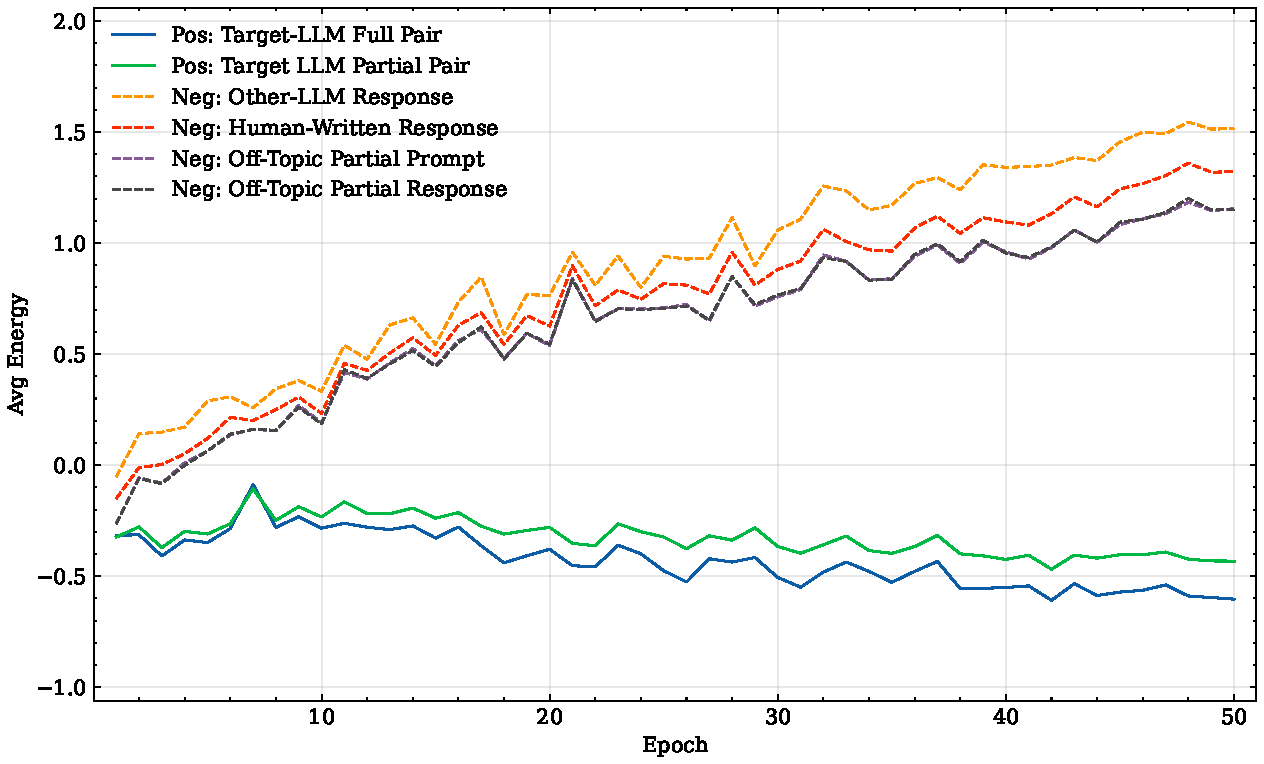
\includegraphics[width=0.48\textwidth]{figures/plot_ebm2s4cwiki_hyb_pretraining_energy.pdf}
    }
    \hfill
    \subfigure[توزیع انرژی در $\mathcal{E}_{\text{\lr{hybrid}}}^{\text{\lr{210M}}}$]{\label{fig:chap5_capacity_energy_210m}
        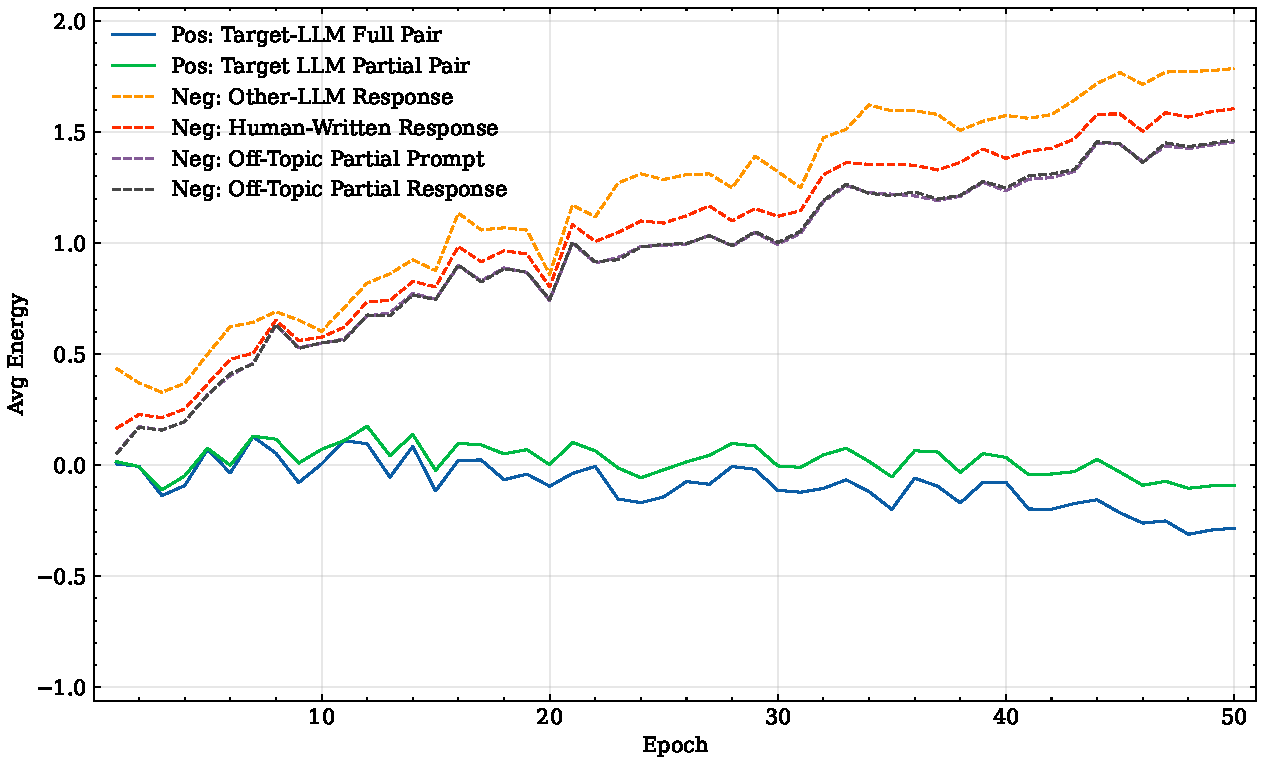
\includegraphics[width=0.48\textwidth]{figures/plot_ebm2s10cwiki_hyb_pretraining_energy.pdf}
    }
    \vspace{-0.25cm}
    \caption{مقایسه‌ی توزیع انرژی اعتبارسنجی در مدل‌های ۱۶۷ و ۲۱۰ میلیون پارامتری}\label{fig:chap5_capacity_energy}
\end{figure}
\vspace{-0.75cm}
\begin{figure}[!ht]
    \centering
    \subfigure[روند خطا در $\mathcal{E}_{\text{\lr{hybrid}}}^{\text{\lr{167M}}}$]{\label{fig:chap5_capacity_loss_167m}
        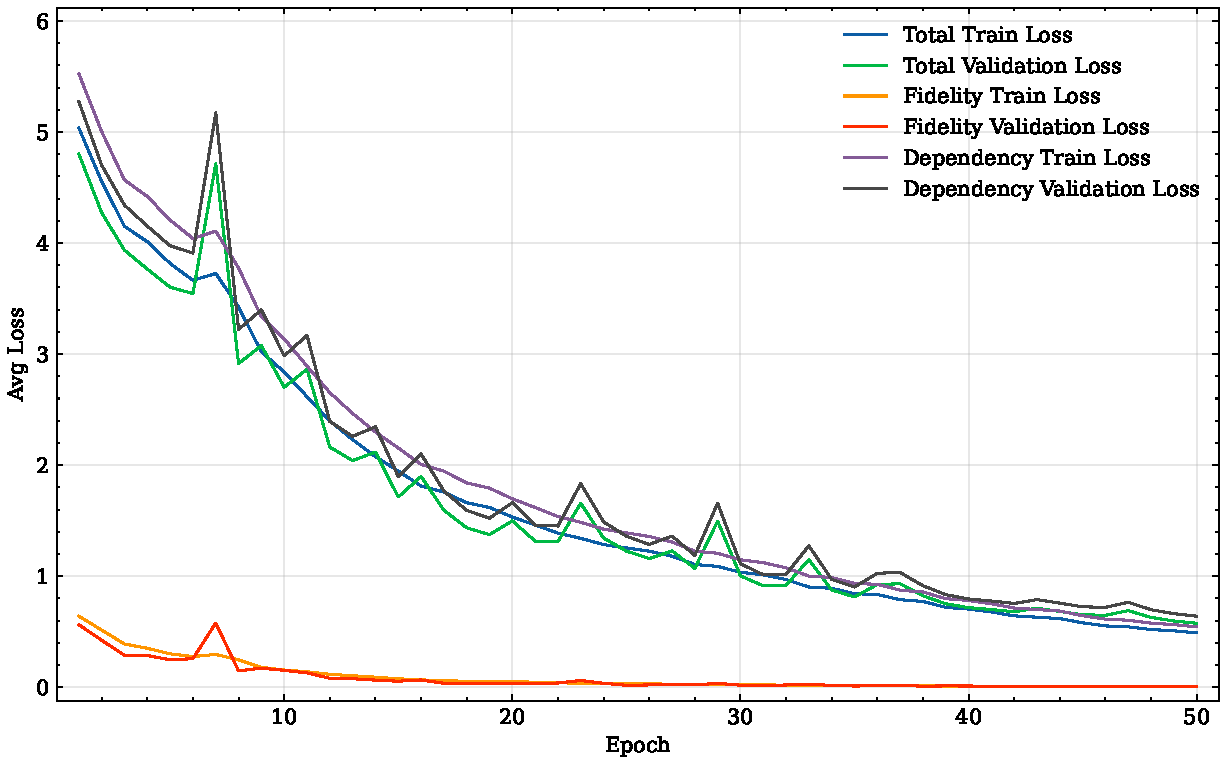
\includegraphics[width=0.48\textwidth]{figures/plot_ebm2s4cwiki_hyb_pretraining_loss.pdf}
    }
    \hfill
    \subfigure[روند خطا در $\mathcal{E}_{\text{\lr{hybrid}}}^{\text{\lr{210M}}}$]{\label{fig:chap5_capacity_loss_210m}
        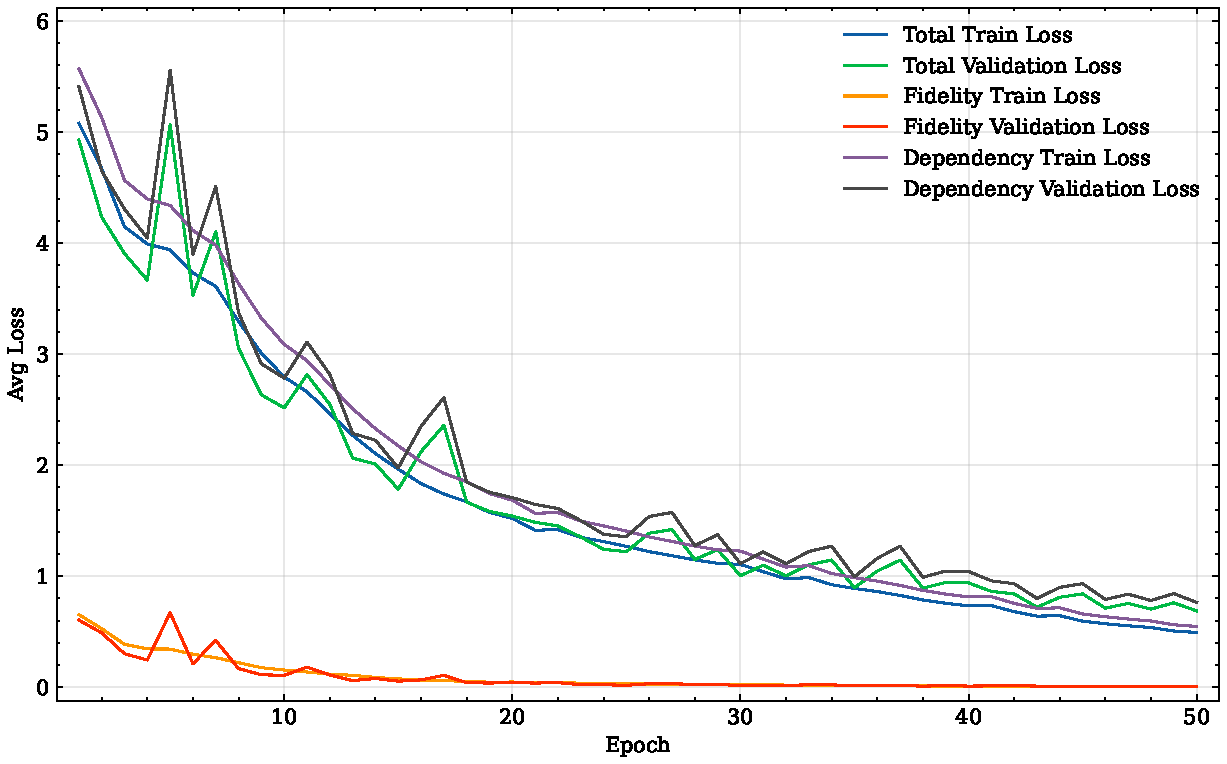
\includegraphics[width=0.48\textwidth]{figures/plot_ebm2s10cwiki_hyb_pretraining_loss.pdf}
    }
    \vspace{-0.25cm}
    \caption{مقایسه‌ی خطای آموزش و اعتبارسنجی در مدل‌های ۱۶۷ و ۲۱۰ میلیون پارامتری.}\label{fig:chap5_capacity_loss}
\end{figure}

نمودارهای توزیع انرژی (شکل~\ref{fig:chap5_capacity_energy}) نشان می‌دهد که در هر دو مدل، انرژی نمونه‌های مثبت به سمت مقادیر منفی سوق یافته و انرژی نمونه‌های منفی روندی افزایشی داشته است. تفاوت شکاف انرژی میان دو مدل ۱۶۷ و ۲۱۰ میلیون پارامتری نسبتاً محدود است که نشان می‌دهد برای پیچیدگی موجود در داده‌های به‌کار رفته، ظرفیت مدل ۱۶۷ میلیونی نیز کفایت بازنمایی لازم را فراهم می‌آورد. روند خطای اعتبارسنجی (شکل~\ref{fig:chap5_capacity_loss}) نیز هم‌گرایی پایدار هر دو مدل را پیش از اتمام ایپاک‌ها تأیید می‌کند.

\paragraph{پویایی توابع زیان و استراتژی‌های یادگیری.}
برای سنجش اثر مستقیم تابع زیان در ظرفیت ثابت، سه مدل ۱۸۱ میلیون پارامتری با توابع زیان وفاداری مطلق ($\mathcal{E}_{\text{\lr{fidelity}}}^{\text{\lr{181M}}}$)، وابستگی محلی مطلق ($\mathcal{E}_{\text{\lr{dependency}}}^{\text{\lr{181M}}}$) و ترکیبی ($\mathcal{E}_{\text{\lr{hybrid}}}^{\text{\lr{181M}}}$) بر روی مجموعه‌داده‌ی \lr{HC3} آموزش داده شدند.

توزیع انرژی و روند خطای این سه مدل در شکل‌های~\ref{fig:chap5_loss_energy} و~\ref{fig:chap5_loss_convergence} مقایسه شده است.

\begin{figure}[!ht]
    \centering
    \subfigure[انرژی در $\mathcal{E}_{\text{\lr{fidelity}}}^{\text{\lr{181M}}}$]{\label{fig:chap5_loss_energy_fid}
        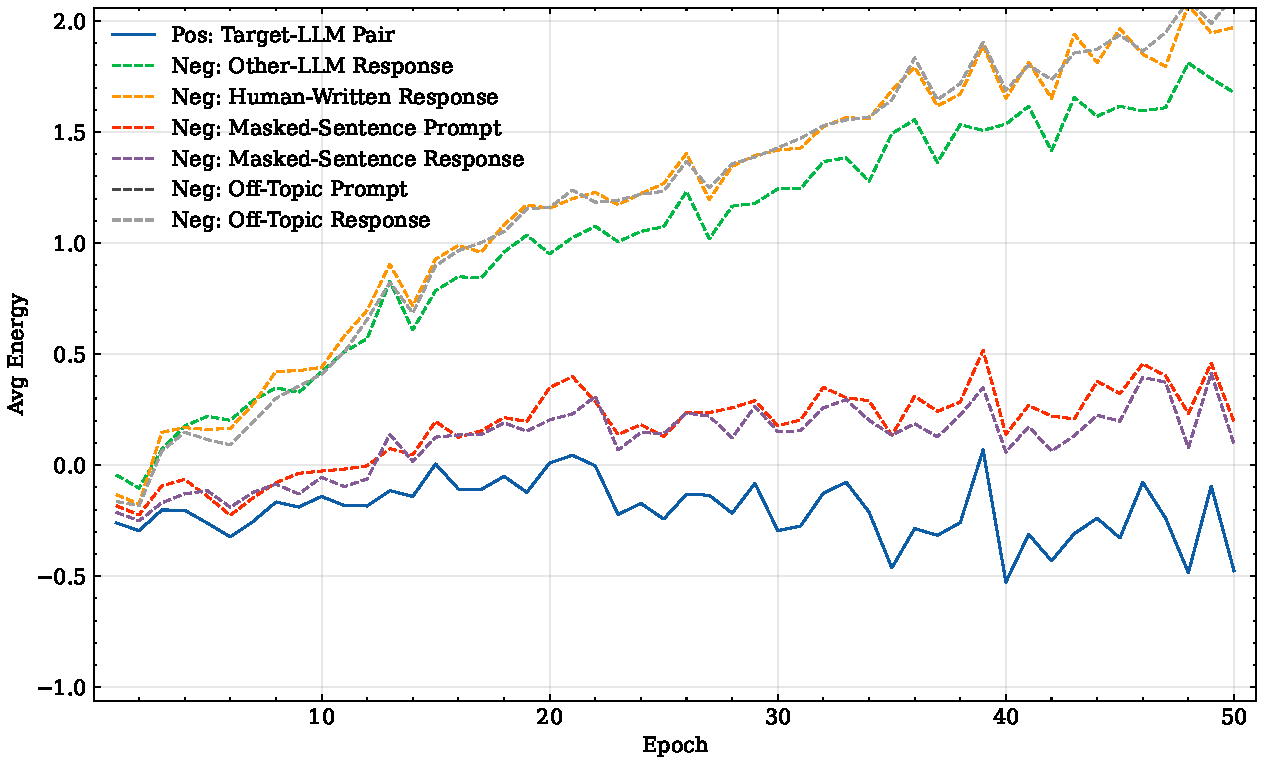
\includegraphics[width=0.31\textwidth]{figures/plot_ebm2s6chc3_fid_pretraining_energy.pdf}
    }%
    \hfill
    \subfigure[انرژی در $\mathcal{E}_{\text{\lr{dependency}}}^{\text{\lr{181M}}}$]{\label{fig:chap5_loss_energy_dep}
        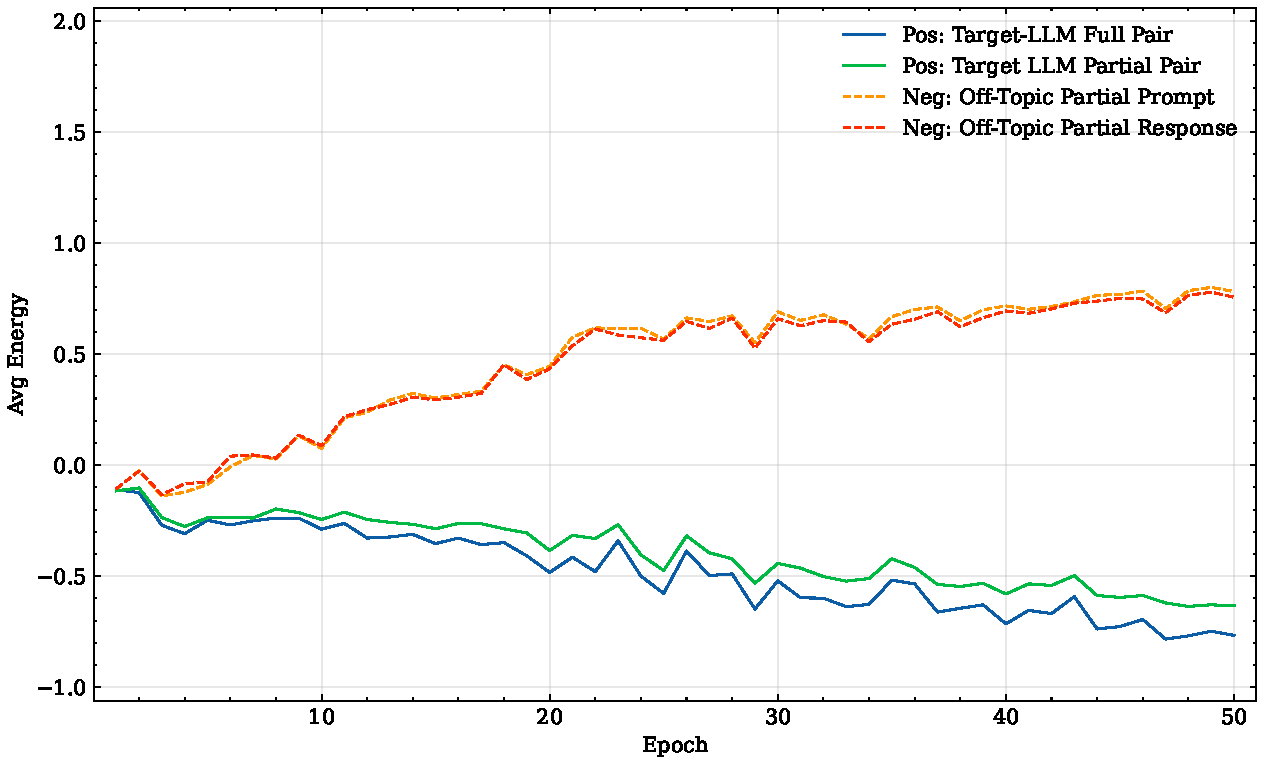
\includegraphics[width=0.31\textwidth]{figures/plot_ebm2s6chc3_dep_pretraining_energy.pdf}
    }%
    \hfill
    \subfigure[انرژی در $\mathcal{E}_{\text{\lr{hybrid}}}^{\text{\lr{181M}}}$]{\label{fig:chap5_loss_energy_hyb}
        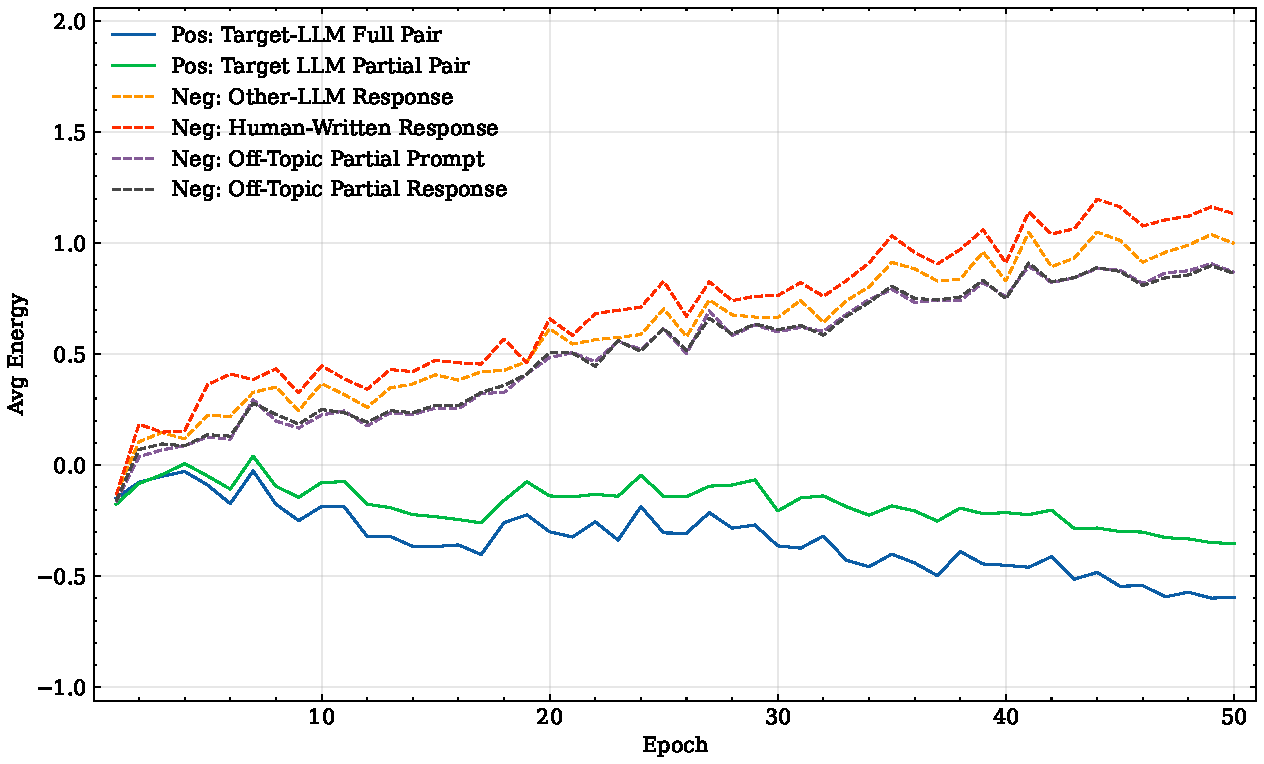
\includegraphics[width=0.31\textwidth]{figures/plot_ebm2s6chc3_hyb_pretraining_energy.pdf}
    }
    \vspace{-0.25cm}
    \caption{مقایسه‌ی توزیع انرژی اعتبارسنجی تحت سه استراتژی یادگیری متفاوت}\label{fig:chap5_loss_energy}
\end{figure}

\begin{figure}[!ht]
    \centering
    \subfigure[خطا در $\mathcal{E}_{\text{\lr{fidelity}}}^{\text{\lr{181M}}}$]{\label{fig:chap5_loss_fid}
        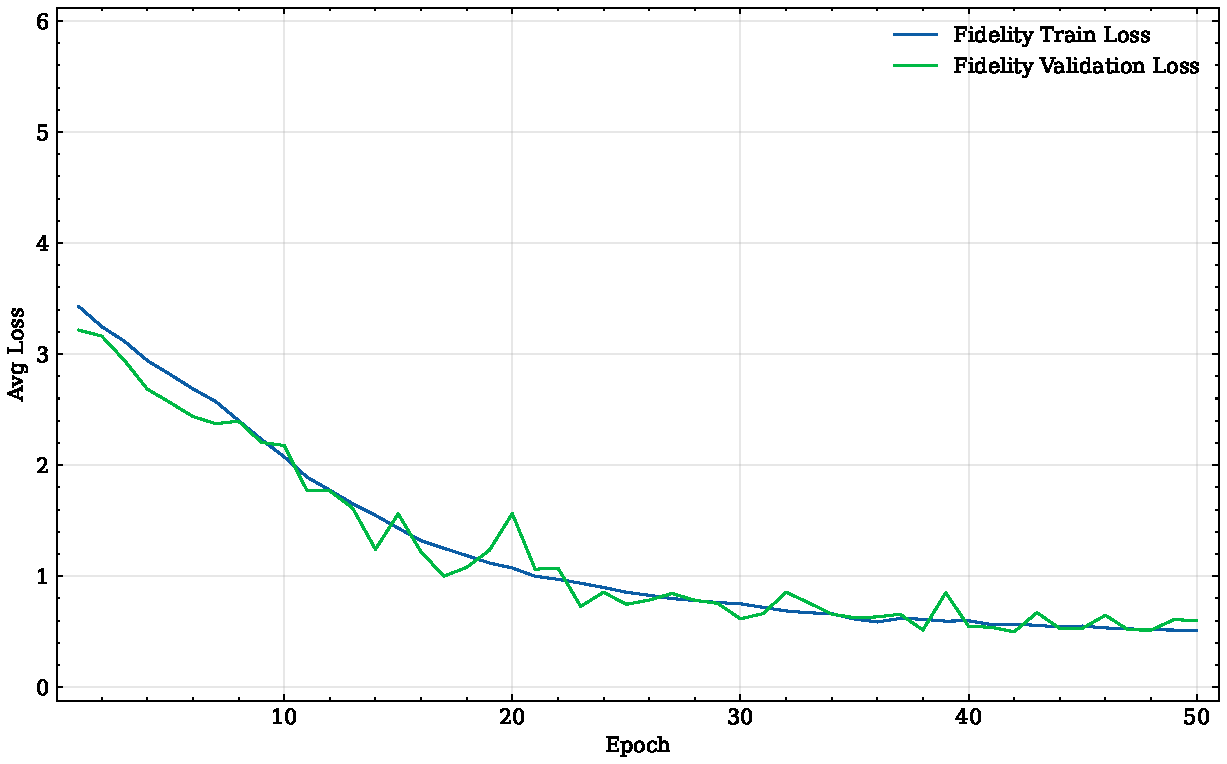
\includegraphics[width=0.31\textwidth]{figures/plot_ebm2s6chc3_fid_pretraining_loss.pdf}
    }%
    \hfill
    \subfigure[خطا در $\mathcal{E}_{\text{\lr{dependency}}}^{\text{\lr{181M}}}$]{\label{fig:chap5_loss_dep}
        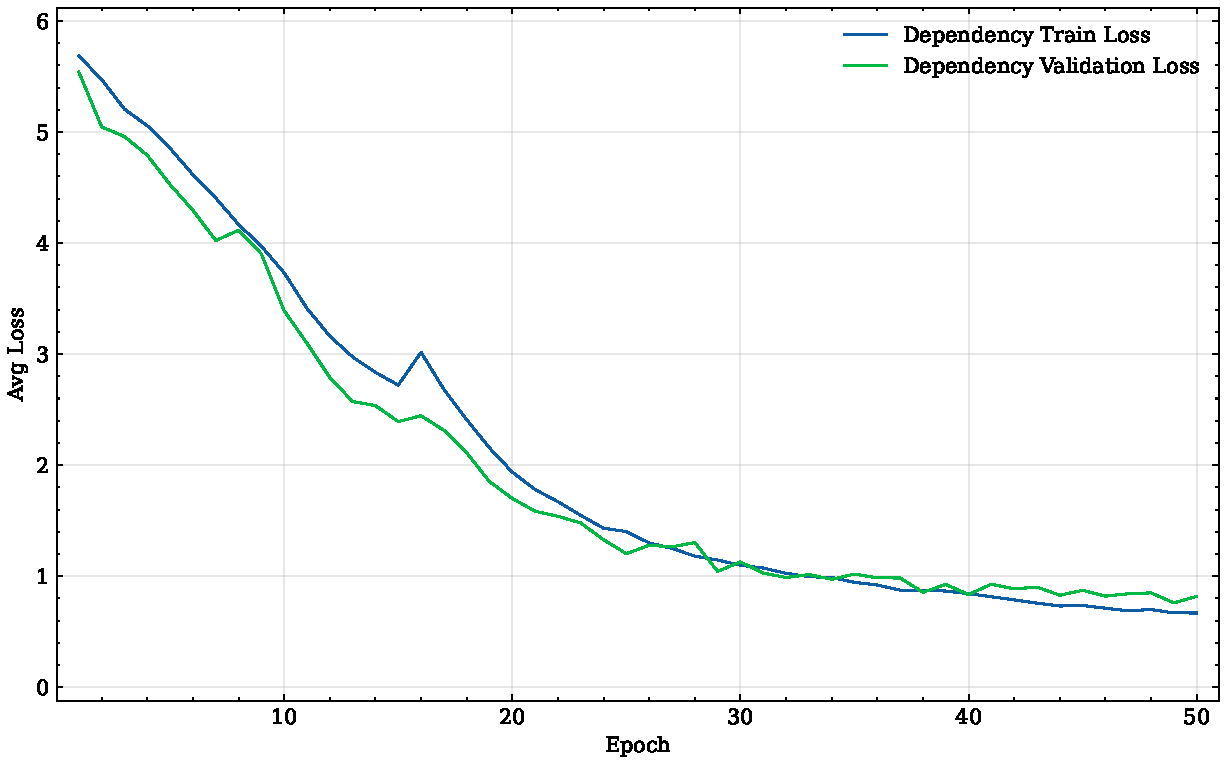
\includegraphics[width=0.31\textwidth]{figures/plot_ebm2s6chc3_dep_pretraining_loss.pdf}
    }%
    \hfill
    \subfigure[خطا در $\mathcal{E}_{\text{\lr{hybrid}}}^{\text{\lr{181M}}}$]{\label{fig:chap5_loss_hyb}
        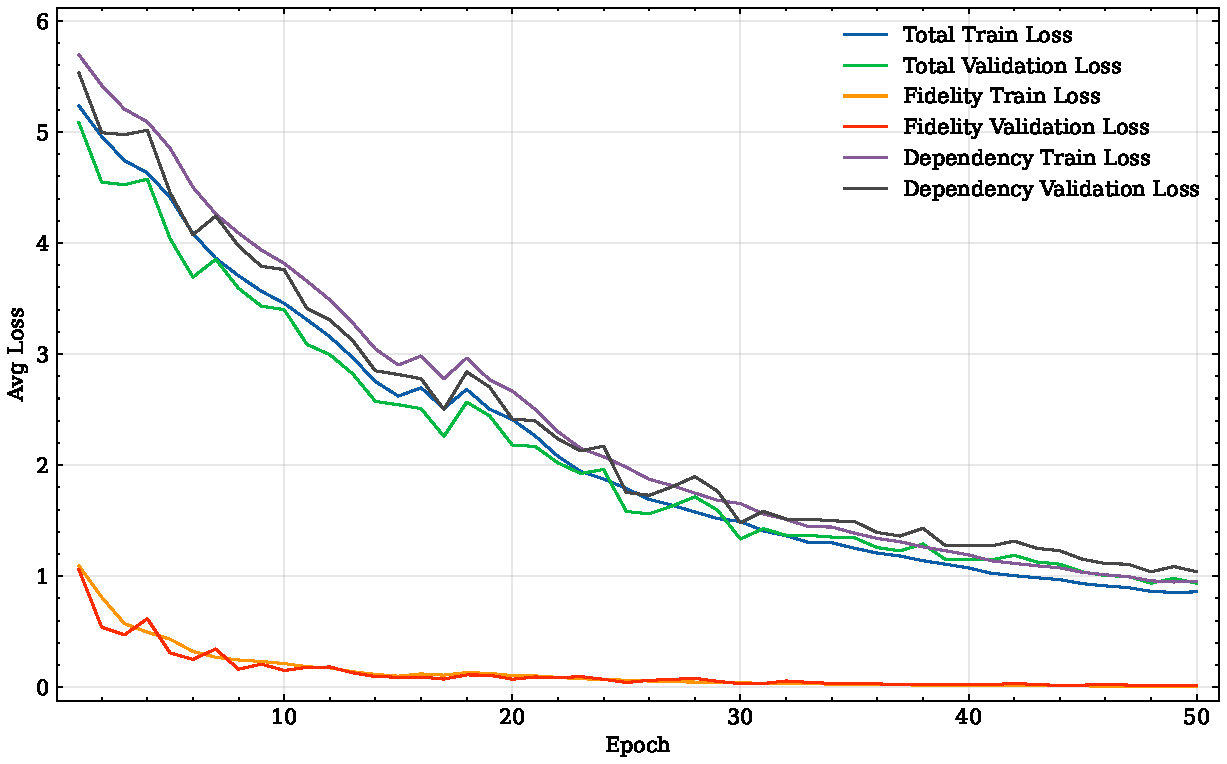
\includegraphics[width=0.31\textwidth]{figures/plot_ebm2s6chc3_hyb_pretraining_loss.pdf}
    }
    \vspace{-0.25cm}
    \caption{مقایسه‌ی خطای آموزش و اعتبارسنجی در سه پیکربندی تابع زیان.}\label{fig:chap5_loss_convergence}
\end{figure}

در شکل~\ref{fig:chap5_loss_energy_fid}، مدل $\mathcal{E}_{\text{\lr{fidelity}}}^{\text{\lr{181M}}}$ شکاف عریضی میان نمونه‌های مثبت و منفی ایجاد کرده است؛ اما همان‌گونه که در تحلیل بخش~\ref{sec:5-2-2} نشان داده شد، بخشی از این تفکیک ناشی از اتکا به آرتیفکت‌های قالبی است. در شکل~\ref{fig:chap5_loss_energy_dep}، مدل $\mathcal{E}_{\text{\lr{dependency}}}^{\text{\lr{181M}}}$ نوسانات کمتری دارد اما شکاف بسته‌تری ایجاد می‌کند. سرانجام، مدل ترکیبی پیشنهادی $\mathcal{E}_{\text{\lr{hybrid}}}^{\text{\lr{181M}}}$ (شکل~\ref{fig:chap5_loss_energy_hyb})، روندی باثبات‌تر ارائه کرده و تعادل مطلوبی میان تفکیک موضعی و پایداری سراسری خمینه‌ی انرژی نشان می‌دهد.


\subsection{تحلیل عملکرد پایین‌دست انرژی بر یادگیری مفسر}\label{sec:5-2-4}

در چارچوب \lr{ESCI}، شبکه‌ی انرژی نقش ارزیاب و منتقد را ایفا می‌کند تا گرادیان‌های لازم را برای آموزش شبکه‌ی مفسر ($\mathcal{IN}$) فراهم آورد. بنابراین، بررسی نحوه‌ی هدایت مفسر توسط مدل‌های انرژی، معیاری کلیدی برای اعتبارسنجی منتقد است.

ارزیابی‌ها نشان داد که مفسر هدایت‌شده توسط مدل وفاداری مطلق ($\mathcal{E}_{\text{\lr{fidelity}}}^{\text{\lr{181M}}}$)، به‌دلیل عدم‌حساسیت منتقد به وابستگی‌های موضعی، ماسک‌هایی مسطح و با خلوتی ناکافی تولید می‌کند. مقایسه‌ی رفتار آموزشی مفسر تحت نظارت دو منتقد دیگر یعنی مدل وابستگی مطلق ($\mathcal{IN}_{\text{\lr{dependency}}}^{\text{\lr{180M}}}$ هدایت‌شده توسط $\mathcal{E}_{\text{\lr{dependency}}}^{\text{\lr{181M}}}$) و مدل ترکیبی ($\mathcal{IN}_{\text{\lr{hybrid}}}^{\text{\lr{180M}}}$ هدایت‌شده توسط $\mathcal{E}_{\text{\lr{hybrid}}}^{\text{\lr{181M}}}$) در شکل~\ref{fig:chap5_interpreter_loss} ترسیم شده است.

\vspace{0.4cm}
\begin{figure}[!ht]
    \centering
    \subfigure[روند خطای مفسر $\mathcal{IN}_{\text{\lr{dependency}}}^{\text{\lr{180M}}}$]{\label{fig:chap5_interpreter_dep_loss}
        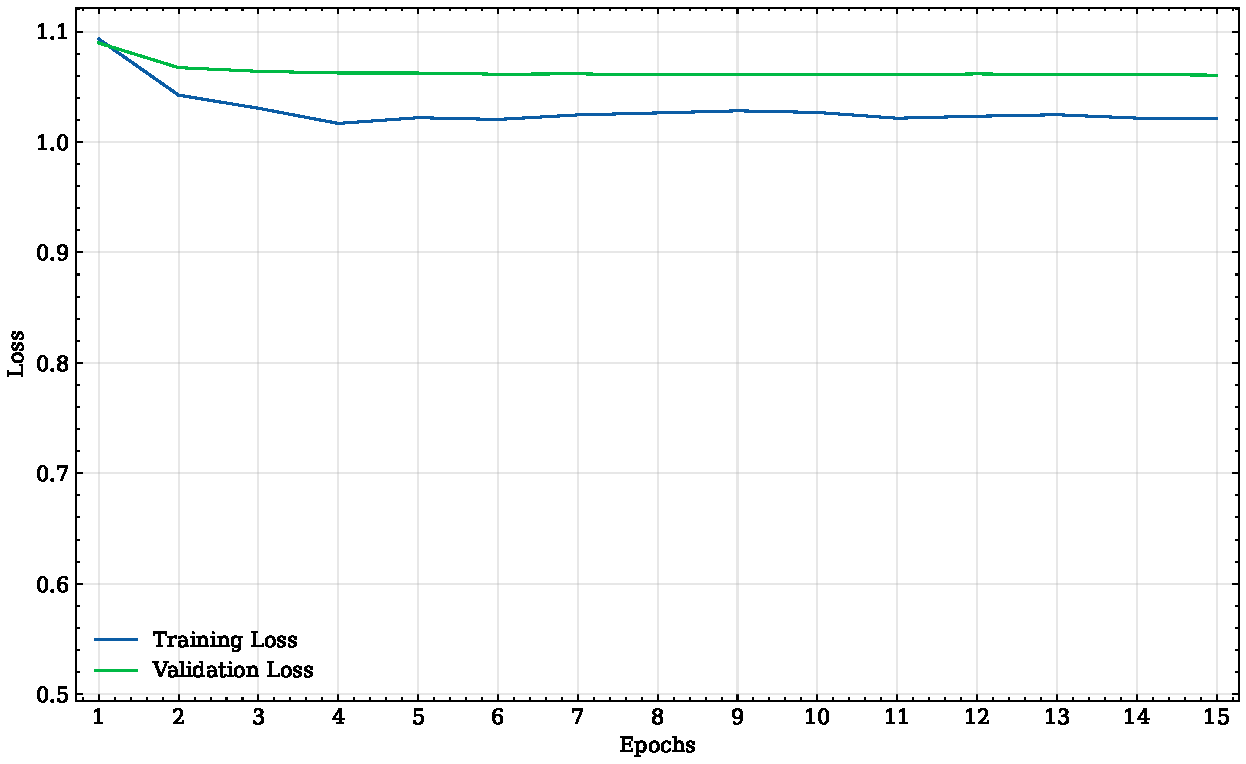
\includegraphics[width=0.48\textwidth]{figures/plot_interpreter1_loss.pdf}
    }
    \hfill
    \subfigure[روند خطای مفسر $\mathcal{IN}_{\text{\lr{hybrid}}}^{\text{\lr{180M}}}$]{\label{fig:chap5_interpreter_hyb_loss}
        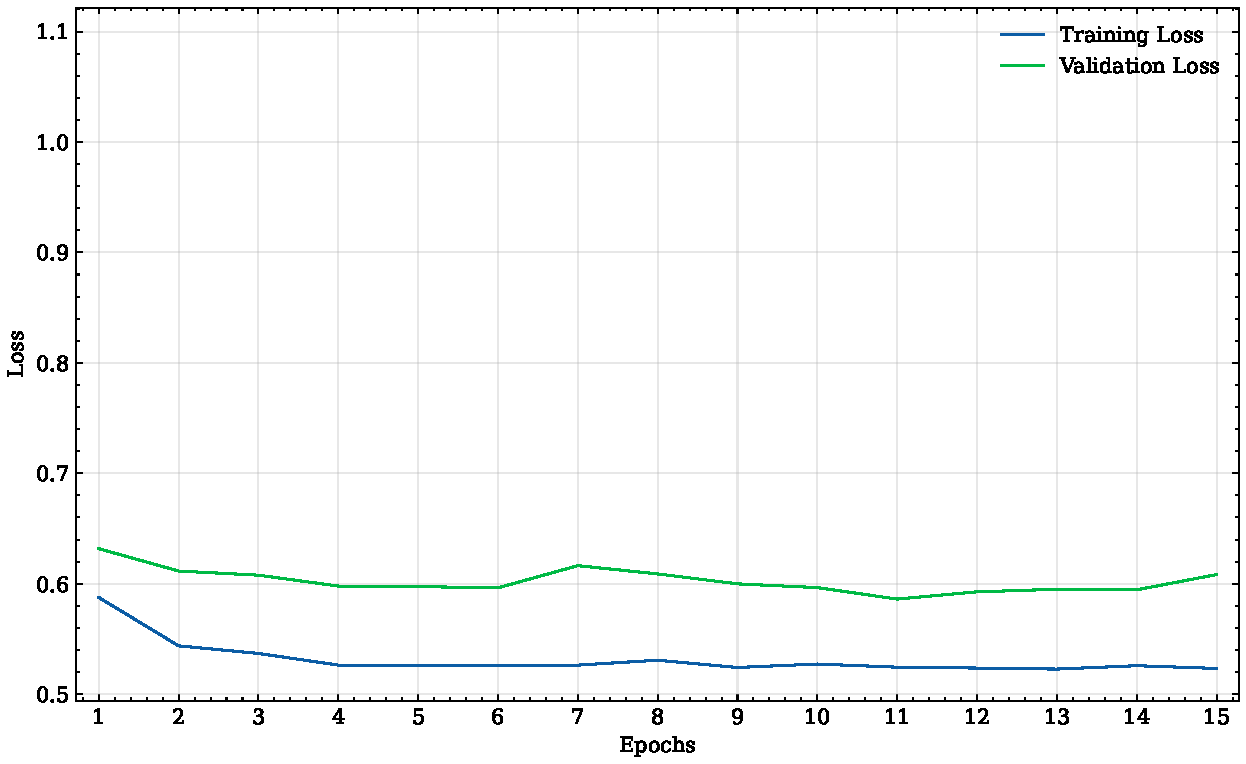
\includegraphics[width=0.48\textwidth]{figures/plot_interpreter2_loss.pdf}
    }
    \vspace{-0.25cm}
    \caption{مقایسه‌ی یادگیری شبکه‌ی مفسر تحت هدایت دو مدل انرژی متفاوت}\label{fig:chap5_interpreter_loss}
\end{figure}
\vspace{0.25cm}

همان‌طور که در شکل~\ref{fig:chap5_interpreter_dep_loss} مشاهده می‌شود، مفسر تحت هدایت $\mathcal{E}_{\text{\lr{dependency}}}$ روند هم‌گرایی کندی داشته و خطای اعتبارسنجی در محدوده‌ی بالای $1.06$ متوقف می‌گردد. در غیاب منظم‌سازی سراسری، خمینه‌ی انرژی در قبال ماسک‌های نرم مفسر، حساسیت شدیدی نشان داده و گرادیان‌هایی با نوسان و ناپایداری بالا تولید می‌کند که بهینه‌سازی مفسر را با دشواری روبه‌رو می‌سازد.

در مقابل، در نمودار ب (شکل~\ref{fig:chap5_interpreter_hyb_loss})، مفسر تحت هدایت مدل ترکیبی $\mathcal{IN}_{\text{\lr{hybrid}}}^{\text{\lr{180M}}}$، کاهش منظم خطا تا محدوده‌ی $0.59$ را تجربه می‌کند. مؤلفه‌ی وفاداری سراسری در تابع زیان منتقد، فضای انرژی را هموارتر ساخته و گرادیان‌های باثبات‌تری برای هدایت مفسر فراهم می‌آورد. این تحلیل تأیید می‌کند که مدل انرژی بهینه باید هم‌زمان از حاشیه‌ی تفکیک موضعی و منظم‌سازی سراسری برخوردار باشد تا یادگیری مفسر به‌صورت پایدار محقق گردد.


\section{ارزیابی مفسر در محیط‌های با دسترسی متفاوت}\label{sec:5-3}

پس از بررسی ویژگی‌های شبکه‌ی جانشین انرژی، این بخش به ارزیابی عملکرد سیستم یکپارچه، یعنی شبکه‌ی مفسر (\lr{ESCI}) می‌پردازد. هدف مفسر، استخراج زیرمجموعه‌ای خلوت از جملات پرامپت است که به‌عنوان پیش‌نیازهای گزاره‌ای در تولید خروجی نقش داشته‌اند. با توجه به چالش‌های ارزیابی در مدل‌های زبانی بزرگ، این بررسی در سه فاز ساختاردهی شده است: نخست، معقولیت انتساب که هم‌خوانی استخراج‌ها را با داوران زبانی و حقایق ساختاریافته می‌سنجد؛ دوم، وفاداری تجربی (شامل معیارهای جامعیت و کفایت) که از طریق مداخله در ورودی، میزان تأثیر گزاره‌های منتخب را می‌سنجد؛ و سوم، بررسی کیفی که نمونه‌های موردی را تحلیل می‌نماید.


\subsection{معقولیت انتساب}\label{sec:5-3-1}

پیش از سنجش پرهزینه‌ی تغییرات عملکردی مدل از طریق مداخله، می‌توان ابتدا معقولیت انتساب را ارزیابی کرد. این ارزیابی بررسی می‌کند که آیا جملات انتخاب‌شده توسط مفسر \lr{ESCI}، از نظر زبان‌شناختی و منطق مفهومی، پیش‌آیند معقولی برای خروجی هدف محسوب می‌شوند یا خیر. 

برای سنجش این مؤلفه، ارزیابی در دو ساختار متمایز انجام می‌پذیرد: نخست در محیط تولید متن آزاد در برابر هیئت اوراکل‌های زبانی (مجموعه‌داده‌ی \lr{HC3})، و سپس در محیط استدلال مقید مبتنی بر داده در برابر شبه‌حقیقت پایه‌ی استخراجی (مجموعه‌داده‌ی \lr{WikiBio}). پیش از بررسی نتایج، ابتدا معیارهای محاسباتی فرمول‌بندی می‌شوند.

\paragraph{فرمول‌بندی معیارهای ارزیابی کمّی.}
از آنجا که خروجی روش‌های مختلف از نظر مقیاس متفاوت است، تمامی خروجی‌ها پیش از ارزیابی نرمال‌سازی شده و مقادیر منفی (در صورت وجود در خروجی برخی روش‌های پایه‌ی کلاسیک) به صفر برش می‌خورند تا مجموع امتیازات اهمیت برای جملات هر پرامپت برابر با $1.0$ گردد. 

مطابق با تعاریف ارائه‌شده در فصل~\ref{chap:chapter1_introduction}، فرض کنید پرامپت ورودی شامل $N$ جمله به‌صورت مذکور یعنی $\mathbf{x} = (x_1, \dots, x_N) \in \mathcal{S}^N$ باشد. بردار $\mathbf{s}_{\text{\lr{ref}}} \in \mathbb{R}^N$ نشان‌دهنده‌ی امتیازات اهمیت در مدل مرجع (حقیقت پایه یا اوراکل)، و بردار $\mathbf{s}_{\text{\lr{pred}}} \in \mathbb{R}^N$ نمایانگر امتیازات پیش‌بینی‌شده توسط مفسر برای گزاره‌های پرامپت است. چنانچه مفسری به‌دلیل ناپایداری آموزش، امتیازات کاملاً یکنواختی به تمامی جملات پرامپت اختصاص دهد (واریانس نزدیک به صفر)، معیارهای آن صفر در نظر گرفته می‌شوند. عملکرد از طریق دو معیار زیر سنجیده می‌شود:

\begin{enumerate}
    \item \textbf{دقت برتر نرم (\lr{SoftAcc}):} از آنجا که در زبان طبیعی ممکن است چندین جمله‌ی مکمل برای پشتیبانی از یک گزاره وجود داشته باشند، تطابق صرفاً بر مبنای تک‌انتخاب اول معیاری بسیار سخت‌گیرانه است. لذا معیار دقت برتر نرم را به‌گونه‌ای تعریف می‌کنیم که بررسی کند آیا جمله‌ی برتر انتخاب‌شده توسط مفسر، درون فهرست اولویت‌های برتر مرجع قرار دارد یا خیر.
    
    از نظر ریاضی، در تعریف این معیار ابتدا اندیس جمله‌ی با بالاترین امتیاز در مفسر مشخص می‌شود: $i^* = \operatorname*{argmax}_{i \in {\{1,\dots,N\}}} {(\mathbf{s}_{\text{\lr{pred}}})}_i$. سپس اگر $s_{\text{\lr{top2}}}$ دومین مقدار بزرگ و یکتا در توزیع مرجع $\mathbf{s}_{\text{\lr{ref}}}$ باشد، دقت نرم به‌صورت زیر تعریف می‌گردد:
    \begin{equation}
        \text{\lr{SoftAcc}} = \mathbb{I}\left[ {(\mathbf{s}_{\text{\lr{ref}}})}_{i^*} \ge s_{\text{\lr{top2}}} \right]
    \end{equation}
    این فرمول‌بندی تضمین می‌کند که اگر مرجع امتیاز یکسانی به دو جمله‌ی کلیدی داده باشد، انتخاب هر یک از آن‌ها توسط مفسر صحیح تلقی گردد.

    \item \textbf{بهره‌ی تجمعی تنزیل‌یافته‌ی نرمال‌شده (\lr{nDCG}):} این معیار کیفیت کل فهرست اولویت‌بندی‌شده توسط مفسر را در قیاس با مرجع داوری می‌کند~\cite{jarvelin2002cumulated}.
    اگر $\pi$ جایگشتی از اندیس‌ها باشد که امتیازات مفسر ($\mathbf{s}_{\text{\lr{pred}}}$) را به‌صورت نزولی مرتب می‌کند (به‌گونه‌ای که $\pi(1)$ اندیس مهم‌ترین جمله از دید مفسر باشد)، بهره‌ی تجمعی (\lr{DCG}) با استفاده از امتیازات مرجع به‌عنوان ارزش واقعی، به‌صورت زیر محاسبه می‌شود:
    \begin{equation}
        \text{\lr{DCG}} = \sum_{j=1}^{N} \frac{{(\mathbf{s}_{\text{\lr{ref}}})}_{\pi(j)}}{\log_2(j+1)}
    \end{equation}
    با تقسیم این مقدار بر بهره‌ی ایده‌آل (\lr{IDCG}) که در آن مرتب‌سازی مستقیماً بر اساس مقادیر نزولی خود $\mathbf{s}_{\text{\lr{ref}}}$ انجام می‌شود، نمره‌ی نرمال‌شده‌ی \lr{nDCG} در بازه‌ی $[0, 1]$ به‌دست می‌آید.
\end{enumerate}

\paragraph{تفسیر ماتریس‌های مقایسه‌ای متقاطع.}
نتایج در قالب ماتریس‌های مقایسه‌ای متقاطع مربعی (با ابعاد متناظر با تعداد مدل‌های مورد ارزیابی) گزارش می‌شوند که در آن‌ها \textbf{سطرها نشان‌دهنده‌ی مدل مفسر (پیش‌بینی‌کننده)} و \textbf{ستون‌ها نشان‌دهنده‌ی مدل مرجع (داور)} می‌باشند.

به بیان دیگر، درایه‌ی واقع در سطر $A$ و ستون $B$ نشان می‌دهد که در صورت فرض مدل $B$ به‌عنوان مرجع، خروجی‌های مدل $A$ تا چه اندازه با آن منطبق است. قطر اصلی این ماتریس‌ها عدد $1.000$ را نشان می‌دهد. تفاوت مقدار درایه‌ی $A,B$ با $B,A$ ناشی از تفاوت توزیع خروجی مدل‌ها (برای مثال، پراکندگی در برابر خلوتی، یا نامتقارن بودن تعریف دقت برتر نرم) است.


\subsubsection{عملکرد روی مجموعه‌داده‌ی \lr{HC3}}\label{sec:5-3-1-1}

همان‌طور که پیش‌تر اشاره شد، در متون آزاد به‌دلیل فقدان برچسب‌های ازپیش‌تعیین‌شده، استفاده از مدل‌های زبانی پیشرفته به‌عنوان اوراکل می‌تواند تقریبی از معقولیت شناختی استخراج‌ها فراهم آورد.

\paragraph{تنظیمات آزمایش.}
مجموعه‌داده‌ی \lr{HC3} به مکالمات و پرسش و پاسخ‌های آزاد اختصاص دارد. برای شبیه‌سازی سناریوی مسدود، مدل تجاری \lr{GPT–4o–Mini} به‌عنوان مدل هدف انتخاب شده است و مفسر \lr{ESCI} بر روی پاسخ‌های این مدل ارزیابی می‌شود. ارزیابی معقولیت بر روی زیرمجموعه‌ای شامل ۲۰۰ جفت پرامپت-پاسخ (شامل حدود ۲۰۰۰ وظیفه‌ی انتساب جمله‌ای یکتا) در برابر هیئت اوراکل‌ها (شامل \lr{Gemini–2.5–Flash}، \lr{GPT–4o–Mini}، \lr{Gemma–2–9B–It}، \lr{Llama–3.1–8B–Instruct} و \lr{Mistral–7B–Instruct–v0.2}) انجام گرفته است. از اوراکل‌ها خواسته شد تا توزیع اهمیت گزاره‌ای جملات پرامپت را در قبال جمله‌ی هدف مشخص گزارش کنند.

\vspace{0.25cm}
\begin{table}[ht]
    \centering
    \footnotesize
    \caption{ماتریس‌های درهم‌ریختگی معقولیت انتساب، مجموعه‌داده‌ی \lr{HC3}}\label{tab:chap5_hc3_plausibility}
    \linespread{1}\selectfont
    \setlength{\tabcolsep}{3.5pt}
    \renewcommand{\arraystretch}{1.5}
    \setlength{\aboverulesep}{0pt}
    \setlength{\belowrulesep}{0pt}

    % --- TOP TABLE ---
    \textbf{(الف) معیار \lr{Soft Top-1 Accuracy}} \\[4pt]
    \begin{tabular}{l !{\color{black}\vline} c !{\color{black}\vline} c !{\color{gray!20}\vrule} c !{\color{gray!20}\vrule} c !{\color{gray!20}\vrule} c !{\color{gray!20}\vrule} c} % chktex 26
        \toprule
        \rowcolor{gray!15} \textbf{\lr{Ref $\leftarrow$ | Interpreter $\downarrow$}} &  \textbf{\lr{ESCI}} & \multicolumn{1}{!{\color{gray!15}\vrule}c}{\textbf{\lr{Gemini–2.5}}} & \multicolumn{1}{!{\color{gray!15}\vrule}c}{\textbf{\lr{GPT–4o–Mini}}} & \multicolumn{1}{!{\color{gray!15}\vrule}c}{\textbf{\lr{Gemma–2}}} & \multicolumn{1}{!{\color{gray!15}\vrule}c}{\textbf{\lr{Llama–3.1}}} & \multicolumn{1}{!{\color{gray!15}\vrule}c}{\textbf{\lr{Mistral–7B}}} \\
        \midrule
        \textbf{\lr{ESCI (Ours)}} & $\mathbf{1.000}$ & $0.750$ & $0.640$ & $0.700$ & $0.720$ & $0.740$ \\
        \midrule
        \lr{Gemini–2.5–Flash} & $0.670$ & $\mathbf{1.000}$ & $\mathbf{0.750}$ & $0.650$ & $0.680$ & $0.670$ \\
        \arrayrulecolor{gray!20}\midrule[0.1pt]
        \lr{GPT–4o–Mini} & $0.600$ & $\mathbf{0.850}$ & $\mathbf{1.000}$ & $0.620$ & $0.640$ & $0.650$ \\
        \arrayrulecolor{gray!20}\midrule[0.1pt]
        \lr{Gemma–2–9B–It} & $0.690$ & $0.650$ & $0.490$ & $\mathbf{1.000}$ & $\mathbf{0.830}$ & $0.780$ \\
        \arrayrulecolor{gray!20}\midrule[0.1pt]
        \lr{Llama–3.1–8B–It} & $\mathbf{0.720}$ & $0.680$ & $0.510$ & $\mathbf{0.850}$ & $\mathbf{1.000}$ & $\mathbf{0.800}$ \\
        \arrayrulecolor{gray!20}\midrule[0.1pt]
        \lr{Mistral–7B–It} & $0.700$ & $0.670$ & $0.520$ & $0.790$ & $0.810$ & $\mathbf{1.000}$ \\
        \arrayrulecolor{black}\bottomrule
    \end{tabular}

    \vspace{0.25cm}

    % --- BOTTOM TABLE ---
    \textbf{(ب) معیار \lr{nDCG}} \\[4pt]
    \begin{tabular}{l !{\color{black}\vline} c !{\color{black}\vline} c !{\color{gray!20}\vrule} c !{\color{gray!20}\vrule} c !{\color{gray!20}\vrule} c !{\color{gray!20}\vrule} c} % chktex 26
        \toprule
        \rowcolor{gray!15} \textbf{\lr{Ref $\leftarrow$ | Interpreter $\downarrow$}} & \textbf{\lr{ESCI}} & \multicolumn{1}{!{\color{gray!15}\vrule}c}{\textbf{\lr{Gemini–2.5}}} & \multicolumn{1}{!{\color{gray!15}\vrule}c}{\textbf{\lr{GPT–4o–Mini}}} & \multicolumn{1}{!{\color{gray!15}\vrule}c}{\textbf{\lr{Gemma–2}}} & \multicolumn{1}{!{\color{gray!15}\vrule}c}{\textbf{\lr{Llama–3.1}}} & \multicolumn{1}{!{\color{gray!15}\vrule}c}{\textbf{\lr{Mistral–7B}}} \\
        \midrule
        \textbf{\lr{ESCI (Ours)}} & $\mathbf{1.000}$ & $0.830$ & $0.790$ & $0.810$ & $0.820$ & $0.830$ \\
        \midrule
        \lr{Gemini–2.5–Flash} & $\mathbf{0.850}$ & $\mathbf{1.000}$ & $\mathbf{0.880}$ & $0.760$ & $0.780$ & $0.790$ \\
        \arrayrulecolor{gray!20}\midrule[0.1pt]
        \lr{GPT–4o–Mini} & $0.770$ & $\mathbf{0.890}$ & $\mathbf{1.000}$ & $0.770$ & $0.790$ & $0.800$ \\
        \arrayrulecolor{gray!20}\midrule[0.1pt]
        \lr{Gemma–2–9B–It} & $0.800$ & $0.750$ & $0.740$ & $\mathbf{1.000}$ & $\mathbf{0.860}$ & $0.830$ \\
        \arrayrulecolor{gray!20}\midrule[0.1pt]
        \lr{Llama–3.1–8B–It} & $0.820$ & $0.770$ & $0.750$ & $\mathbf{0.880}$ & $\mathbf{1.000}$ & $\mathbf{0.850}$ \\
        \arrayrulecolor{gray!20}\midrule[0.1pt]
        \lr{Mistral–7B–It} & $0.810$ & $0.780$ & $0.760$ & $0.820$ & $0.840$ & $\mathbf{1.000}$ \\
        \arrayrulecolor{black}\bottomrule
    \end{tabular}
\end{table}
\vspace{-0.25cm}

\paragraph{تحلیل و مقایسه.}
جدول~\ref{tab:chap5_hc3_plausibility} نتایج ارزیابی معقولیت را برای اوراکل‌ها و مفسر \lr{ESCI} نشان می‌دهد. نتایج حاکی از آن است که مفسر \lr{ESCI} با ساختار سبک خود، به هم‌ترازی بالایی با داوری اوراکل‌های زبانی در انتخاب جملات کلیدی دست یافته است. هنگامی که \lr{ESCI} در نقش مفسر (سطر اول جدول الف) قرار می‌گیرد، تک‌انتخاب برتر آن در $75\%$ مواقع با قضاوت \lr{Gemini-2.5}، در $72\%$ مواقع با \lr{Llama-3.1} و در $74\%$ مواقع با قضاوت \lr{Mistral-7B} هم‌خوانی دارد. این هم‌ترازی در معیار \lr{nDCG} (جدول ب) نیز با کسب امتیازات بالای $0.80$ برای اکثر مدل‌ها تکرار می‌شود و نشان می‌دهد که مدل جانشین توانسته است توزیع اهمیت جملات را به‌شکل مؤثری تقریب بزند.

تفاوت ارقام سطر اول با ستون اول، ناشی از تفاوت رفتار مفسرهاست. اوراکل‌های مولد عموماً مقادیر وزن را به‌صورت گسترده‌تری میان جملات پرامپت پخش می‌کنند؛ در حالی که مفسر \lr{ESCI} به‌دلیل بهره‌گیری از جریمه‌ی پراکندگی $L_1$ در آموزش، ماسک‌هایی خلوت‌تر تولید می‌کند. در نتیجه، انتخاب‌های خلوت \lr{ESCI} غالباً در دامنه‌ی گزینه‌های محتمل اوراکل‌ها قرار می‌گیرد.


\subsubsection{عملکرد روی مجموعه‌داده‌ی \lr{WikiBio}}\label{sec:5-3-1-2}

برای ارزیابی در محیطی مقید با لنگرگاه ساختاریافته، در این بخش عملکرد مفسر بر روی مجموعه‌داده‌ی \lr{WikiBio} سنجیده می‌شود که در آن علاوه بر داوری اوراکل‌ها، خط‌پایه‌ی مکاشفه‌ای تطبیق رشته‌ای (\lr{StringMatching}) نیز به‌عنوان شبه‌حقیقت پایه در دسترس است.

\paragraph{تنظیمات آزمایش.}
پیرو مباحث بخش~\ref{sec:5-1-2-2}، پاسخ‌های این مجموعه‌داده از روی جدول تولید می‌شوند. خط‌پایه‌ی تطبیق رشته‌ای (\lr{StringMatching}) بر مبنای اشتراک واژگانی میان جملات ورودی و خروجی عمل می‌کند. روش‌های مورد ارزیابی دو گروه می‌باشند: روش‌های جعبه‌سیاه (جدول~\ref{tab:chap5_wikibio_plausibility_blackbox}) و روش‌های دارای دسترسی ممتاز (جدول~\ref{tab:chap5_wikibio_plausibility_whitebox}) بر روی مدل هدف \lr{Llama–3.1–8B–It}.

\paragraph{معقولیت انتساب در روش‌های جعبه‌سیاه.}
جدول~\ref{tab:chap5_wikibio_plausibility_blackbox} نتایج را برای روش‌های جعبه‌سیاه نشان می‌دهد. ستون \lr{StringMatching} نقش خط‌پایه‌ی مرجع استخراجی را دارد. نتایج جدول الف نشان می‌دهد که مفسر \lr{ESCI} در $71.2\%$ مواقع، مهم‌ترین جمله‌ی استخراجی خود را با تطابق‌های لغوی موجود در جدول اطلاعات هم‌سو کرده است. نمره‌ی \lr{nDCG} معادل $0.637$ برای \lr{ESCI} در تقابل با این مبنای واژگانی، گویای آن است که خروجی‌های مفسر از معقولیت شناختی مناسبی برخوردارند.

از سوی دیگر، خط‌پایه‌ی \lr{LIME-BlackBox} انطباق $94.4\%$ با \lr{StringMatching} نشان می‌دهد. دلیل این امر، هم‌پوشانی متدولوژیک توابع هدف آن‌هاست؛ \lr{LIME-BlackBox} بر اساس معیار \lr{BERTScore} بهینه‌سازی می‌شود که شباهت واژگانی موضعی را اندازه می‌گیرد و لذا هم‌پوشانی بالایی با تطبیق رشته‌ای پیدا می‌کند. با این حال، همان‌طور که در بخش ارزیابی وفاداری (بخش~\ref{sec:5-3-2}) مشاهده خواهد شد، اشتراک واژگانی لزوماً به معنای شناسایی پیش‌آیندهای مؤثر در تولید متن نیست.

در تقابل مفسر پیشنهادی با هیئت اوراکل‌ها (ستون‌های پایانی جدول~\ref{tab:chap5_wikibio_plausibility_blackbox})، میزان انطباق مفسر با مدل‌هایی نظیر \lr{Gemma-2} و \lr{Llama-3.1} به محدوده‌ی $0.42$ تا $0.44$ می‌رسد و در تقابل با استفاده از \lr{Gemini-2.5-Flash} نیز در سطح $0.59$ است. این موضوع نشان‌دهنده‌ی یک گلوگاه ظرفیتی است؛ در وظیفه‌ی تولید متن از داده‌های جدولی، مدل‌های زبانی عظیم به‌دلیل ابعاد چند میلیارد پارامتری خود، نگاشت‌های دقیق کلید-مقدار را به‌آسانی تفکیک می‌کنند، در حالی که مفسر سبک‌وزن \lr{ESCI} با ۷۱ میلیون پارامتر آموزش‌پذیر، در این تفکیک‌های ریزدانه رفتاری محتاطانه‌تر به نمایش می‌گذارد.

\vspace{0.25cm}
\begin{table}[ht]
    \centering
    \footnotesize
    \caption{ماتریس‌های درهم‌ریختگی معقولیت انتساب، مجموعه‌داده‌ی \lr{WikiBio} (جعبه‌سیاه)}\label{tab:chap5_wikibio_plausibility_blackbox}
    \linespread{1}\selectfont
    \setlength{\tabcolsep}{7.5pt}
    \renewcommand{\arraystretch}{1.5}
    \setlength{\aboverulesep}{0pt}
    \setlength{\belowrulesep}{0pt}

    % --- TOP TABLE ---
    \textbf{(الف) معیار \lr{Soft Top-1 Accuracy}} \\[4pt]
    \begin{tabular}{l !{\color{black}\vline} c !{\color{black}\vline} c !{\color{gray!20}\vrule} c !{\color{gray!20}\vrule} c !{\color{gray!20}\vrule} c !{\color{gray!20}\vrule} c !{\color{gray!20}\vrule} c} % chktex 26
        \toprule
        \rowcolor{gray!15} \textbf{\lr{Ref $\leftarrow$ | Interp. $\downarrow$}} & \textbf{\lr{ESCI}} & \multicolumn{1}{!{\color{gray!15}\vrule}c}{\textbf{\lr{String}}} & \multicolumn{1}{!{\color{gray!15}\vrule}c}{\textbf{\lr{LIME-Blk}}} & \multicolumn{1}{!{\color{gray!15}\vrule}c}{\textbf{\lr{Gemini}}} & \multicolumn{1}{!{\color{gray!15}\vrule}c}{\textbf{\lr{Gemma}}} & \multicolumn{1}{!{\color{gray!15}\vrule}c}{\textbf{\lr{Llama}}} & \multicolumn{1}{!{\color{gray!15}\vrule}c}{\textbf{\lr{Mistral}}} \\
        \midrule
        \textbf{\lr{ESCI (Ours)}} & $\mathbf{1.000}$ & $0.712$ & $0.698$ & $0.591$ & $0.425$ & $0.439$ & $0.496$ \\
        \midrule
        \lr{StringMatching} & $\mathbf{0.991}$ & $\mathbf{1.000}$ & $\mathbf{1.000}$ & $\mathbf{0.880}$ & $\mathbf{0.992}$ & $\mathbf{0.956}$ & $\mathbf{0.981}$ \\
        \arrayrulecolor{gray!20}\midrule[0.1pt]
        \lr{LIME–BlackBox} & $0.395$ & $\mathbf{0.944}$ & $\mathbf{1.000}$ & $0.670$ & $0.524$ & $0.533$ & $0.422$ \\
        \arrayrulecolor{gray!20}\midrule[0.1pt]
        \lr{Gemini–2.5–Flash} & $0.359$ & $0.620$ & $0.610$ & $\mathbf{1.000}$ & $0.450$ & $0.460$ & $0.440$ \\
        \arrayrulecolor{gray!20}\midrule[0.1pt]
        \lr{Gemma–2–9B–It} & $0.362$ & $0.251$ & $0.369$ & $0.470$ & $\mathbf{1.000}$ & $0.791$ & $0.637$ \\
        \arrayrulecolor{gray!20}\midrule[0.1pt]
        \lr{Llama–3.1–8B–It} & $0.357$ & $0.321$ & $0.426$ & $0.480$ & $0.807$ & $\mathbf{1.000}$ & $0.640$ \\
        \arrayrulecolor{gray!20}\midrule[0.1pt]
        \lr{Mistral–7B–It} & $0.485$ & $0.337$ & $0.421$ & $0.450$ & $0.679$ & $0.675$ & $\mathbf{1.000}$ \\
        \arrayrulecolor{black}\bottomrule
    \end{tabular}

    \vspace{0.25cm}

    % --- BOTTOM TABLE ---
    \textbf{(ب) معیار \lr{nDCG}} \\[4pt]
    \begin{tabular}{l !{\color{black}\vline} c !{\color{black}\vline} c !{\color{gray!20}\vrule} c !{\color{gray!20}\vrule} c !{\color{gray!20}\vrule} c !{\color{gray!20}\vrule} c !{\color{gray!20}\vrule} c} % chktex 26
        \toprule
        \rowcolor{gray!15} \textbf{\lr{Ref $\leftarrow$ | Interp. $\downarrow$}} & \textbf{\lr{ESCI}} & \multicolumn{1}{!{\color{gray!15}\vrule}c}{\textbf{\lr{String}}} & \multicolumn{1}{!{\color{gray!15}\vrule}c}{\textbf{\lr{LIME-Blk}}} & \multicolumn{1}{!{\color{gray!15}\vrule}c}{\textbf{\lr{Gemini}}} & \multicolumn{1}{!{\color{gray!15}\vrule}c}{\textbf{\lr{Gemma}}} & \multicolumn{1}{!{\color{gray!15}\vrule}c}{\textbf{\lr{Llama}}} & \multicolumn{1}{!{\color{gray!15}\vrule}c}{\textbf{\lr{Mistral}}} \\
        \midrule
        \textbf{\lr{ESCI (Ours)}} & $\mathbf{1.000}$ & $0.637$ & $0.658$ & $0.621$ & $0.562$ & $0.569$ & $0.615$ \\
        \midrule
        \lr{StringMatching} & $\mathbf{0.741}$ & $\mathbf{1.000}$ & $\mathbf{0.915}$ & $\mathbf{0.860}$ & $\mathbf{0.811}$ & $\mathbf{0.819}$ & $\mathbf{0.765}$ \\
        \arrayrulecolor{gray!20}\midrule[0.1pt]
        \lr{LIME–BlackBox} & $0.646$ & $0.697$ & $\mathbf{1.000}$ & $0.660$ & $0.660$ & $0.676$ & $0.627$ \\
        \arrayrulecolor{gray!20}\midrule[0.1pt]
        \lr{Gemini–2.5–Flash} & $0.577$ & $\mathbf{0.701}$ & $0.687$ & $\mathbf{1.000}$ & $0.550$ & $0.560$ & $0.540$ \\
        \arrayrulecolor{gray!20}\midrule[0.1pt]
        \lr{Gemma–2–9B–It} & $0.493$ & $0.589$ & $0.652$ & $0.560$ & $\mathbf{1.000}$ & $0.805$ & $0.716$ \\
        \arrayrulecolor{gray!20}\midrule[0.1pt]
        \lr{Llama–3.1–8B–It} & $0.478$ & $0.565$ & $0.631$ & $0.570$ & $0.768$ & $\mathbf{1.000}$ & $0.673$ \\
        \arrayrulecolor{gray!20}\midrule[0.1pt]
        \lr{Mistral–7B–It} & $0.579$ & $0.586$ & $0.646$ & $0.550$ & $0.750$ & $0.741$ & $\mathbf{1.000}$ \\
        \arrayrulecolor{black}\bottomrule
    \end{tabular}
\end{table}
\vspace{-0.25cm}

\paragraph{معقولیت انتساب در روش‌های جعبه‌سفید و جعبه‌خاکستری.}
جدول~\ref{tab:chap5_wikibio_plausibility_whitebox} ماتریس‌های متناظر را برای روش‌های دارای دسترسی ممتاز (روش‌های جعبه‌سفید و جعبه‌خاکستری مذکور در بخش~\ref{sec:5-1-3-2}) بر روی مدل هدف \lr{Llama–3.1–8B–It} نشان می‌دهد تا بررسی شود مفسر جعبه‌سیاه \lr{ESCI} تا چه اندازه با روش‌های آگاه از ساختار درونی هم‌سو است.

\begin{table}[ht]
    \centering
    \footnotesize
    \caption{ماتریس‌های درهم‌ریختگی معقولیت انتساب، مجموعه‌داده‌ی \lr{WikiBio} (جعبه‌سفید)}\label{tab:chap5_wikibio_plausibility_whitebox} 
    \linespread{1}\selectfont
    \setlength{\tabcolsep}{6.5pt}
    \renewcommand{\arraystretch}{1.45}
    \setlength{\aboverulesep}{0pt}
    \setlength{\belowrulesep}{0pt}

    % --- TOP TABLE ---
    \textbf{(الف) معیار \lr{Soft Top-1 Accuracy}} \\[4pt]
    \begin{tabular}{l !{\color{black}\vline} c !{\color{black}\vline} c !{\color{gray!20}\vrule} c !{\color{gray!20}\vrule} c !{\color{gray!20}\vrule} c !{\color{gray!20}\vrule} c !{\color{gray!20}\vrule} c !{\color{gray!20}\vrule} c} % chktex 26
        \toprule
        \rowcolor{gray!15} \textbf{\lr{Ref $\leftarrow$ | Interp. $\downarrow$}} & \textbf{\lr{ESCI}} & \multicolumn{1}{!{\color{gray!15}\vrule}c}{\textbf{\lr{String}}} & \multicolumn{1}{!{\color{gray!15}\vrule}c}{\textbf{\lr{Attn.}}} & \multicolumn{1}{!{\color{gray!15}\vrule}c}{\textbf{\lr{Roll.}}} & \multicolumn{1}{!{\color{gray!15}\vrule}c}{\textbf{\lr{G-SHAP}}} & \multicolumn{1}{!{\color{gray!15}\vrule}c}{\textbf{\lr{Inp$\times$G}}} & \multicolumn{1}{!{\color{gray!15}\vrule}c}{\textbf{\lr{S-LOO}}} & \multicolumn{1}{!{\color{gray!15}\vrule}c}{\textbf{\lr{LIME}}} \\
        \midrule
        \textbf{\lr{ESCI (Ours)}} & $\mathbf{1.000}$ & $0.712$ & $0.613$ & $0.712$ & $0.461$ & $0.281$ & $0.581$ & $0.471$ \\
        \midrule
        \lr{StringMatching} & $\mathbf{0.991}$ & $\mathbf{1.000}$ & $\mathbf{1.000}$ & $\mathbf{1.000}$ & $\mathbf{1.000}$ & $\mathbf{1.000}$ & $\mathbf{1.000}$ & $\mathbf{1.000}$ \\
        \arrayrulecolor{gray!20}\midrule[0.1pt]
        \lr{Attention} & $0.665$ & $0.905$ & $\mathbf{1.000}$ & $0.909$ & $0.467$ & $0.286$ & $0.432$ & $0.373$ \\
        \arrayrulecolor{gray!20}\midrule[0.1pt]
        \lr{AttentionRollout} & $0.615$ & $\mathbf{0.996}$ & $0.755$ & $\mathbf{1.000}$ & $0.403$ & $0.310$ & $0.119$ & $0.118$ \\
        \arrayrulecolor{gray!20}\midrule[0.1pt]
        \lr{GradientSHAP} & $0.388$ & $0.346$ & $0.424$ & $0.349$ & $\mathbf{1.000}$ & $0.281$ & $0.488$ & $0.401$ \\
        \arrayrulecolor{gray!20}\midrule[0.1pt]
        \lr{Input$\times$Gradient} & $0.195$ & $0.159$ & $0.229$ & $0.161$ & $0.258$ & $\mathbf{1.000}$ & $0.251$ & $0.196$ \\
        \arrayrulecolor{gray!20}\midrule[0.1pt]
        \lr{SentenceLOO} & $0.263$ & $0.128$ & $0.319$ & $0.129$ & $0.409$ & $0.259$ & $\mathbf{1.000}$ & $0.631$ \\
        \arrayrulecolor{gray!20}\midrule[0.1pt]
        \lr{LIME–GrayBox} & $0.364$ & $0.168$ & $0.355$ & $0.167$ & $0.371$ & $0.205$ & $0.761$ & $\mathbf{1.000}$ \\
        \arrayrulecolor{black}\bottomrule
    \end{tabular}

    \vspace{0.25cm}

    % --- BOTTOM TABLE ---
    \textbf{(ب) معیار \lr{nDCG}} \\[4pt]
    \begin{tabular}{l !{\color{black}\vline} c !{\color{black}\vline} c !{\color{gray!20}\vrule} c !{\color{gray!20}\vrule} c !{\color{gray!20}\vrule} c !{\color{gray!20}\vrule} c !{\color{gray!20}\vrule} c !{\color{gray!20}\vrule} c} % chktex 26
        \toprule
        \rowcolor{gray!15} \textbf{\lr{Ref $\leftarrow$ | Interp. $\downarrow$}} & \textbf{\lr{ESCI}} & \multicolumn{1}{!{\color{gray!15}\vrule}c}{\textbf{\lr{String}}} & \multicolumn{1}{!{\color{gray!15}\vrule}c}{\textbf{\lr{Attn.}}} & \multicolumn{1}{!{\color{gray!15}\vrule}c}{\textbf{\lr{Roll.}}} & \multicolumn{1}{!{\color{gray!15}\vrule}c}{\textbf{\lr{G-SHAP}}} & \multicolumn{1}{!{\color{gray!15}\vrule}c}{\textbf{\lr{Inp$\times$G}}} & \multicolumn{1}{!{\color{gray!15}\vrule}c}{\textbf{\lr{S-LOO}}} & \multicolumn{1}{!{\color{gray!15}\vrule}c}{\textbf{\lr{LIME}}} \\
        \midrule
        \textbf{\lr{ESCI (Ours)}} & $\mathbf{1.000}$ & $0.637$ & $0.743$ & $0.726$ & $0.607$ & $0.508$ & $0.625$ & $0.624$ \\
        \midrule
        \lr{StringMatching} & $0.741$ & $\mathbf{1.000}$ & $\mathbf{0.901}$ & $0.826$ & $0.787$ & $0.713$ & $\mathbf{0.864}$ & $\mathbf{0.930}$ \\
        \arrayrulecolor{gray!20}\midrule[0.1pt]
        \lr{Attention} & $\mathbf{0.760}$ & $\mathbf{0.859}$ & $\mathbf{1.000}$ & $\mathbf{0.929}$ & $\mathbf{0.860}$ & $\mathbf{0.805}$ & $0.863$ & $0.863$ \\
        \arrayrulecolor{gray!20}\midrule[0.1pt]
        \lr{AttentionRollout} & $0.710$ & $0.642$ & $0.882$ & $\mathbf{1.000}$ & $0.631$ & $0.538$ & $0.525$ & $0.544$ \\
        \arrayrulecolor{gray!20}\midrule[0.1pt]
        \lr{GradientSHAP} & $0.581$ & $0.635$ & $0.722$ & $0.697$ & $\mathbf{1.000}$ & $0.627$ & $0.722$ & $0.693$ \\
        \arrayrulecolor{gray!20}\midrule[0.1pt]
        \lr{Input$\times$Gradient} & $0.494$ & $0.584$ & $0.618$ & $0.614$ & $0.630$ & $\mathbf{1.000}$ & $0.626$ & $0.609$ \\
        \arrayrulecolor{gray!20}\midrule[0.1pt]
        \lr{SentenceLOO} & $0.584$ & $0.647$ & $0.679$ & $0.530$ & $0.696$ & $0.568$ & $\mathbf{1.000}$ & $0.825$ \\
        \arrayrulecolor{gray!20}\midrule[0.1pt]
        \lr{LIME–GrayBox} & $0.598$ & $0.724$ & $0.705$ & $0.557$ & $0.691$ & $0.578$ & $0.837$ & $\mathbf{1.000}$ \\
        \arrayrulecolor{black}\bottomrule
    \end{tabular}
\end{table}

نتایج جدول~\ref{tab:chap5_wikibio_plausibility_whitebox} نشان می‌دهد که \lr{ESCI} علی‌رغم عدم‌دسترسی به وزن‌ها، هم‌پوشانی قابل‌توجهی با مکانیسم‌های توجه درونی نشان می‌دهد؛ به‌طوری‌که دقت برتر نرم آن با روش بسط توجه (\lr{AttentionRollout}) برابر با $0.712$ و با توجه خام (\lr{Attention}) معادل $0.613$ است و نمره‌ی \lr{nDCG} آن با این دو روش به ترتیب به $0.726$ و $0.743$ می‌رسد. از آنجا که روش \lr{AttentionRollout} جریان اطلاعات را در لایه‌ها ردیابی می‌کند، تجمیع آن در سطح جمله گزاره‌های با اهمیت را برجسته می‌سازد و هم‌راستایی بالای \lr{ESCI} با آن نشان‌دهنده‌ی تقریب مناسب رفتار توجه است.

در مقابل، روش‌های مبتنی بر گرادیان (\lr{Input$\times$Gradient} و \lr{GradientSHAP}) در این ماتریس انحراف بیشتری با سایر خطوط پایه نشان می‌دهند. برای مثال، دقت نرم روش \lr{Input$\times$Gradient} در تقابل با \lr{ESCI} برابر با $0.195$ است. این امر با مشاهدات پیشین در ادبیات سازگار است؛ گرادیان‌های خام در شبکه‌های عمیق ترنسفورمر به‌دلیل اتصالات باقیمانده و نرمال‌سازی‌های مکرر، دچار اشباع موضعی و نویز فرکانس بالا می‌شوند و تجمیع ساده‌ی آن‌ها در سطح جمله منجر به نوسانات رتبه‌ای می‌گردد. روش \lr{GradientSHAP} از طریق میانگین‌گیری گرادیان بخشی از این نقیصه را جبران می‌کند اما همچنان هم‌پوشانی محدودی ($0.388$) با \lr{ESCI} دارد.

در نهایت، روش‌های مبتنی بر اختلال درونی یعنی \lr{SentenceLOO} و الگوریتم \lr{LIME-GrayBox}، همبستگی بالایی با یکدیگر نشان می‌دهند (دقت نرم $0.761$ و $0.631$، و \lr{nDCG} معادل $0.837$ و $0.825$)، چرا که هر دو اثر اختلال در جملات را بر افت احتمالات خروجی مدل اندازه می‌گیرند. مفسر پیشنهادی \lr{ESCI} نیز هم‌پوشانی مناسبی با \lr{SentenceLOO} (دقت نرم $0.581$ و \lr{nDCG} معادل $0.625$) ثبت کرده است که نشان می‌دهد تقطیر انرژی می‌تواند الگوهای کلی اثرات حذفی را بازنمایی کند.


\subsection{وفاداری تجربی در مدل‌های مولد}\label{sec:5-3-2}

اگرچه نتایج بخش پیشین نشان داد که استخراج‌های مفسر \lr{ESCI} از نظر معنایی با داوری اوراکل‌ها و حقایق ساختاریافته هم‌پوشانی دارند، اما معقولیت انتساب لزوماً به معنای بازتاب دقیق وابستگی‌های رفتاری مدل هدف نیست؛ پدیده‌ای که در ادبیات پژوهش تحت عنوان توهم تفسیرپذیری مورد بحث قرار گرفته است~\cite{friedman2024interpretability}. 

برای بررسی اینکه آیا جملات استخراج‌شده تأثیر عملکردی مستقیمی در فرایند تولید دارند، رفتار مدل از طریق اعمال مداخلات کنترل‌شده در پرامپت ورودی مورد ارزیابی قرار می‌گیرد~\cite{atanasova2023faithfulness}. در این چارچوب، یک مفسر وفادار باید دو شرط را برآورده سازد:

مطابق با تعاریف ارائه‌شده در فصل~\ref{chap:chapter1_introduction} (تعاریف~\ref{def:chap1_proposition_space}،\;~\ref{def:chap1_target_subset} و~\ref{def:chap1_mask_space})، فرض کنید پرامپت اولیه شامل دنباله‌ای از $N$ جمله به‌صورت $\mathbf{x} = (x_1, \dots, x_N) \in \mathcal{S}^N$ باشد و گزاره‌ی هدف خروجی با $y_t \in \mathcal{S}$ (یا زیرمجموعه‌ی هدف $\mathbf{y}_T \subseteq \mathbf{y}$) مشخص شده باشد. بر اساس بردار ماسک دودویی استخراج‌شده ($\mathbf{m} \in \mathcal{M}$)، زیرمجموعه‌ی پیش‌آیندهای منتخب به‌عنوان $\mathbf{x}_S = \mathbf{x} \odot \mathbf{m}$ و زیرمجموعه‌ی متمم (حذف‌شده) به‌عنوان $\mathbf{x} \setminus \mathbf{x}_S = \mathbf{x} \odot (\mathbf{1} - \mathbf{m})$ تعریف می‌شوند. در این صورت، شروط وفاداری با استفاده از یک عملگر ارزیاب وفاداری یکپارچه ($\mathcal{F}$) به شرح زیر فرمول‌بندی می‌شوند:

نخست \textbf{کفایت} ($\mathcal{S}_{\text{\lr{uff}}}$)، بدین‌معنا که حفظ صرفاً جملات استخراج‌شده باید برای بازتولید خروجی هدف تا حد امکان کافی باشد:
\begin{equation}\label{eq:chap5_sufficiency_base}
    \mathcal{S}_{\text{\lr{uff}}} = \mathcal{F}\Big(f_\theta(\mathbf{x}_S), y_t\Big)
\end{equation}

و دوم \textbf{جامعیت} ($\mathcal{C}_{\text{\lr{omp}}}$)، بدین‌معنا که حذف جملات استخراج‌شده از پرامپت، باید منجر به افت توانایی مدل در بازتولید خروجی هدف گردد تا ضرورت حضور آن جملات ارزیابی شود:
\begin{equation}\label{eq:chap5_comprehensiveness_base}
    \mathcal{C}_{\text{\lr{omp}}} = \mathcal{F}\Big(f_\theta(\mathbf{x} \setminus \mathbf{x}_S), y_t\Big)
\end{equation}

در نهایت، \textbf{شکاف وفاداری} ($\Delta\mathcal{F}$) حاصل تفاضل کفایت از جامعیت است:
\begin{equation}\label{eq:chap5_gap_base}
    \Delta\mathcal{F} = \mathcal{S}_{\text{\lr{uff}}} - \mathcal{C}_{\text{\lr{omp}}}
\end{equation}
مقادیر بزرگتر و مثبت $\Delta\mathcal{F}$ نشان‌دهنده‌ی تأثیر متمایز جملات استخراج‌شده در فرایند تولید است.

با توجه به ویژگی‌های زبان طبیعی و امکان بیان یک مفهوم با ساختارهای واژگانی متنوع، تعریف تابع ارزیاب $\mathcal{F}$ با ملاحظات گوناگونی همراه است. برای دستیابی به یک ارزیابی جامع، ما سه سنجه‌ی محاسباتی متمایز را برای $\mathcal{F}$ تعریف و بررسی می‌کنیم: ارزیابی لگاریتم احتمالات نرمال‌شده ($\mathcal{F}_{\text{\lr{logprob}}}$)، ارزیابی شباهت کسینوسی بیشینه‌ی متن تولیدی ($\mathcal{F}_{\text{\lr{cosine}}}$)، و ارزیابی استلزام منطقی صوری ($\mathcal{F}_{\text{\lr{NLI}}}$).


\paragraph{۱. ارزیابی لگاریتم توزیع احتمالات نرمال‌شده ($\mathcal{F}_{\text{\lr{logprob}}}$).}
عینی‌ترین و مرسوم‌ترین روش در ادبیات تفسیرپذیری برای ارزیابی وفاداری، سنجش مستقیم تأثیر مداخله بر روی توزیع احتمالات خروجی مدل است. در این روش، پرامپت مخدوش به‌همراه گزاره‌ی هدف به مدل زبانی داده می‌شود تا بدون نیاز به تولید پاسخی جدید، احتمال تولید همان توکن‌های هدف ارزیابی گردد. تابع لگاریتم احتمالات شرطی برای هر بافتار ورودی $\tilde{\mathbf{x}}$ بر روی توکن‌های گزاره‌ی هدف $y_t = (v_{\sigma_{t-1}+1}, \dots, v_{\sigma_t})$ به‌صورت زیر است:
\begin{equation}
    \mathcal{F}_{\text{\lr{logprob}}}(\tilde{\mathbf{x}}, y_t) = \sum_{j=\sigma_{t-1}+1}^{\sigma_t} \log P_\theta(v_j \mid \tilde{\mathbf{x}}, v_{<j})
\end{equation}
برای امکان مقایسه‌ی مقادیر، این شاخص با روش مقیاس‌دهی با کران نسبی~\cite{carton2020evaluating} نسبت به پرامپت کامل ($\mathcal{F}_{\text{\lr{logprob}}}(\mathbf{x}, y_t)$) و پرامپت خالی ($\mathcal{F}_{\text{\lr{logprob}}}(\emptyset, y_t)$) در بازه‌ی $[0, 1]$ نرمال‌سازی می‌شود:
\begin{align}
    \mathcal{S}_{\text{\lr{logprob}}} &= \max\left(0, \min\left(1, \frac{\mathcal{F}_{\text{\lr{logprob}}}(\mathbf{x}_S, y_t) - \mathcal{F}_{\text{\lr{logprob}}}(\emptyset, y_t)}{\mathcal{F}_{\text{\lr{logprob}}}(\mathbf{x}, y_t) - \mathcal{F}_{\text{\lr{logprob}}}(\emptyset, y_t) + \epsilon}\right)\right) \\
    \mathcal{C}_{\text{\lr{logprob}}} &= \max\left(0, \min\left(1, \frac{\mathcal{F}_{\text{\lr{logprob}}}(\mathbf{x} \setminus \mathbf{x}_S, y_t) - \mathcal{F}_{\text{\lr{logprob}}}(\emptyset, y_t)}{\mathcal{F}_{\text{\lr{logprob}}}(\mathbf{x}, y_t) - \mathcal{F}_{\text{\lr{logprob}}}(\emptyset, y_t) + \epsilon}\right)\right)
\end{align}
و شکاف وفاداری به‌صورت $\Delta\mathcal{F}_{\text{\lr{logprob}}} = \mathcal{S}_{\text{\lr{logprob}}} - \mathcal{C}_{\text{\lr{logprob}}}$ محاسبه می‌شود.

با وجود عینیت ریاضی، تعریف مذکور به سه دلیل با محدودیت روبه‌روست. نخست، این روش نیازمند دسترسی به لوجیت‌های مدل است که در سیستم‌های مسدود فراهم نیست. دوم، همان‌طور که جو و همکاران (۲۰۲۲)~\cite{ju2022logictraps} نشان داده‌اند، تغییر احتمالات در سطح توکن لزوماً به معنای یک تغییر معنادار در استنتاج نیست؛ به بیانی دیگر، افت احتمال تولید دقیقاً همان توکن‌های اولیه‌ی جمله‌ی هدف می‌تواند ناشی از تلاش مدل برای بیان همان مفهوم با بازنویسی و یا شکست کامل مدل به علت ورودی \lr{OOD} باشد. و سوم، بروز استدلال چرخه‌ای در ارزیابی روش‌های مانند \lr{LIME} که خود بر مبنای ایجاد بیشترین شوک توزیعی هستند، معنادار بودن این تعریف وفاداری را زیر سؤال می‌برد.


\paragraph{۲. ارزیابی شباهت کسینوسی بیشینه‌ی متن تولیدی ($\mathcal{F}_{\text{\lr{cosine}}}$).}
در محیط‌های جعبه‌سیاه، دسترسی به احتمالات درونی مدل ناممکن است. در این حالت، مدل زبانی با پرامپت مخدوش تغذیه شده و متن کاملاً جدیدی تولید می‌کند که آن را $\tilde{\mathbf{y}} = (\tilde{y}_1, \dots, \tilde{y}_K) \in \mathcal{S}^K$ می‌نامیم. در این شرایط، سرراست‌ترین روش برای سنجش میزان حفظ بار معنایی در سطح گزاره‌ها بدون درگیر شدن در جزئیات توکن‌ها استفاده از شباهت کسینوسی بر روی تعبیه‌های متراکم جملات (مدل \lr{\texttt{all-mpnet-base-v2}}~\cite{song2020mpnet}) است. با این کار، علاوه بر غلبه بر محدودیت‌های دسترسی، کوری معنایی روش پیشین نیز رفع می‌شود.

لازم به ذکر است که محاسبه‌ی شباهت کسینوسی خطر رقیق‌شدگی اطلاعات در میانگین‌گیری کل پاراگراف را مطرح می‌کند، لذا برای جلوگیری از این چالش، بیشینه‌ی شباهت جملات تولیدشده با گزاره‌ی هدف $y_t$ ملاک قرار می‌گیرد:
\begin{equation}
    \mathcal{F}_{\text{\lr{cosine}}}(\tilde{\mathbf{y}}, y_t) = \max_{k \in \{1, \dots, K\}} \left( \frac{{f_{\text{\lr{sent}}}(y_t)}^\top f_{\text{\lr{sent}}}(\tilde{y}_k)}{{\|f_{\text{\lr{sent}}}(y_t)\|}_2 {\|f_{\text{\lr{sent}}}(\tilde{y}_k)\|}_2} \right)
\end{equation}
با اعمال این تابع بر روی خروجی‌های حاصل از $\mathbf{x}_S$ و $\mathbf{x} \setminus \mathbf{x}_S$، مقادیر کفایت ($\mathcal{S}_{\text{\lr{cosine}}}$) و جامعیت ($\mathcal{C}_{\text{\lr{cosine}}}$) و تفاضل آن‌ها ($\Delta\mathcal{F}_{\text{\lr{cosine}}} = \mathcal{S}_{\text{\lr{cosine}}} - \mathcal{C}_{\text{\lr{cosine}}}$) محاسبه می‌گردد. از آنجا که مدل در زمان تولید آزاد از پارامترهای تصادفی استفاده می‌کند، این نوع آزمایش بر روی ۳ بذر تصادفی مختلف تکرار می‌شود تا واریانس نتایج نیز گزارش شود.

اگرچه این روش می‌تواند ارزیابی را به محیط جعبه‌سیاه و سطح معنا بسط دهد، اما مقایسه‌ی شباهت جملات جدید با جمله‌ی هدف پیشین به‌صورت تکی، با مسئله‌ی گسست اطلاعات مواجه است، چرا که ممکن است مدل زبانی در تولید جدید خود، مفهوم گزاره‌ی هدف را در قالب چند جمله بیان کند.


\paragraph{۳. ارزیابی استلزام منطقی صوری ($\mathcal{F}_{\text{\lr{NLI}}}$).}
برای غلبه بر گسست اطلاعات و حفظ مزیت سنجش متن تولیدشده‌ی جدید از نظر مفهومی و منطقی به‌نسبت گزاره‌ی هدف، از مدل‌های استنتاج زبان طبیعی (\lr{NLI}) نظیر \lr{\texttt{nli-deberta-v3-large}}~\cite{he2023debertav} استفاده می‌کنیم. کل متن پادواقعی تولیدشده ($\tilde{\mathbf{y}}$) به‌عنوان پیش‌فرض و گزاره‌ی هدف ($y_t$) به‌عنوان فرضیه در نظر گرفته می‌شوند. با متمرکز کردن توزیع بر دو کلاس استلزام ($z_{\text{\lr{ent}}}$) و تناقض ($z_{\text{\lr{con}}}$)، تابع ارزیاب استلزام به‌صورت زیر تعریف می‌شود:
\begin{equation}
    \mathcal{F}_{\text{\lr{NLI}}}(\tilde{\mathbf{y}}, y_t) = \frac{\exp(z_{\text{\lr{ent}}})}{\exp(z_{\text{\lr{ent}}}) + \exp(z_{\text{\lr{con}}})}
\end{equation}
و به‌تبع آن، با اعمال این تابع بر روی خروجی‌های حاصل از $\mathbf{x}_S$ و $\mathbf{x} \setminus \mathbf{x}_S$، کفایت ($\mathcal{S}_{\text{\lr{NLI}}}$)، جامعیت ($\mathcal{C}_{\text{\lr{NLI}}}$) و شکاف ($\Delta\mathcal{F}_{\text{\lr{NLI}}} = \mathcal{S}_{\text{\lr{NLI}}} - \mathcal{C}_{\text{\lr{NLI}}}$) تعیین می‌گردند. مجدداً به علت وجود پارامترهای تصادفی، آزمایش بر روی ۳ بذر تصادفی تکرار می‌شود. این سنجه به‌دلیل حساسیت به معنای گزاره‌ای و عدم‌وابستگی به واژگان عین‌به‌عین، معیار مناسبی برای ارزیابی وفاداری تجربی در سطح مفاهیم به‌شمار می‌رود.


\subsubsection{عملکرد روی مجموعه‌داده‌ی \lr{WikiBio}}\label{sec:5-3-2-1}


\paragraph{تنظیمات آزمایش.}
نتایج ارزیابی وفاداری بر روی مجموعه‌داده‌ی \lr{WikiBio} برای دو مدل هدف متن‌باز \lr{Llama–3.1–8B–Instruct} و \lr{Gemma–2–9B–It} در دو گروه روش‌های جعبه‌سیاه (جدول~\ref{tab:chap5_wikibio_faithfulness_blackbox}) و روش‌های دارای دسترسی ممتاز (جدول~\ref{tab:chap5_wikibio_faithfulness_whitebox}) گزارش شده است. ارزیابی‌ها بر روی ۳ بذر تصادفی تکرار شده و میانگین و انحراف معیار آن‌ها درج گردیده است.

\begin{table}[ht]
    \centering
    \caption{نتایج وفاداری تجربی بر روی مجموعه‌داده‌ی \lr{WikiBio} (جعبه‌سیاه)}\label{tab:chap5_wikibio_faithfulness_blackbox}
    \scriptsize 
    \linespread{1}\selectfont
    \setlength{\tabcolsep}{3.2pt}
    \renewcommand{\arraystretch}{1.5}
    \setlength{\aboverulesep}{0pt}
    \setlength{\belowrulesep}{0pt}

    \begin{tabular}{l !{\color{black}\vline} ccc !{\color{black}\vline} ccc} % chktex 26
        \toprule
        \rowcolor{gray!15} & \multicolumn{3}{c|}{\textbf{مدل هدف: \lr{Llama–3.1–8B–Instruct}}} & \multicolumn{3}{c}{\textbf{مدل هدف: \lr{Gemma–2–9B–It}}} \\
        \rowcolor{gray!15} \textbf{مفسر / خط‌پایه} & \textbf{کفایت} ($\mathcal{S}_{\text{\lr{uff}}}$) $\uparrow$ & \textbf{جامعیت} ($\mathcal{C}_{\text{\lr{omp}}}$) $\downarrow$ & \textbf{شکاف} ($\Delta\mathcal{F}$) $\uparrow$ & \textbf{کفایت} ($\mathcal{S}_{\text{\lr{uff}}}$) $\uparrow$ & \textbf{جامعیت} ($\mathcal{C}_{\text{\lr{omp}}}$) $\downarrow$ & \textbf{شکاف} ($\Delta\mathcal{F}$) $\uparrow$ \\
        \midrule
        \multicolumn{7}{c}{\rule[0cm]{0pt}{0.05cm}\textbf{(الف) استلزام منطقی صوری ($\mathcal{F}_{\text{\lr{NLI}}}$)}\vspace{0.05cm}} \\
        \midrule
        \rowcolor{gray!15} \textbf{\lr{ESCI (Ours)}} & $0.620 \pm 0.002$ & $0.512 \pm 0.003$ & $0.108 \pm 0.004$ & $0.800 \pm 0.003$ & $0.572 \pm 0.003$ & $0.228 \pm 0.004$ \\
        \rowcolor{gray!8} \lr{StringMatching} & $0.602 \pm 0.004$ & $0.542 \pm 0.005$ & $0.060 \pm 0.004$ & $0.782 \pm 0.004$ & $0.602 \pm 0.005$ & $0.180 \pm 0.006$ \\
        \rowcolor{gray!8} \lr{Random (Dir.)} & $0.408 \pm 0.004$ & $0.652 \pm 0.006$ & $-0.244 \pm 0.009$ & $0.531 \pm 0.004$ & $0.814 \pm 0.006$ & $-0.283 \pm 0.009$ \\
        \midrule
        \lr{LIME–BlackBox} & $\mathbf{0.659} \pm 0.013$ & $0.529 \pm 0.002$ & $\mathbf{0.131} \pm 0.011$ & $\mathbf{0.839} \pm 0.013$ & $0.589 \pm 0.002$ & $0.250 \pm 0.013$ \\
        \lr{Gemini–2.5–Flash} & $0.625 \pm 0.002$ & $0.505 \pm 0.003$ & $0.120 \pm 0.004$ & $0.805 \pm 0.003$ & $0.565 \pm 0.003$ & $0.240 \pm 0.004$ \\
        \lr{Gemma–2–9B–It} & $0.506 \pm 0.004$ & $\mathbf{0.422} \pm 0.008$ & $0.083 \pm 0.005$ & $0.714 \pm 0.001$ & $\mathbf{0.425} \pm 0.001$ & $\mathbf{0.289} \pm 0.001$ \\
        \lr{Llama–3.1–8B–It} & $0.523 \pm 0.002$ & $0.457 \pm 0.004$ & $0.066 \pm 0.004$ & $0.701 \pm 0.001$ & $0.557 \pm 0.000$ & $0.143 \pm 0.000$ \\
        \lr{Mistral–7B–It} & $0.542 \pm 0.008$ & $0.492 \pm 0.005$ & $0.050 \pm 0.008$ & $0.723 \pm 0.001$ & $0.555 \pm 0.004$ & $0.168 \pm 0.006$ \\
        \midrule
        \multicolumn{7}{c}{\rule[0cm]{0pt}{0.05cm}\textbf{(ب) شباهت کسینوسی بیشینه‌ی جملات ($\mathcal{F}_{\text{\lr{cosine}}}$)}\vspace{0.05cm}} \\
        \midrule
        \rowcolor{gray!15} \textbf{\lr{ESCI (Ours)}} & $0.486 \pm 0.002$ & $0.463 \pm 0.002$ & $0.023 \pm 0.004$ & $0.586 \pm 0.002$ & $0.563 \pm 0.002$ & $0.023 \pm 0.003$ \\
        \rowcolor{gray!8} \lr{StringMatching} & $0.597 \pm 0.004$ & $\mathbf{0.357} \pm 0.003$ & $0.240 \pm 0.006$ & $0.702 \pm 0.004$ & $\mathbf{0.455} \pm 0.003$ & $0.247 \pm 0.006$ \\
        \rowcolor{gray!8} \lr{Random (Dir.)} & $0.472 \pm 0.001$ & $0.579 \pm 0.001$ & $-0.107 \pm 0.002$ & $0.563 \pm 0.001$ & $0.715 \pm 0.001$ & $-0.152 \pm 0.000$ \\
        \midrule
        \lr{LIME–BlackBox} & $\mathbf{0.685} \pm 0.003$ & $0.385 \pm 0.004$ & $\mathbf{0.301} \pm 0.007$ & $\mathbf{0.788} \pm 0.003$ & $0.490 \pm 0.004$ & $\mathbf{0.298} \pm 0.005$ \\
        \lr{Gemini–2.5–Flash} & $0.491 \pm 0.002$ & $0.458 \pm 0.002$ & $0.033 \pm 0.003$ & $0.592 \pm 0.002$ & $0.555 \pm 0.002$ & $0.037 \pm 0.003$ \\
        \lr{Gemma–2–9B–It} & $0.514 \pm 0.001$ & $0.529 \pm 0.001$ & $-0.015 \pm 0.001$ & $0.573 \pm 0.001$ & $0.638 \pm 0.001$ & $-0.065 \pm 0.001$ \\
        \lr{Llama–3.1–8B–It} & $0.460 \pm 0.001$ & $0.560 \pm 0.002$ & $-0.099 \pm 0.001$ & $0.591 \pm 0.003$ & $0.665 \pm 0.001$ & $-0.074 \pm 0.003$ \\
        \lr{Mistral–7B–It} & $0.503 \pm 0.003$ & $0.513 \pm 0.000$ & $-0.010 \pm 0.003$ & $0.631 \pm 0.001$ & $0.602 \pm 0.002$ & $0.029 \pm 0.001$ \\
        \midrule
        \multicolumn{7}{c}{\rule[0cm]{0pt}{0.05cm}\textbf{(ج) لگاریتم توزیع احتمالات نرمال‌شده ($\mathcal{F}_{\text{\lr{logprob}}}$)}\vspace{0.05cm}} \\
        \midrule
        \rowcolor{gray!15} \textbf{\lr{ESCI (Ours)}} & $0.658 \pm 0.000$ & $0.534 \pm 0.000$ & $0.124 \pm 0.000$ & $0.778 \pm 0.000$ & $0.574 \pm 0.000$ & $0.204 \pm 0.000$ \\
        \rowcolor{gray!8} \lr{StringMatching} & $\mathbf{0.922} \pm 0.000$ & $\mathbf{0.197} \pm 0.000$ & $\mathbf{0.725} \pm 0.000$ & $\mathbf{0.972} \pm 0.000$ & $\mathbf{0.247} \pm 0.000$ & $\mathbf{0.725} \pm 0.000$ \\
        \rowcolor{gray!8} \lr{Random (Dir.)} & $0.420 \pm 0.000$ & $0.600 \pm 0.000$ & $-0.180 \pm 0.000$ & $0.570 \pm 0.000$ & $0.700 \pm 0.000$ & $-0.130 \pm 0.000$ \\
        \midrule
        \lr{LIME–BlackBox} & $0.830 \pm 0.000$ & $0.409 \pm 0.000$ & $0.421 \pm 0.000$ & $0.880 \pm 0.000$ & $0.459 \pm 0.000$ & $0.421 \pm 0.000$ \\
        \lr{Gemini–2.5–Flash} & $0.665 \pm 0.000$ & $0.520 \pm 0.000$ & $0.145 \pm 0.000$ & $0.785 \pm 0.000$ & $0.560 \pm 0.000$ & $0.225 \pm 0.000$ \\
        \lr{Gemma–2–9B–It} & $0.471 \pm 0.000$ & $0.527 \pm 0.000$ & $-0.056 \pm 0.000$ & $0.621 \pm 0.000$ & $0.607 \pm 0.000$ & $0.014 \pm 0.000$ \\
        \lr{Llama–3.1–8B–It} & $0.436 \pm 0.000$ & $0.583 \pm 0.000$ & $-0.147 \pm 0.000$ & $0.586 \pm 0.000$ & $0.663 \pm 0.000$ & $-0.077 \pm 0.000$ \\
        \lr{Mistral–7B–It} & $0.510 \pm 0.000$ & $0.574 \pm 0.000$ & $-0.064 \pm 0.000$ & $0.660 \pm 0.000$ & $0.654 \pm 0.000$ & $0.006 \pm 0.000$ \\
        \bottomrule
    \end{tabular}
\end{table}
\vspace{-0.35cm}

\paragraph{وفاداری در روش‌های جعبه‌سیاه.}
تحلیل کمّی داده‌های جدول~\ref{tab:chap5_wikibio_faithfulness_blackbox} نکات زیر را مشخص می‌سازد:
در آزمون استلزام منطقی ($\mathcal{F}_{\text{\lr{NLI}}}$)، خط‌پایه‌ی تصادفی با ثبت شکاف منفی ($-0.244$ در \lr{Llama} و $-0.283$ در \lr{Gemma})، کران پایین تجربی را نشان می‌دهد. مفسر پیشنهادی \lr{ESCI} به شکاف‌های مثبت $0.108 \pm 0.004$ بر روی \lr{Llama} و $0.228 \pm 0.004$ بر روی \lr{Gemma} دست یافته است که بالاتر از خودتوضیحی مدل‌ها (\lr{Llama-3.1} با $0.066$ و \lr{Gemma-2} با $0.143$) و نزدیک به اوراکل \lr{Gemini-2.5-Flash} ($0.120$ و $0.240$) قرار می‌گیرد.

شایان ذکر است که در تمامی روش‌ها، نمره‌ی جامعیت در محدوده‌ی $0.42$ تا $0.60$ باقی مانده و به صفر نرسیده است. این امر نشان‌دهنده‌ی تکیه‌ی مدل‌های زبانی بر دانش پارامتریک درونی در هنگام حذف جملات ورودی است~\cite{kamahi2024counterfactuals}؛ هنگامی که اطلاعات از پرامپت حذف می‌شود، مدل همچنان گزاره‌های باورپذیری تولید می‌کند که ممکن است تا حدی با فرضیه هم‌پوشانی مفهومی داشته باشد.

از طرفی، در آزمون شباهت کسینوسی ($\mathcal{F}_{\text{\lr{cosine}}}$)، خودتوضیحی مدل‌ها با افت مواجه شده و شکاف‌های منفی ثبت می‌کنند، در حالی که \lr{ESCI} با ثبت شکاف مثبت $0.023$ در هر دو مدل، ثبات خود را حفظ کرده است. این نشان‌گر ضعف مدل‌های کوچک متن‌باز برای تحلیل و تفسیر متن در جهت انتساب است.

اما نکته‌ی قابل‌تأمل، رفتار خطوط پایه‌ی مبتنی بر تقریب موضعی واژگانی (\lr{LIME-BlackBox} و \lr{StringMatching}) است که به‌دلیل بهینه‌سازی مستقیم روی توکن‌ها، حساسیت بیشتری به تک‌کلمات داشته و شکاف‌های بالاتری در دو سنجه‌ی آخر کسب کرده‌اند. با این وجود، \lr{ESCI} در آزمون لگاریتم احتمالات ($\mathcal{F}_{\text{\lr{logprob}}}$) نیز شکاف‌های مثبت $0.124$ و $0.204$ را ثبت نموده است.

\begin{table}[!ht]
    \centering
    \caption{نتایج وفاداری تجربی بر روی مجموعه‌داده‌ی \lr{WikiBio} (جعبه‌سفید)}\label{tab:chap5_wikibio_faithfulness_whitebox}
    \scriptsize
    \linespread{1}\selectfont
    \setlength{\tabcolsep}{3.6pt}
    \renewcommand{\arraystretch}{1.5}
    \setlength{\aboverulesep}{0pt}
    \setlength{\belowrulesep}{0pt}

    \begin{tabular}{l !{\color{black}\vline} ccc !{\color{black}\vline} ccc} % chktex 26
        \toprule
        \rowcolor{gray!15} & \multicolumn{3}{c|}{\textbf{مدل هدف: \lr{Llama–3.1–8B–Instruct}}} & \multicolumn{3}{c}{\textbf{مدل هدف: \lr{Gemma–2–9B–It}}} \\
        \rowcolor{gray!15} \textbf{مفسر / خط‌پایه} & \textbf{کفایت} ($\mathcal{S}_{\text{\lr{uff}}}$) $\uparrow$ & \textbf{جامعیت} ($\mathcal{C}_{\text{\lr{omp}}}$) $\downarrow$ & \textbf{شکاف} ($\Delta\mathcal{F}$) $\uparrow$ & \textbf{کفایت} ($\mathcal{S}_{\text{\lr{uff}}}$) $\uparrow$ & \textbf{جامعیت} ($\mathcal{C}_{\text{\lr{omp}}}$) $\downarrow$ & \textbf{شکاف} ($\Delta\mathcal{F}$) $\uparrow$ \\
        \midrule
        \multicolumn{7}{c}{\rule[0cm]{0pt}{0.05cm}\textbf{(الف) استلزام منطقی صوری ($\mathcal{F}_{\text{\lr{NLI}}}$)}\vspace{0.05cm}} \\
        \midrule
        \rowcolor{gray!15} \textbf{\lr{ESCI (Ours)}} & $0.620 \pm 0.002$ & $0.512 \pm 0.003$ & $0.108 \pm 0.004$ & $0.800 \pm 0.003$ & $0.572 \pm 0.003$ & $0.228 \pm 0.004$ \\
        \rowcolor{gray!8} \lr{StringMatching} & $0.602 \pm 0.004$ & $0.542 \pm 0.005$ & $0.060 \pm 0.004$ & $0.782 \pm 0.004$ & $0.602 \pm 0.005$ & $0.180 \pm 0.006$ \\
        \rowcolor{gray!8} \lr{Random (Dir.)} & $0.408 \pm 0.004$ & $0.652 \pm 0.006$ & $-0.244 \pm 0.009$ & $0.531 \pm 0.004$ & $0.814 \pm 0.006$ & $-0.283 \pm 0.009$ \\
        \midrule
        \lr{Attention} & $0.725 \pm 0.013$ & $0.632 \pm 0.005$ & $0.093 \pm 0.018$ & $\mathbf{0.943} \pm 0.004$ & $0.859 \pm 0.002$ & $0.084 \pm 0.004$ \\
        \lr{AttentionRollout} & $0.725 \pm 0.004$ & $0.632 \pm 0.010$ & $0.093 \pm 0.012$ & $\mathbf{0.943} \pm 0.007$ & $0.859 \pm 0.003$ & $0.084 \pm 0.010$ \\
        \lr{GradientSHAP} & $0.609 \pm 0.014$ & $0.499 \pm 0.005$ & $0.111 \pm 0.019$ & $0.817 \pm 0.003$ & $0.656 \pm 0.004$ & $0.160 \pm 0.003$ \\
        \lr{Input$\times$Gradient} & $0.520 \pm 0.003$ & $0.547 \pm 0.007$ & $-0.027 \pm 0.010$ & $0.665 \pm 0.005$ & $0.636 \pm 0.009$ & $0.029 \pm 0.013$ \\
        \lr{SentenceLOO} & $0.606 \pm 0.007$ & $\mathbf{0.483} \pm 0.002$ & $0.123 \pm 0.009$ & $0.882 \pm 0.009$ & $0.588 \pm 0.006$ & $\mathbf{0.295} \pm 0.003$ \\
        \lr{LIME–GrayBox} & $\mathbf{0.636} \pm 0.010$ & $0.487 \pm 0.003$ & $\mathbf{0.149} \pm 0.007$ & $0.816 \pm 0.010$ & $\mathbf{0.547} \pm 0.003$ & $0.269 \pm 0.010$ \\
        \midrule
        \multicolumn{7}{c}{\rule[0cm]{0pt}{0.05cm}\textbf{(ب) شباهت کسینوسی بیشینه‌ی جملات ($\mathcal{F}_{\text{\lr{cosine}}}$)}\vspace{0.05cm}} \\
        \midrule
        \rowcolor{gray!15} \textbf{\lr{ESCI (Ours)}} & $0.486 \pm 0.002$ & $0.463 \pm 0.002$ & $0.023 \pm 0.004$ & $0.586 \pm 0.002$ & $0.563 \pm 0.002$ & $0.023 \pm 0.003$ \\
        \rowcolor{gray!8} \lr{StringMatching} & $0.597 \pm 0.004$ & $\mathbf{0.357} \pm 0.003$ & $0.240 \pm 0.006$ & $0.702 \pm 0.004$ & $0.455 \pm 0.003$ & $0.247 \pm 0.006$ \\
        \rowcolor{gray!8} \lr{Random (Dir.)} & $0.472 \pm 0.001$ & $0.579 \pm 0.001$ & $-0.107 \pm 0.002$ & $0.563 \pm 0.001$ & $0.715 \pm 0.001$ & $-0.152 \pm 0.000$ \\
        \midrule
        \lr{Attention} & $\mathbf{0.739} \pm 0.003$ & $\mathbf{0.036} \pm 0.005$ & $\mathbf{0.702} \pm 0.004$ & $\mathbf{0.893} \pm 0.000$ & $\mathbf{0.068} \pm 0.002$ & $\mathbf{0.825} \pm 0.002$ \\
        \lr{AttentionRollout} & $\mathbf{0.739} \pm 0.004$ & $\mathbf{0.036} \pm 0.001$ & $\mathbf{0.702} \pm 0.004$ & $\mathbf{0.893} \pm 0.002$ & $\mathbf{0.068} \pm 0.001$ & $\mathbf{0.825} \pm 0.001$ \\
        \lr{GradientSHAP} & $0.590 \pm 0.003$ & $0.422 \pm 0.004$ & $0.168 \pm 0.003$ & $0.778 \pm 0.001$ & $0.449 \pm 0.001$ & $0.329 \pm 0.001$ \\
        \lr{Input$\times$Gradient} & $0.482 \pm 0.004$ & $0.537 \pm 0.001$ & $-0.055 \pm 0.001$ & $0.628 \pm 0.002$ & $0.642 \pm 0.002$ & $-0.014 \pm 0.003$ \\
        \lr{SentenceLOO} & $0.567 \pm 0.003$ & $0.446 \pm 0.003$ & $0.121 \pm 0.006$ & $0.753 \pm 0.003$ & $0.451 \pm 0.001$ & $0.302 \pm 0.001$ \\
        \lr{LIME–GrayBox} & $0.613 \pm 0.005$ & $0.378 \pm 0.003$ & $0.235 \pm 0.002$ & $0.715 \pm 0.005$ & $0.480 \pm 0.004$ & $0.235 \pm 0.004$ \\
        \midrule
        \multicolumn{7}{c}{\rule[0cm]{0pt}{0.05cm}\textbf{(ج) لگاریتم توزیع احتمالات نرمال‌شده ($\mathcal{F}_{\text{\lr{logprob}}}$)}\vspace{0.05cm}} \\
        \midrule
        \rowcolor{gray!15} \textbf{\lr{ESCI (Ours)}} & $0.658 \pm 0.000$ & $0.534 \pm 0.000$ & $0.124 \pm 0.000$ & $0.778 \pm 0.000$ & $0.574 \pm 0.000$ & $0.204 \pm 0.000$ \\
        \rowcolor{gray!8} \lr{StringMatching} & $0.922 \pm 0.000$ & $0.197 \pm 0.000$ & $0.725 \pm 0.000$ & $0.972 \pm 0.000$ & $0.247 \pm 0.000$ & $0.725 \pm 0.000$ \\
        \rowcolor{gray!8} \lr{Random (Dir.)} & $0.420 \pm 0.000$ & $0.600 \pm 0.000$ & $-0.180 \pm 0.000$ & $0.570 \pm 0.000$ & $0.700 \pm 0.000$ & $-0.130 \pm 0.000$ \\
        \midrule
        \lr{Attention} & $\mathbf{1.000} \pm 0.000$ & $\mathbf{0.000} \pm 0.000$ & $\mathbf{1.000} \pm 0.000$ & $\mathbf{1.000} \pm 0.000$ & $\mathbf{0.000} \pm 0.000$ & $\mathbf{1.000} \pm 0.000$ \\
        \lr{AttentionRollout} & $\mathbf{1.000} \pm 0.000$ & $\mathbf{0.000} \pm 0.000$ & $\mathbf{1.000} \pm 0.000$ & $\mathbf{1.000} \pm 0.000$ & $\mathbf{0.000} \pm 0.000$ & $\mathbf{1.000} \pm 0.000$ \\
        \lr{GradientSHAP} & $0.795 \pm 0.000$ & $0.430 \pm 0.000$ & $0.365 \pm 0.000$ & $0.897 \pm 0.000$ & $0.428 \pm 0.000$ & $0.468 \pm 0.000$ \\
        \lr{Input$\times$Gradient} & $0.623 \pm 0.000$ & $0.593 \pm 0.000$ & $0.029 \pm 0.000$ & $0.682 \pm 0.000$ & $0.654 \pm 0.000$ & $0.028 \pm 0.000$ \\
        \lr{SentenceLOO} & $0.869 \pm 0.000$ & $0.342 \pm 0.000$ & $0.527 \pm 0.000$ & $0.970 \pm 0.000$ & $0.385 \pm 0.000$ & $0.584 \pm 0.000$ \\
        \lr{LIME–GrayBox} & $\mathbf{0.957} \pm 0.000$ & $\mathbf{0.143} \pm 0.000$ & $\mathbf{0.814} \pm 0.000$ & $\mathbf{0.987} \pm 0.000$ & $\mathbf{0.173} \pm 0.000$ & $\mathbf{0.814} \pm 0.000$ \\
        \bottomrule
    \end{tabular}
\end{table}

\paragraph{وفاداری در روش‌های جعبه‌سفید و جعبه‌خاکستری.}
داده‌های جدول~\ref{tab:chap5_wikibio_faithfulness_whitebox} نیز نکاتی را روشن می‌سازد.

در طیف لگاریتم احتمالات توکن‌ها (جدول ج)، روش‌های مبتنی بر توجه (\lr{Attention} و \lr{AttentionRollout}) به سقف نظری $1.000$ و خط‌پایه‌ی \lr{LIME-GrayBox} به شکاف $0.814$ دست یافته‌اند. این عملکرد ناشی از دسترسی ممتاز به گراف محاسباتی است؛ این روش‌ها مستقیماً پارامترهایی را منعکس می‌کنند که توزیع احتمالاتی توکن‌ها را شکل می‌دهند. با این وجود، همان‌گونه که در مباحث نظری اشاره شد~\cite{ju2022logictraps}، ارزیابی روش‌هایی که بر پایه‌ی کمینه‌سازی افت احتمالات توکن‌ها عمل می‌کنند با همان سنجه، با چالش استدلال دُوری همراه است و لزوماً به معنای انطباق در سطح گزاره‌ها نیست.

در آزمون استلزام منطقی صوری (جدول الف)، شکاف وفاداری روش‌های \lr{Attention} و \lr{AttentionRollout} به $0.093$ در \lr{Llama} و $0.084$ در \lr{Gemma} تعدیل می‌شود که نشان می‌دهد تانسورهای توجه لزوماً جریان استدلال معنایی در تولید جدید را بازتاب نمی‌دهند. در این سنجه، مفسر پیشنهادی \lr{ESCI} که در محیط جعبه‌سیاه آموزش دیده و دسترسی به وزن‌ها یا گرادیان‌ها ندارد، با ثبت شکاف‌های $0.108$ و $0.228$، عملکردی بالاتر از مکانیسم‌های توجه داخلی نشان داده و به روش‌های اختلالی ممتاز یعنی \lr{SentenceLOO} ($0.123$ و $0.295$) و \lr{LIME-GrayBox} ($0.149$ و $0.269$) نزدیک می‌شود. مزیت این امر زمانی برجسته می‌گردد که توجه شود \lr{SentenceLOO} نیازمند $N$ بار استعلام از مدل هدف و \lr{LIME-GrayBox} نیازمند صدها استعلام است، در حالی که \lr{ESCI} این فرایند را بدون نیاز به استعلام مکرر در زمان ارزیابی انجام می‌دهد.

روش \lr{Input$\times$Gradient} در آزمون استلزام منطقی به شکاف منفی ($-0.027$ در \lr{Llama}) و در شباهت کسینوسی نیز به شکاف‌های منفی ($-0.055$ و $-0.014$) رسیده است. این پدیده با نتایج پژوهش‌های پیشین~\cite{kindermans2019reliability, atanasova2023faithfulness} هم‌خوانی دارد؛ در شبکه‌های عمیق ترنسفورمر، گرادیان‌های مرتبه اول ورودی به‌دلیل اشباع و نویز موضعی، مبنای نامطمئنی برای انتساب در سطح جمله به‌شمار می‌روند. روش \lr{GradientSHAP} از طریق میانگین‌گیری گرادیان بخشی از این مشکل را کاهش داده و شکاف را به دامنه‌ی مثبت ($0.111$ و $0.160$) بازمی‌گرداند.

در میان روش‌های دارای دسترسی ممتاز، \lr{SentenceLOO} عملکرد پایداری ثبت کرده است که نشان می‌دهد بررسی رفتار مدل در مواجهه با حذف کامل جملات، روشی مستقیم برای آزمون وابستگی‌های گزاره‌ای است. مفسر \lr{ESCI} با الهام از همین منطق، سعی در تقریب این رفتار مداخله‌ای در قالب یک شبکه‌ی سرشکن‌شده و جعبه‌سیاه دارد.


\subsection{مطالعات کیفی}\label{sec:5-3-3}

ارزیابی‌های کمّی در بخش‌های پیشین، هم‌ترازی استدلالی و وفاداری تجربی مفسر پیشنهادی را در قیاس با خطوط پایه نشان دادند. با این حال، تحلیل نمونه‌های موردی می‌تواند نقاط قوت و ضعف مفسر \lr{ESCI} را در مواجهه با ظرایف زبانی بهتر مشخص سازد.

برای انجام یک بررسی ساختاریافته، فاصله‌ی آماری میان توزیع استخراجی مفسر \lr{ESCI} و توزیع اهمیت اوراکل‌های زبانی (\lr{GPT-4o-Mini} و \lr{Gemini-2.5-Flash}) برای وظایف تفسیری محاسبه شد. برای کمّی‌سازی این تفاوت، از معیار فاصله‌ی تغییرات کل\enfootnote{total variation distance} (\lr{TVD}) بهره گرفته شد. اگر $P$ توزیع اوراکل و $Q$ توزیع نرمال‌شده‌ی مفسر بر روی $N$ جمله‌ی پرامپت باشد، این فاصله به‌صورت زیر محاسبه می‌شود:
\begin{equation}\label{eq:chap5_tvd}
    \text{\lr{TVD}}(P, Q) = \frac{1}{2} \sum_{i=1}^{N} |P(i) - Q(i)|
\end{equation}
بر اساس مقدار \lr{TVD} و الگوهای انتساب، نمونه‌ها در سه دسته‌ی کلی اجماع، واگرایی و ابهام ساختاری قابل‌دسته‌بندی هستند:
حالت اجماع زمانی رخ می‌دهد که \lr{TVD} پایین بوده و مفسر و اوراکل‌ها بر روی یک پیش‌آیند اصلی هم‌نظرند. 
حالت واگرایی شامل مواردی با \lr{TVD} متوسط تا بالاست که در آن‌ها تفاوت دیدگاه معناداری در تحلیل گزاره‌ها دیده می‌شود. 
در نهایت، حالت ابهام ساختاری نمایانگر سناریوهایی است که در آن‌ها توزیع انتساب میان مدل‌ها پراکنده است؛ این پدیده معمولاً در تمثیل‌های انتزاعی یا پاسخ‌های ترکیبی رخ می‌دهد که در آن‌ها انتساب به یک جمله‌ی منفرد دشوار است.

جدول~\ref{tab:chap5_interpreter_samples} چند نمونه‌ی منتخب از عملکرد مفسر \lr{ESCI} را در تقابل با \lr{GPT-4o-Mini} و \lr{Gemini-2.5-Flash} بر روی مجموعه‌داده‌ی \lr{HC3} نشان می‌دهد.

\begin{table}[!ht]
    \centering
    \caption{مقایسه‌ی کیفی نمرات انتساب در مجموعه‌داده‌ی \lr{HC3}}\label{tab:chap5_interpreter_samples}
    \tiny
    \linespread{1.15}\selectfont
    \setlength{\tabcolsep}{4pt}
    \renewcommand{\arraystretch}{1.75}
    \setlength{\aboverulesep}{0pt}
    \setlength{\belowrulesep}{0pt}

    \begin{tabularx}{\textwidth}{c >{\setLTR\hsize=1\hsize\arraybackslash}X c c c >{\setLTR\hsize=1\hsize\arraybackslash}X @{}}
    \toprule

    \rowcolor{gray!15} 
    \raisebox{0.03cm}[0pt][0pt]{\textbf{شناسه}} & 
    \multicolumn{1}{c}{\raisebox{0.03cm}[0pt][0pt]{\textbf{\rl{جملات پرامپت (ورودی)}}}} & 
    \textbf{\lr{ESCI}} & 
    \textbf{\lr{GPT-4o}} & 
    \textbf{\lr{Gemini}} & 
    \multicolumn{1}{c}{\raisebox{0.03cm}[0pt][0pt]{\textbf{\rl{بافتار پاسخ و جمله‌ی هدف (خروجی)}}}} \\ 
    \midrule
    
    % --- ID 6 ---
    $\mathbf{6}$ & 
    \lr{[0] Why do people say ``half a dozen'' instead of ``six''? \newline
    [1] It seems like such a common occurrence. \newline
    [2] Why take the time and effort to say the extra \dots \newline
    [3] Explain like I'm five.}
    & 
    \makecell{\dimsc{$0.18$} \\ \dimsc{$0.00$} \\ \dimsc{$0.00$} \\ \best{$0.82$}}
    & 
    \makecell{\best{$0.70$} \\ \dimsc{$0.20$} \\ \dimsc{$0.10$} \\ \dimsc{$0.00$}}
    & 
    \makecell{\best{$0.80$} \\ \dimsc{$0.00$} \\ \dimsc{$0.00$} \\ \dimsc{$0.20$}}
    & 
    \lr{Okay! Imagine you have a box of cookies. \hlg{If you have six cookies, you can just say ``six.''} But if you say ``half a dozen,'' it's like saying ``half of a bigger group'' of cookies. People like to use ``half a dozen'' because it sounds a little fancier\dots} % chktex 12  % chktex 38
    \\ \midrule

    % --- ID 21 ---
    $\mathbf{21}$ & 
    \lr{[0] RGB lines when you take a picture of your monitor \dots \newline
    [1] Please explain like I'm five.}
    & 
    \makecell{\best{$0.85$} \\ \dimsc{$0.15$}}
    & 
    \makecell{\best{$0.80$} \\ \dimsc{$0.20$}}
    & 
    \makecell{\best{$1.00$} \\ \dimsc{$0.00$}}
    & 
    \lr{\dots the camera gets a little mixed up and shows the colors in a funny way. \hlg{That's why you see those RGB lines!} \dots} % chktex 12
    \\ \midrule

    % --- ID 33 ---
    $\mathbf{33}$ & 
    \lr{[0] fuel octane. \newline
    [1] What happens if I feed my Nissan Versa \dots \newline
    [3] Please explain like I'm five.}
    & 
    \makecell{\best{$0.88$} \\ \dimsc{$0.12$} \\ \dimsc{$0.00$}}
    & 
    \makecell{\dimsc{$0.00$} \\ \best{$0.70$} \\ \dimsc{$0.30$}}
    & 
    \makecell{\dimsc{$0.00$} \\ \best{$0.70$} \\ \dimsc{$0.30$}}
    & 
    \lr{\dots not work anymore! So, it's best to stick with the regular gas (87 octane) that your car is designed to use. \hlg{That way, it will run smoothly and be happy!}} % chktex 12
    \\ \midrule

    % --- ID 48 ---
    $\mathbf{48}$ & 
    \lr{[0] What those black lines on the road are. \newline
    [1] EDIT: Sorry about the confusion, I meant \dots \newline % chktex 13
    [3] Explain like I'm five.}
    & 
    \makecell{\dimsc{$0.00$} \\ \best{$0.76$} \\ \dimsc{$0.24$}}
    & 
    \makecell{\dimsc{$0.40$} \\ \dimsc{$0.10$} \\ \best{$0.50$}}
    & 
    \makecell{\best{$0.55$} \\ \dimsc{$0.00$} \\ $0.45$}
    & 
    \lr{\dots lines show where the lanes are, while others can tell you if you can park or if you need to stop. \hlg{They are like guides that help everyone follow the rules of the road!}} % chktex 12
    \\ \midrule

    % --- ID 94 ---
    $\mathbf{94}$ & 
    \lr{[0] What's the point of finding planets light years \dots \newline
    [2] Why can't we spend money on improving \dots \newline
    [3] Please explain like I'm five.}
    & 
    \makecell{\best{$0.72$} \\ $0.00$ \\ \dimsc{$0.28$}}
    & 
    \makecell{\dimsc{$0.00$} \\ \best{$0.70$} \\ \dimsc{$0.30$}}
    & 
    \makecell{$0.30$ \\ $0.30$ \\ \best{$0.40$}}
    & 
    \lr{\dots while also exploring space, because both are important for our future. \hlg{It's like making sure your toys are clean and also dreaming about getting new ones!}} % chktex 12
    \\ \midrule

    % --- ID 142 ---
    $\mathbf{142}$ & 
    \lr{[0] The most prominent members of the current \dots \newline
    [1] Explain like I'm five.}
    & 
    \makecell{\best{$0.78$} \\ \dimsc{$0.22$}}
    & 
    \makecell{\best{$0.80$} \\ \dimsc{$0.20$}}
    & 
    \makecell{\best{$0.90$} \\ \dimsc{$0.10$}}
    & 
    \lr{\dots their own thing and keep the country safe. \hlg{People are talking a lot about these ideas as they get ready to vote!} \dots} % chktex 12
    \\ \bottomrule
    \end{tabularx}
\end{table}

در سناریوهایی با نگاشت معنایی مستقیم (مانند نمونه‌های ۲۱ و ۱۴۲ در جدول)، \lr{ESCI} و اوراکل‌ها در اجماع کامل قرار دارند و هسته‌ی پرسش را به‌عنوان پیش‌آیند اصلی برای تولید جمله‌ی هدف شناسایی می‌کنند. 

با این حال، در نمونه‌ی ۳۳، مفسر \lr{ESCI} تمرکز بالایی بر روی کلمه‌ی کلیدی موضوعی (عنوان پرامپت) قرار داده و پرسش اصلی را کمتر لحاظ کرده است؛ امری که نشان می‌دهد دید سراسری گاهی ممکن است تحت تأثیر موضوع کلی قرار گیرد. در مقابل، نمونه‌ی ۶ نمونه‌ی قابل‌توجهی از تفکیک میان سبک بیانی و محتوای موضوعی را نشان می‌دهد. در این نمونه، جمله‌ی هدف یک تمثیل ساده‌شده برای کودکان است. مفسر \lr{ESCI} دستورالعمل «توضیح دادن برای کودک پنج‌ساله» را به‌عنوان محرک اصلی این تغییر لحن شناسایی کرده است؛ در حالی که اوراکل‌های \lr{GPT-4o-Mini} و \lr{Gemini-2.5-Flash} بیشتر به کلمات محتوایی پرامپت وزن داده‌اند. 

در نهایت، نمونه‌ی ۹۴ وضعیتی از ترکیب چند مفهوم را نشان می‌دهد که در آن جمله‌ی هدف، دو بخش متضاد پرامپت را تلفیق کرده است. در چنین مواردی، انتساب به یک جمله‌ی منفرد با چالش روبه‌رو شده و توزیع اهمیت در تمام مدل‌ها حالتی پراکنده پیدا می‌کند.


\section{تحلیل کارایی محاسباتی و مقیاس‌پذیری}\label{sec:5-4}

در بخش‌های پیشین، هم‌ترازی استدلالی و وفاداری تجربی چارچوب \lr{ESCI} در ارزیابی مدل‌های هدف بررسی شد. با این حال، در کاربردهای عملی، کارایی محاسباتی و هزینه‌ی استنتاج نقشی تعیین‌کننده در امکان استقرار یک سیستم ایفا می‌کنند. این بخش با تحلیل ریاضی و مقایسه‌ی هزینه‌های استعلام نشان می‌دهد که چارچوب \lr{ESCI} گزینه‌ای مقرون‌به‌صرفه از نظر سرشکن‌سازی هزینه‌های ممیزی در محیط‌های کاربردی به‌شمار می‌رود.

\paragraph{چالش‌های استقرایی در هیئت اوراکل‌ها.}
یکی از راهکارهای شهودی برای ممیزی، استفاده از خود مدل‌های زبانی به‌عنوان مفسر (اوراکل) است. با این حال، انتساب دقیق در سطح گزاره‌ها، وظیفه‌ای با پیچیدگی محاسباتی بالاست که نیازمند تحلیل هم‌زمان ساختار زبان و ارائه‌ی مقادیر عددی کالیبره‌شده است. همان‌طور که در جدول~\ref{tab:chap5_model_scales} نشان داده شده است، طیفی از مدل‌ها با ابعاد متمایز وجود دارند. مدل‌های متن‌باز در مقیاس ۷ الی ۹ میلیارد پارامتر (نظیر \lr{Mistral–7B} یا \lr{Llama–3.1–8B}) جدا از قدرت کمتر، در بسیاری از موارد در تولید یک توزیع احتمالاتی کالیبره‌شده برای متون آزاد با محدودیت روبه‌رو می‌شوند و خروجی‌های آن‌ها ممکن است نیازمند پردازش‌های تکمیلی باشد. 

در مقابل، اوراکل‌های تجاری بزرگ (نظیر \lr{Gemini–2.5–Flash} و \lr{GPT–4o–Mini}) این وظیفه را با هماهنگی بالاتری انجام می‌دهند. با این وجود، استفاده‌ی مداوم از این اوراکل‌ها برای ممیزی در مقیاس وسیع، نیازمند هزینه‌های مالی مداوم برای استعلام از \lr{API}هاست. در این چارچوب، مدل پیشنهادی \lr{ESCI} با مجموع ۱۸۱ میلیون پارامتر (که تنها حدود ۷۱ میلیون آن در مفسر آموزش‌پذیر است)، راه‌حلی سبک برای انجام ممیزی بدون وابستگی مستمر به مدل‌های بیرونی ارائه می‌دهد.

\begin{table}[!ht]
    \centering
    \footnotesize
    \linespread{1}\selectfont
    \caption{مقایسه‌ی ابعاد مفسر پیشنهادی در برابر هیئت اوراکل‌ها}\label{tab:chap5_model_scales}
    \setlength{\tabcolsep}{20pt}
    \renewcommand{\arraystretch}{1.6}
    \setlength{\aboverulesep}{0pt}
    \setlength{\belowrulesep}{0pt}
    \begin{tabular}{l !{\color{black}\vline} c !{\color{gray!20}\vrule} c} % chktex 26
        \toprule
        \rowcolor{gray!15} \multicolumn{1}{c!{\color{black}\vline}}{\raisebox{0.03cm}[0pt][0pt]{\textbf{مدل}}} & \multicolumn{1}{c}{\raisebox{0.03cm}[0pt][0pt]{\textbf{نوع دسترسی}}} & \multicolumn{1}{!{\color{gray!15}\vrule}c}{\raisebox{0.03cm}[0pt][0pt]{\textbf{تعداد پارامتر (تقریبی)}}} \\
        \midrule
        \textbf{\lr{ESCI (Ours)}} & جانشین محلی & \multicolumn{1}{!{\color{gray!15}\vrule}c}{\lr{181M} (حدود \lr{71M} آموزش‌پذیر)} \\ 
        \midrule
        \lr{Mistral–7B–Instruct–v0.2} & متن‌باز & \lr{7B} \\
        \arrayrulecolor{gray!20}\midrule[0.1pt]
        \lr{Llama–3.1–8B–Instruct} & متن‌باز & \lr{8B} \\
        \arrayrulecolor{gray!20}\midrule[0.1pt]
        \lr{Gemma–2–9B–It} & متن‌باز & \lr{9B} \\
        \arrayrulecolor{black}\midrule
        \lr{GPT–4o–Mini} & تجاری & نامشخص (ظرفیت بالا) \\
        \arrayrulecolor{gray!20}\midrule[0.1pt]
        \lr{Gemini–2.5–Flash} & تجاری & نامشخص (ظرفیت بالا) \\
        \arrayrulecolor{black}\bottomrule
    \end{tabular}
\end{table}

\paragraph{محدودیت‌های محاسباتی در روش‌های اختلالی.}
در سوی دیگر، روش‌های مبتنی بر اختلال نظیر \lr{LIME} با چالش‌های محاسباتی در زمان اجرا روبه‌رو هستند. اگرچه نسخه‌ی جعبه‌خاکستری \lr{LIME} عملکرد مناسبی در معیارهای توکن‌محور دارد، اما نیازمند دسترسی به احتمالات خروجی است که در مدل‌های مسدود فراهم نیست. از طرفی، در نسخه‌ی جعبه‌سیاه، چالش اصلی هر دو نوع این روش در تعداد استعلام‌های لازم از مدل هدف بروز می‌کند.

از نظر محاسباتی، کاوش در فضای زیرمجموعه‌های یک پرامپت با $N$ جمله، در بدترین حالت دارای مرتبه‌ی پیچیدگی $\mathcal{O}(2^N)$ است. در داده‌های مورد بررسی، طول پرامپت‌ها به‌طور میانگین ۱۵ جمله است که فضای ترکیبیاتی برابر با $2^{15} = 32,768$ حالت را شکل می‌دهد. برای مهار این پیچیدگی، تعداد نمونه‌های مخدوش به یک کران ثابت ($K_{\text{\lr{max}}} = 1000$) محدود می‌شود:
\begin{equation}
    \text{\lr{Cost}}_{\text{\lr{LIME}}} = \min(2^N, 1000)
\end{equation}
برای یک پرامپت متوسط ($N=15$)، هزینه‌ی استعلام برابر با سقف تعیین‌شده خواهد بود:
\begin{equation}
    \text{\lr{Cost}}_{\text{\lr{LIME\_Avg}}} = \min(2^{15}, 1000) = 1000
\end{equation}
این بدان معناست که \lr{LIME} برای تفسیر هر پرامپت جدید با طول متوسط، نیازمند ۱۰۰۰ بار فراخوانی مدل هدف و تولید متون جدید است که زمان استنتاج و هزینه‌های عملیاتی را به‌شدت افزایش می‌دهد.

\vspace{0.25cm}
\begin{figure}[ht]
    \centering
    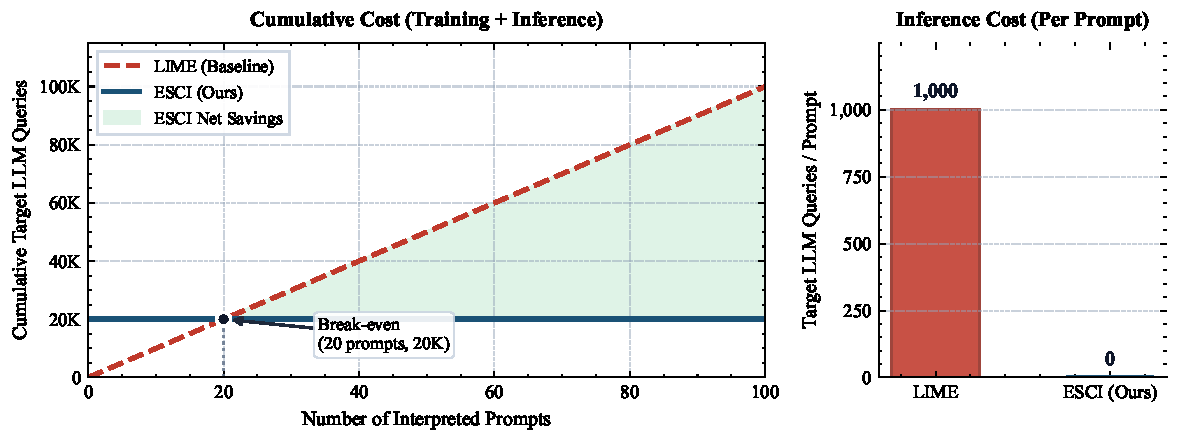
\includegraphics[width=\linewidth]{figures/Fig-INTERP-Computational-Scalability-V3.pdf}
    \caption{تحلیل مقیاس‌پذیری محاسباتی و هزینه‌ی استعلام}\label{fig:chap5_api_cost}
\end{figure}
\vspace{-0.25cm}

\paragraph{سرشکن‌سازی هزینه‌ها در \lr{ESCI}.}
در تقابل با روش‌های اختلالی، چارچوب \lr{ESCI} بخش عمده‌ی بار پردازشی را به فاز پیش‌آموزش شبکه‌ی جانشین منتقل می‌کند. پس از اتمام آموزش، استخراج انتساب برای هر ورودی جدید، نیازی به استعلام اضافی از مدل هدف نداشته و تنها با یک عبور پیش‌رو از شبکه‌ی مفسر در زمان پردازشی ثابت $\mathcal{O}(1)$ انجام می‌گیرد.

آموزش اولیه‌ی شبکه‌های انرژی و مفسر مستلزم هزینه‌ی اولیه‌ی استخراج داده است. با فرض اینکه تعداد نمونه‌های استعلام‌شده در فاز پیش‌آموزش برابر با $D_{\text{\lr{train}}} = 20000$ باشد، نقطه‌ی سربه‌سر محاسباتی میان \lr{ESCI} و خط‌پایه‌ی \lr{LIME} به‌صورت زیر محاسبه می‌گردد:
\begin{equation}
    N_{\text{\lr{break-even}}} = \frac{D_{\text{\lr{train}}}}{K_{\text{\lr{LIME\_Avg}}}} = \frac{20000}{1000} = 20
\end{equation}
این محاسبه نشان می‌دهد که هزینه‌ی اولیه‌ی آموزش چارچوب \lr{ESCI}، پس از ممیزی حدود ۲۰ پرامپت با طول متوسط در قیاس با \lr{LIME} مستهلک می‌گردد.

پویایی این مقیاس‌پذیری در شکل~\ref{fig:chap5_api_cost} نشان داده شده است. در نمودار میله‌ای سمت راست، تعداد استعلام‌های لازم در زمان استنتاج به ازای هر پرامپت مقایسه شده است که در \lr{ESCI} برابر با صفر است. در نمودار سمت چپ، روند هزینه‌ی تجمعی استعلام‌ها نشان می‌دهد که پس از نقطه‌ی سربه‌سر، هزینه‌ی حاشیه‌ای ممیزی در \lr{ESCI} ثابت می‌ماند.

\paragraph{محدودیت‌های ظرفیتی و چشم‌انداز آینده.}
در کنار مزیت محاسباتی، باید به محدودیت ظرفیت پارامتری مدل فعلی \lr{ESCI} نیز اشاره کرد. همان‌طور که در بخش‌های پیشین مشاهده شد، مفسر ۷۱ میلیون پارامتری ما در متون شدیداً ساختاریافته (نظیر \lr{WikiBio}) در تفکیک‌های ریزدانه‌ی کلید-مقدار عملکرد محتاطانه‌تری نسبت به اوراکل‌های چند میلیارد پارامتری نشان می‌دهد. فشرده‌سازی بازنمایی‌های پیچیده‌ی یک مدل زبانی بزرگ در یک جانشین نسبتاً سبک، با گلوگاه ظرفیتی همراه است. با این حال، نتایج تجربی این پژوهش اثبات می‌کند که با ارتقای مقیاس معماری مفسر و استفاده از داده‌های متنوع‌تر در آینده، می‌توان بدون از دست دادن مزیت استنتاج $\mathcal{O}(1)$، وضوح استخراج‌ها را بیش از پیش بهبود بخشید.
